% Options for packages loaded elsewhere
\PassOptionsToPackage{unicode}{hyperref}
\PassOptionsToPackage{hyphens}{url}
%
\documentclass[
]{book}
\usepackage{amsmath,amssymb}
\usepackage{lmodern}
\usepackage{ifxetex,ifluatex}
\ifnum 0\ifxetex 1\fi\ifluatex 1\fi=0 % if pdftex
  \usepackage[T1]{fontenc}
  \usepackage[utf8]{inputenc}
  \usepackage{textcomp} % provide euro and other symbols
\else % if luatex or xetex
  \usepackage{unicode-math}
  \defaultfontfeatures{Scale=MatchLowercase}
  \defaultfontfeatures[\rmfamily]{Ligatures=TeX,Scale=1}
\fi
% Use upquote if available, for straight quotes in verbatim environments
\IfFileExists{upquote.sty}{\usepackage{upquote}}{}
\IfFileExists{microtype.sty}{% use microtype if available
  \usepackage[]{microtype}
  \UseMicrotypeSet[protrusion]{basicmath} % disable protrusion for tt fonts
}{}
\makeatletter
\@ifundefined{KOMAClassName}{% if non-KOMA class
  \IfFileExists{parskip.sty}{%
    \usepackage{parskip}
  }{% else
    \setlength{\parindent}{0pt}
    \setlength{\parskip}{6pt plus 2pt minus 1pt}}
}{% if KOMA class
  \KOMAoptions{parskip=half}}
\makeatother
\usepackage{xcolor}
\IfFileExists{xurl.sty}{\usepackage{xurl}}{} % add URL line breaks if available
\IfFileExists{bookmark.sty}{\usepackage{bookmark}}{\usepackage{hyperref}}
\hypersetup{
  pdftitle={Versuchsplanung},
  pdfauthor={Max Brede und Maren Hinck},
  hidelinks,
  pdfcreator={LaTeX via pandoc}}
\urlstyle{same} % disable monospaced font for URLs
\usepackage{longtable,booktabs,array}
\usepackage{calc} % for calculating minipage widths
% Correct order of tables after \paragraph or \subparagraph
\usepackage{etoolbox}
\makeatletter
\patchcmd\longtable{\par}{\if@noskipsec\mbox{}\fi\par}{}{}
\makeatother
% Allow footnotes in longtable head/foot
\IfFileExists{footnotehyper.sty}{\usepackage{footnotehyper}}{\usepackage{footnote}}
\makesavenoteenv{longtable}
\usepackage{graphicx}
\makeatletter
\def\maxwidth{\ifdim\Gin@nat@width>\linewidth\linewidth\else\Gin@nat@width\fi}
\def\maxheight{\ifdim\Gin@nat@height>\textheight\textheight\else\Gin@nat@height\fi}
\makeatother
% Scale images if necessary, so that they will not overflow the page
% margins by default, and it is still possible to overwrite the defaults
% using explicit options in \includegraphics[width, height, ...]{}
\setkeys{Gin}{width=\maxwidth,height=\maxheight,keepaspectratio}
% Set default figure placement to htbp
\makeatletter
\def\fps@figure{htbp}
\makeatother
\setlength{\emergencystretch}{3em} % prevent overfull lines
\providecommand{\tightlist}{%
  \setlength{\itemsep}{0pt}\setlength{\parskip}{0pt}}
\setcounter{secnumdepth}{5}
\usepackage{booktabs}
\usepackage{tikz}

\newenvironment{cols}[1][]{}{}

\newenvironment{col}[1]{\begin{minipage}{#1}\ignorespaces}{%
\end{minipage}
\ifhmode\unskip\fi
\aftergroup\useignorespacesandallpars}

\def\useignorespacesandallpars#1\ignorespaces\fi{%
#1\fi\ignorespacesandallpars}

\makeatletter
\def\ignorespacesandallpars{%
  \@ifnextchar\par
    {\expandafter\ignorespacesandallpars\@gobble}%
    {}%
}
\makeatother

\usetikzlibrary{arrows, arrows.meta, calc, positioning, quotes, shapes}
\tikzset{
    mynode/.style={draw,text width=1in,align=center},
    mylabel/.style={text width=7em}
}

\definecolor{White}{gray}{1}
\definecolor{Black}{gray}{0}
\definecolor{Gray}{gray}{0.5}
\definecolor{LightGray}{gray}{0.99}
\definecolor{DarkGray}{gray}{0.6}
\definecolor{LightBlue}{rgb}{0.9 0.9 1}
\definecolor{Blue}{rgb}{0.55 0.55 1}
\definecolor{DarkBlue}{rgb}{0.2 0.2 1}
\definecolor{Red}{rgb}{1 0 0}
\definecolor{DarkRed}{rgb}{0.7 0 0}
\definecolor{Green}{rgb}{0 0.8 0.2}


\usepackage{lscape}
\newcommand{\blandscape}{\begin{landscape}}
\newcommand{\elandscape}{\end{landscape}}
\usepackage{booktabs}
\usepackage{longtable}
\usepackage{array}
\usepackage{multirow}
\usepackage{wrapfig}
\usepackage{float}
\usepackage{colortbl}
\usepackage{pdflscape}
\usepackage{tabu}
\usepackage{threeparttable}
\usepackage{threeparttablex}
\usepackage[normalem]{ulem}
\usepackage{makecell}
\usepackage{xcolor}
\usepackage{caption}
\usepackage{graphicx}
\usepackage{siunitx}
\usepackage{ulem}
\usepackage{hhline}
\usepackage{calc}
\usepackage{tabularx}
\usepackage{adjustbox}
\usepackage{hyperref}
\ifluatex
  \usepackage{selnolig}  % disable illegal ligatures
\fi
\usepackage[]{natbib}
\bibliographystyle{apalike}

\title{Versuchsplanung}
\author{Max Brede und Maren Hinck}
\date{2021-01-24}

\begin{document}
\maketitle

{
\setcounter{tocdepth}{1}
\tableofcontents
}
\hypertarget{vorwort}{%
\chapter{Vorwort}\label{vorwort}}

Dieses mit \texttt{bookdown} erstellte Dokument ist das über das Wintersemester 2020 hinweg wachsende Skript zum Seminar ``PSY\_B\_4: Versuchsplanung'' der CAU zu Kiel.

\hypertarget{lehrplan}{%
\chapter{Lehrplan}\label{lehrplan}}

\hypertarget{semesterplan}{%
\section{Semesterplan}\label{semesterplan}}

\blandscape
\scriptsize

\begin{longtable}[t]{>{\raggedright\arraybackslash}p{0.33in}>{\raggedright\arraybackslash}p{0.4in}>{\raggedright\arraybackslash}p{0.7in}>{\raggedright\arraybackslash}p{1.5in}>{\raggedright\arraybackslash}p{2.5in}>{\raggedright\arraybackslash}p{0.75in}}
\toprule
Sitzung & Datum & Sitzungstitel & Unterkapitel & Lernziele & Hausaufgaben\\
\midrule
 &  &  &  & Die Studierenden… & \\
1 & 02.11.2020 & Warum wissenschaftliche Psychologie & Alltagspsychologie und ihre Fehler & … können typische Urteilsfehler, Wahrnehmungsverzerrungen und Erwartungseffekte erkennen und beschreiben & Kapitel 1, 2\\
 &  &  & Theorien und wissenschaftliches Vorgehen & … können die Beziehung zwischen Theorie, Hypothese und Variable erklären & Fragestellungen einsenden\\
2 & 28.11.2020
29.11.2020 & Hypothesen und der Prozess der Hypothesenprüfung & Vorgehen beim Hypothesentesten & … können die wesentlichen Schritte beim Testen einer psychologischen Hypothese aufzählen und beschreiben, was in jedem Schritt anfällt & Kapitel 3\\
 &  &  & Hypothesen & … können eine Reihe von Gütekriterien von Hypothesen nennen & \\
\addlinespace
3 & 28.11.2020
29.11.2020 & Experimentelles Vorgehen & Experiment und Kausalschlüsse & … können verschiedene Probleme, die beim nicht-experimentellen Vorgehen Kausalschlüsse verhindern können, aufzählen & Kapitel 4.1\\
 &  &  &  & … können die Definitionsmerkmale eines Experiments aufzählen und anhand dieser experimenteller von nicht-experimenteller Forschung unterscheiden & \\
 &  &  & Variablen im Experiment & … können die Begriffe UV, AV, Störvariable, VL, VP definieren & \\
 &  &  & Nicht-experimentelle Studientypen & … können die Unterschiede zwischen Experimenten, Quasi-Experimenten, Ex-Post-Facto-Studien und Nichtexperimentellen Studien nennen und entsprechende Studien kategorisieren & \\
4 & 28.11.2020
29.11.2020 & Literaturrecherche & Literaturrecherche & … können verschiedene Anlaufstellen zur Akquise von Literatur aufzählen und haben erste Erfahrungen in deren Nutzung & Kapitel 4.2\\
\addlinespace
 &  &  &  & … kennen Ansätze zum Vorgehen bei der Literaturrecherche und können diese anwenden & Abstract und Introduction von jeweils einer der gefundenen Studien lesen\\
5 & 28.11.2020
29.11.2020 & Operationalisieren und Messen & Operationalisierung & … können den Begriff Operationalisierung definieren & Kapitel 4.3, 5\\
 &  &  &  & … können anhand einer Reihe von Beschreibungsmaßen die Güte einer Operationalisierung einschätzen & \\
 &  &  & Das Messen und dessen Probleme & … können die ‚Problemkreise beim Messen‘ nennen & \\
 &  &  & Beispiele für Messmethoden & … können typische Beispiele für psychologische Messmethoden aufzählen und grob erläutern & \\
\addlinespace
 &  &  &  & … können anhand einer Hypothese und der nötigen Konstruktes eine geeignete Operationalisierung entwerfen & \\
6 & 12.12.2020
13.12.2020 & Experimentelle Versuchspläne & Einfaktorielle Versuchspläne & … können verschiedene einfaktorielle experimentelle Designs erkennen und diese tabellarisch darstellen & Kapitel 6,7\\
 &  &  &  & … können den Unterschied zwischen within- und between-Faktoren erklären & \\
 &  &  & Mehrfaktoriele Versuchspläne & … können verschiedene mehrfaktorielle experimentelle Designs erkennen und diese tabellarisch darstellen & \\
7 & 12.12.2020
13.12.2020 & Störvariablen im Experiment & Messfehler vs. Störvariable & … können erklären, was Konfundierung bedeutet und kennen das Konzept der Varianzzerlegung in Primär-, Sekundärvarianz und Zufallsfehler & Kapitel 8\\
\addlinespace
 &  &  & Störvariablen in der Person & … können Carry-Over-Effekte und Positionseffekte  und  den Umgang mit diesen erklären & \\
 &  &  & Störvariablen in der Untersuchungssituation & … können VL-Erwartungseffekte, VP-Erwartungseffekte und motivationale Faktoren auf Seite der VP als Störvariablen  und  den Umgang mit diesen erklären & \\
8 & 12.12.2020
13.12.2020 & Nicht-experimentelle Versuchspläne & Quasi-Experimente & … können verschiedene Quasi-experimentelle Designs erkennen und  deren Vor- und Nachteile aufzählen & Kapitel 4.4, 4.5, 4.7\\
 &  &  & Andere Studientypen & … können verschiedene nicht-experimentelle Designs erkennen und  deren Vor- und Nachteile aufzählen & \\
9 & 12.12.2020
13.12.2020 & Material und Stichprobe & Stichprobe & … können verschiedene Strategien zur Stichprobenziehung und Zusammensetzung und deren jeweilige Vor- und Nachteile beschreiben & Kapitel 4.6, 4.8\\
\addlinespace
10 & 23.1.2021
24.1.2021 & Auswertung, Darstellung und Interpretation & Arten statistischer Hypothesen & … können die Namen grundlegender statistischer Verfahren erkennen und jeweils Beispiele nennen, für welche Art von Fragestellung der jeweilige Test anzuwenden ist. & Kapitel 9\\
 &  &  &  & … können Unterschieds- und Zusammenhangshypothesen formal korrekt formulieren & \\
 &  &  &  & … können Scatter-, Bar-  und Boxplots erkennen und aus ihnen deskriptive Aussagen ableiten & \\
 &  &  & Vermeidbare Fehler & … erkennen einige häufige Fehler in der Erstellung von den o.g. Darstellungsformen und Hypothesen und können diese vermeiden & \\
11 & 23.1.2021
24.1.2021 & Ethische Probleme im Versuch & Ethische Probleme & … können die wichtigsten Arten von ethischen Problemen in psychologischen Experimenten aufzählen und können jeweils erklären, wie man diese entschärfen kann & Kapitel 4.9\\
\addlinespace
12 & 23.1.2021
24.1.2021 & Publikationsprozess & Aufbau einer Publikation & … können in einem psychologischen paper den Abschnitt nennen, in dem eine gesuchte Information wahrscheinlich zu finden ist & Präsentation für Termin 13 vorbereiten\\
 &  &  & Publikationsprozess & … können den Begriff des Peer-Reviews erklären und wissen was ein Journal-Impact-Faktor ist & \\
 &  &  & wissenschaftliches Fehlverhalten & … können häufige Fälle wissenschaftlichen Fehlverhaltens nennen und vermeiden & \\
13 & wird noch bekannt gegeben & Vorstellung der Gruppenarbeiten &  & … haben grundlegende Erfahrungen im Aufbereiten und Präsentieren eigener Forschungsarbeiten & \\
14 & wird noch bekannt gegeben & Klausurvorbereitung &  & … haben keine Angst mehr vor der Klausur & \\
\bottomrule
\end{longtable}
\normalsize
\elandscape
\newpage

\hypertarget{warum-wissenschaftliche-psychologie}{%
\chapter{Warum wissenschaftliche Psychologie?}\label{warum-wissenschaftliche-psychologie}}

\hypertarget{organisatorisches}{%
\section{Organisatorisches}\label{organisatorisches}}

\hypertarget{pruxfcfungsleistung}{%
\subsection*{Prüfungsleistung}\label{pruxfcfungsleistung}}
\addcontentsline{toc}{subsection}{Prüfungsleistung}

\begin{itemize}
\tightlist
\item
  Klausur

  \begin{itemize}
  \tightlist
  \item
    3-tägige Take-Home-Klausur
  \item
    Ausgabe am 22.2.21
  \end{itemize}
\item
  Prüfungsvorleistung

  \begin{itemize}
  \tightlist
  \item
    Erstellung eines eigenen Versuchsplans, Darstellung in Form einer Hausarbeit
  \item
    Leseaufgaben und Bearbeitung der jeweiligen Fragen zum Kapitel im Olat
  \end{itemize}
\end{itemize}

\hypertarget{literatur}{%
\subsection*{Literatur}\label{literatur}}
\addcontentsline{toc}{subsection}{Literatur}

\citet{huberPsychologischeExperiment2019} Das psychologische Experiment. Eine Einführung. Bern: Hans Huber.

\hypertarget{semesterplan-1}{%
\subsection{Semesterplan}\label{semesterplan-1}}

\small

\begin{tabular}[t]{rll}
\toprule
Sitzung & Datum & Sitzungstitel\\
\midrule
1 & 02.11.2020 & Warum wissenschaftliche Psychologie\\
2 & 28.11.2020
29.11.2020 & Hypothesen und der Prozess der Hypothesenprüfung\\
3 & 28.11.2020
29.11.2020 & Experimentelles Vorgehen\\
4 & 28.11.2020
29.11.2020 & Literaturrecherche\\
5 & 28.11.2020
29.11.2020 & Operationalisieren und Messen\\
\addlinespace
6 & 12.12.2020
13.12.2020 & Experimentelle Versuchspläne\\
7 & 12.12.2020
13.12.2020 & Störvariablen im Experiment\\
8 & 12.12.2020
13.12.2020 & Nicht-experimentelle Versuchspläne\\
9 & 12.12.2020
13.12.2020 & Material und Stichprobe\\
10 & 23.1.2021
24.1.2021 & Auswertung, Darstellung und Interpretation\\
\addlinespace
11 & 23.1.2021
24.1.2021 & Ethische Probleme im Versuch\\
12 & 23.1.2021
24.1.2021 & Publikationsprozess\\
13 & wird noch bekannt gegeben & Vorstellung der Gruppenarbeiten\\
14 & wird noch bekannt gegeben & Klausurvorbereitung\\
\bottomrule
\end{tabular}

\hypertarget{alltagspsychologie-und-ihre-fehler}{%
\section{Alltagspsychologie und ihre Fehler}\label{alltagspsychologie-und-ihre-fehler}}

\hypertarget{was-ist-psychologie}{%
\subsection{Was ist Psychologie?}\label{was-ist-psychologie}}

Was meinen Sie?
Was ist die Aufgabe der Psychologie?

\hypertarget{was-ist-mit-alltagspsychologie-gemeint}{%
\subsection{Was ist mit Alltagspsychologie gemeint?}\label{was-ist-mit-alltagspsychologie-gemeint}}

\begin{itemize}
\tightlist
\item
  Männer haben weniger Empathie als Frauen.\smallskip
\item
  Liebe wächst mit der Entfernung vs.~Aus den Augen, aus dem Sinn \smallskip
\item
  Alle Psychologie-Studierenden studieren nur, um sich selbst zu therapieren. \smallskip
\item
  Alle mexikanischen Einwanderer sind kriminell
\end{itemize}

\hypertarget{woher-kommen-solche-aussagen}{%
\subsection{Woher kommen solche Aussagen?}\label{woher-kommen-solche-aussagen}}

\begin{itemize}
\tightlist
\item
  `Bauchgefühl' \smallskip
\item
  `Erfahrungswerte' \smallskip
\item
  `gesundem Menschenverstand'
\end{itemize}

Oft sind diese Arten intuitiven Vorgehens vernünftig, weil sie ständiges Hinterfragen von Denken und Handeln verhindern, und häufig zu richtigen Entscheidungen führen. (Stichwort ökologische Rationalität)\medskip

Um zu verstehen, warum diese intuitiven Vorgehensweisen kein guter Standard für den Erkenntnisgewinn sind, wollen wir auf ein paar Stolpersteine in der Wahrnehmung, Beurteilung und dem Abrufen von Informationen eingehen, die unter Umständen zu Fehlurteilen führen können

\hypertarget{wahrnehmung-von-informationen}{%
\subsection{Wahrnehmung von Informationen}\label{wahrnehmung-von-informationen}}

\hypertarget{muxfcller-lyer-effekt}{%
\subsubsection{Müller-Lyer-Effekt}\label{muxfcller-lyer-effekt}}

\begin{center}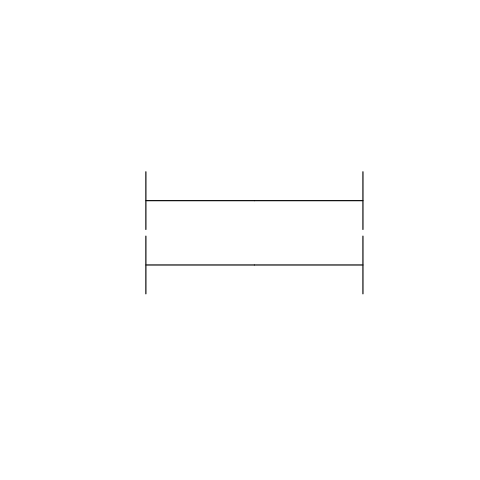
\includegraphics[width=6.67in,height=0.25\textheight]{imgs/some} \end{center}

\begin{center}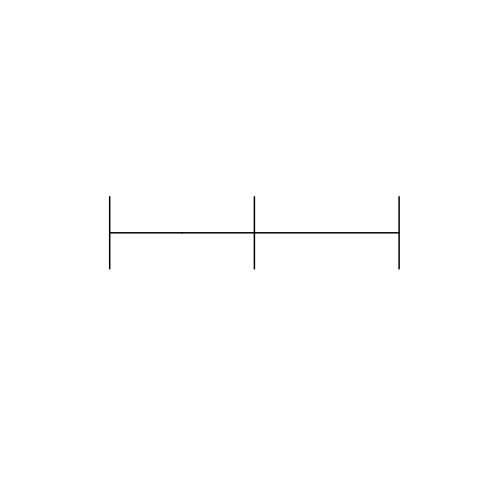
\includegraphics[width=6.67in,height=0.25\textheight]{imgs/some2} \end{center}

\begin{center}\rule{0.5\linewidth}{0.5pt}\end{center}

\hypertarget{selektive-aufmerksamkeit}{%
\subsubsection{selektive Aufmerksamkeit}\label{selektive-aufmerksamkeit}}

Unter welchem Hütchen ist die Praline?

\textbf{typische Wahrnehmungs-`Fehler':}

\begin{itemize}
\item
  `Fehlwahrnehmungen'
\item
  selektive Aufmerksamkeit
\item
  \textbf{Halo-Effekt:} Tendenz faktisch unabhängige oder nur mäßig korrelierende Eigenschaften von Personen oder Sachen
  fälschlicherweise als zusammenhängend wahrzunehmen.

  \begin{itemize}
  \tightlist
  \item
    z.B. die bessere schriftliche Benotung von Schülern ohne inhaltlichen Grund, wenn sie mit hoher Quantität mündliche Beteiligung gezeigt haben
  \end{itemize}
\item
  \textbf{Bestätigungsfehler:} Tendenz Informationen so auszuwählen, zu ermitteln und zu interpretieren, dass diese die
  eigenen Erwartungen erfüllen.

  \begin{itemize}
  \tightlist
  \item
    z.B. das Gefühl, wahrnehmen zu können, wenn man beobachtet wird
  \end{itemize}
\item
  \textbf{Erwartungseffekte} Die Beeinflussung des Ergebnisses einer Situation durch die Erwartungen an diese. Dazu später mehr.
\end{itemize}

\hypertarget{beurteilung-von-informationen}{%
\subsection{Beurteilung von Informationen}\label{beurteilung-von-informationen}}

\hypertarget{umfrage-auf-limesurvey}{%
\subsubsection{Umfrage auf LimeSurvey:}\label{umfrage-auf-limesurvey}}

\begin{figure}

{\centering 
\includegraphics[width=250pt]{imgs/AnkerAutoritaet} 

}

\caption{Schätzfragen [https://tinyurl.com/y7yyjltd](https://tinyurl.com/y7yyjltd)}\label{fig:unnamed-chunk-8}
\end{figure}

\hypertarget{schuxe4tzfrage}{%
\subsubsection{Schätzfrage}\label{schuxe4tzfrage}}

Wie lang ist der Nord-Ostsee-Kanal, was schätzen Sie? Der Nord-Ostsee-Kanal geht von Kiel an der Ostsee bis Brunsbüttel an der Nordsee. Der \textbf{1. Vorstand des Bayerischen Dachshundklubs, Herr Jürgen Bujanowski-Weber} / \textbf{frühere Ministerpräsident des Landes Schleswig-Holstein, Herr Peter Harry Carstensen} , schätzte die Länge des Nord-Ostsee-Kanals auf \textbf{50} / \textbf{200} km. \medskip

Wie viele Länder liegen auf dem afrikanischen Kontinent, was schätzen Sie? Afrika ist einer der Kontinente der Erde. Seine Fläche von 30,2 Millionen km² entspricht etwa 22 \% der gesamten Landfläche des Planeten, er hatte 2017 eine Bevölkerung von circa 1,3 Milliarden Menschen. Der \textbf{ehemalige Präsident der Republik Südafrika, Nelson Mandela} / \textbf{Präsident der Vereinigten Staaten von Amerika, Donald Trump}, schätzte die Anzahl der afrikanischen Länder auf \textbf{25} / \textbf{85}.

\hypertarget{urteilsheuristiken}{%
\subsubsection{Urteilsheuristiken}\label{urteilsheuristiken}}

Auswertung \href{hier}{https://mbrede.shinyapps.io/VPlanung/}

\hypertarget{anagramme}{%
\subsubsection{Anagramme}\label{anagramme}}

\begin{longtable}[]{@{}lll@{}}
\toprule
\endhead
SERWAS & \(\rightarrow\) & WASSER \\ \addlinespace
TESSMY & \(\rightarrow\) & SYSTEM \\ \addlinespace
HARTOX & \(\rightarrow\) & THORAX \\ \addlinespace
\bottomrule
\end{longtable}

\hypertarget{anagramme-1}{%
\subsubsection{Anagramme}\label{anagramme-1}}

\hypertarget{um-das-zu-luxf6sen-bruxe4uchte-ich}{%
\paragraph{Um das zu lösen bräuchte ich:}\label{um-das-zu-luxf6sen-bruxe4uchte-ich}}

\begin{enumerate}
\def\labelenumi{\Alph{enumi})}
\tightlist
\item
  0-15 Sek
\item
  16-30 Sek.
\item
  31-45 Sek.
\item
  46-60 Sek.
\item
  mehr als eine Minute
\end{enumerate}

\hypertarget{anagramme-2}{%
\subsubsection{Anagramme}\label{anagramme-2}}

\begin{longtable}[]{@{}lll@{}}
\toprule
\endhead
CAHENFI & \(\rightarrow\) & ??? \\ \addlinespace
\bottomrule
\end{longtable}

\hypertarget{exkurs-korrelation}{%
\subsubsection{Exkurs: Korrelation}\label{exkurs-korrelation}}

Der Begriff Korrelation beschreibt einen Zusammenhang zweier oder mehrerer Merkmale.

In der Psychologie ist meistens die \emph{`Pearson-Korrelation'} gemeint. Diese stellt ein Maß für den \emph{linearen} Zusammenhang zweier Variablen dar.

\hypertarget{pearson-korrelation}{%
\subsubsection{Pearson-Korrelation:}\label{pearson-korrelation}}

\medskip

\begin{tabular}{c| c| c| c| c| c| c| c| c| c| c}
 x&5&2&3&1&1&5&2&7&9&5 \\ \hline 
 y&9&4&7&2&5&6&5&6&9&6 \\ 
\end{tabular}
\medskip

\begin{center}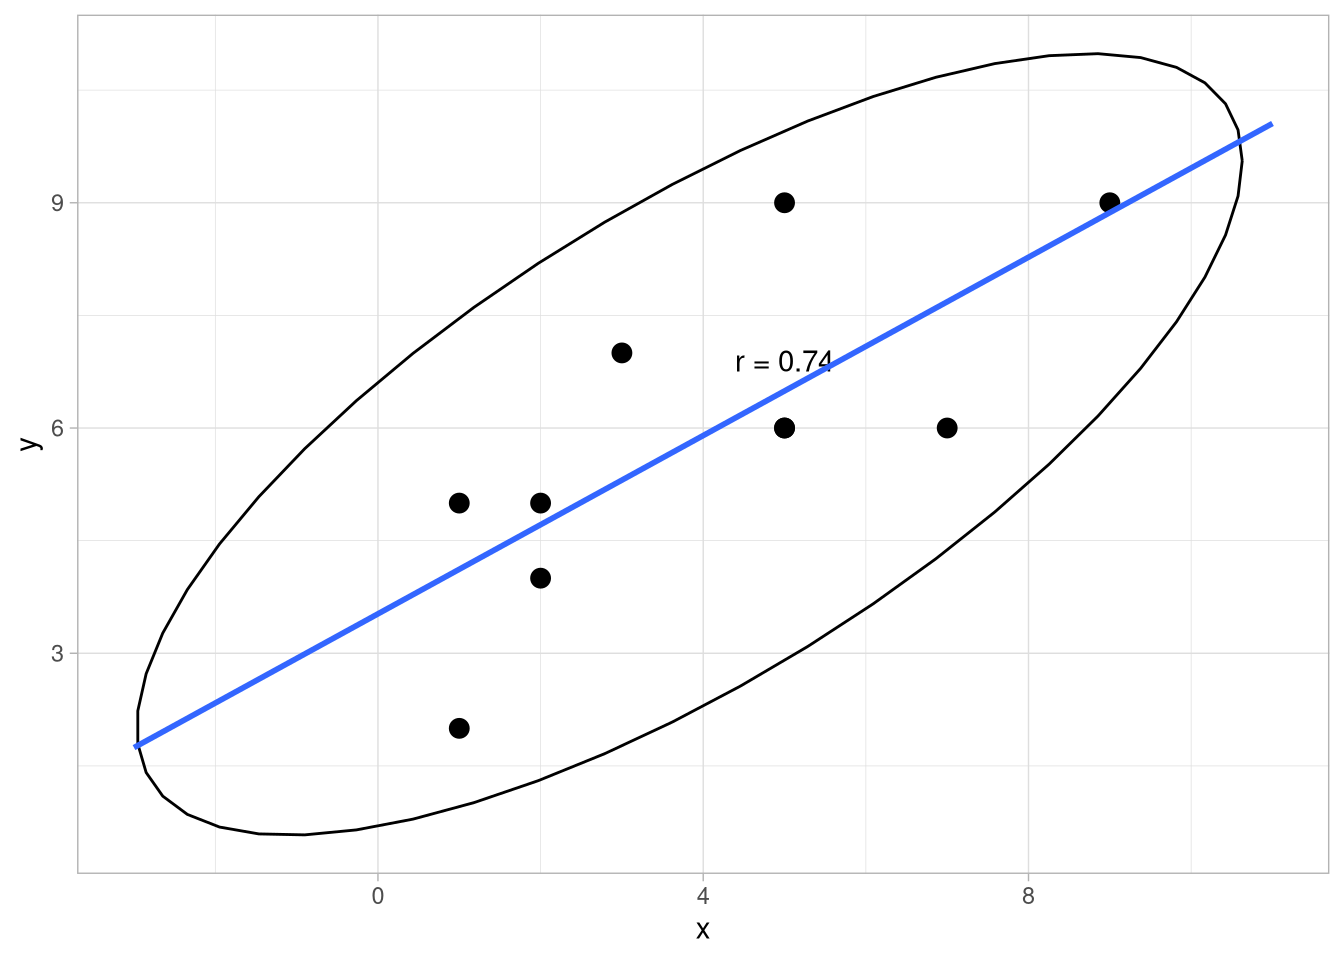
\includegraphics{Versuchsplanung_WS20_files/figure-latex/unnamed-chunk-11-1} \end{center}

\medskip

\begin{center}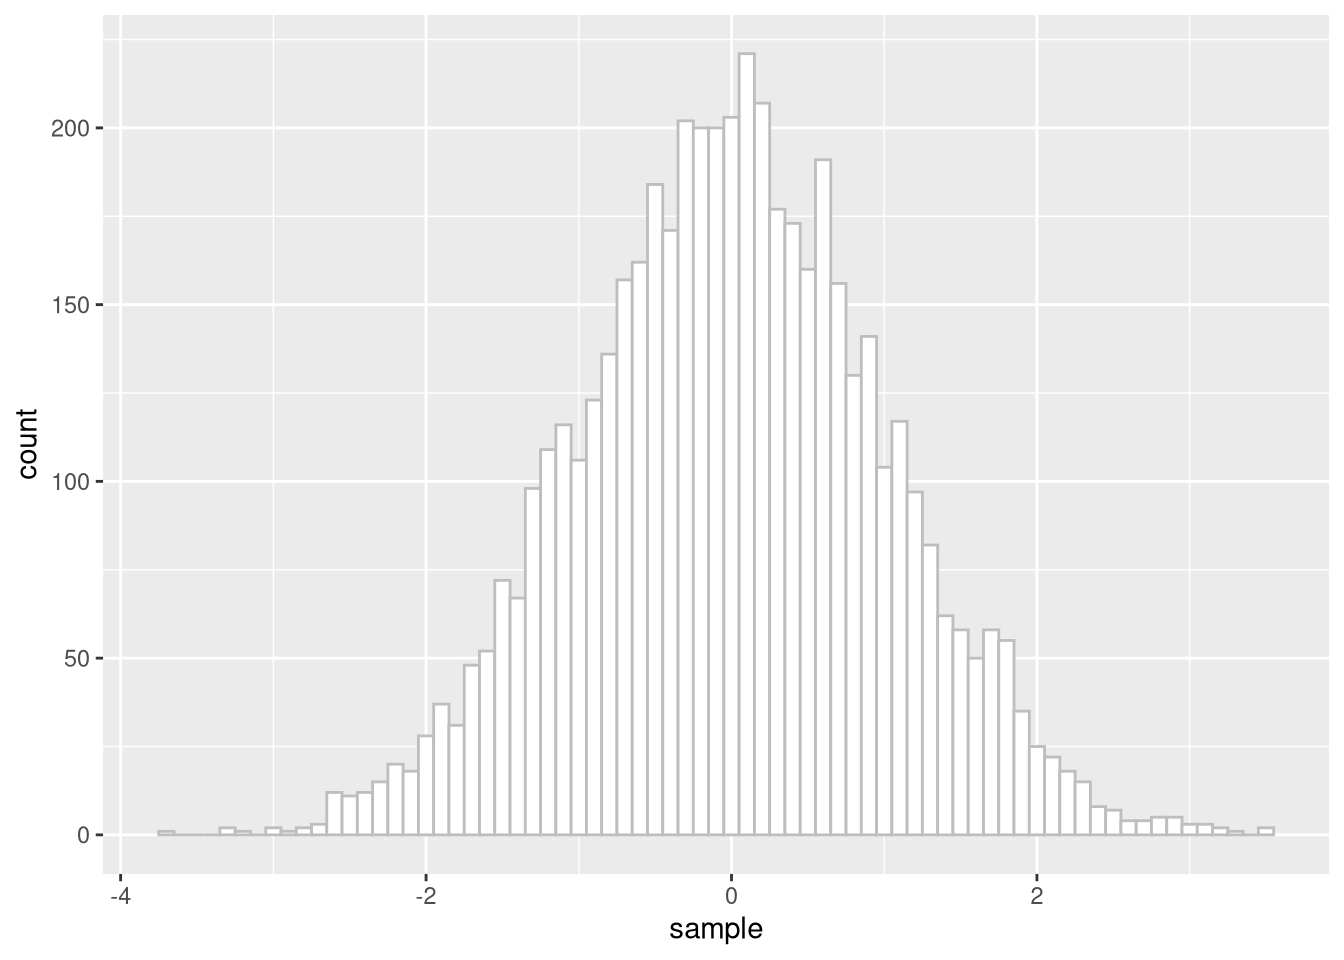
\includegraphics{Versuchsplanung_WS20_files/figure-latex/unnamed-chunk-12-1} \end{center}

Dabei gibt es zwei Fallstricke:

\begin{enumerate}
\def\labelenumi{\arabic{enumi}.}
\item
  Pearson-Korrelationen geben nur Aussage über \emph{lineare} Zusammenhänge
\item
  Eine Korrelation zu finden, bedeutet nicht gleich einen Kausalzusammenhang gefunden zu haben
\end{enumerate}

\hypertarget{linearzusammenhuxe4nge}{%
\subsubsection{Linearzusammenhänge}\label{linearzusammenhuxe4nge}}

\begin{center}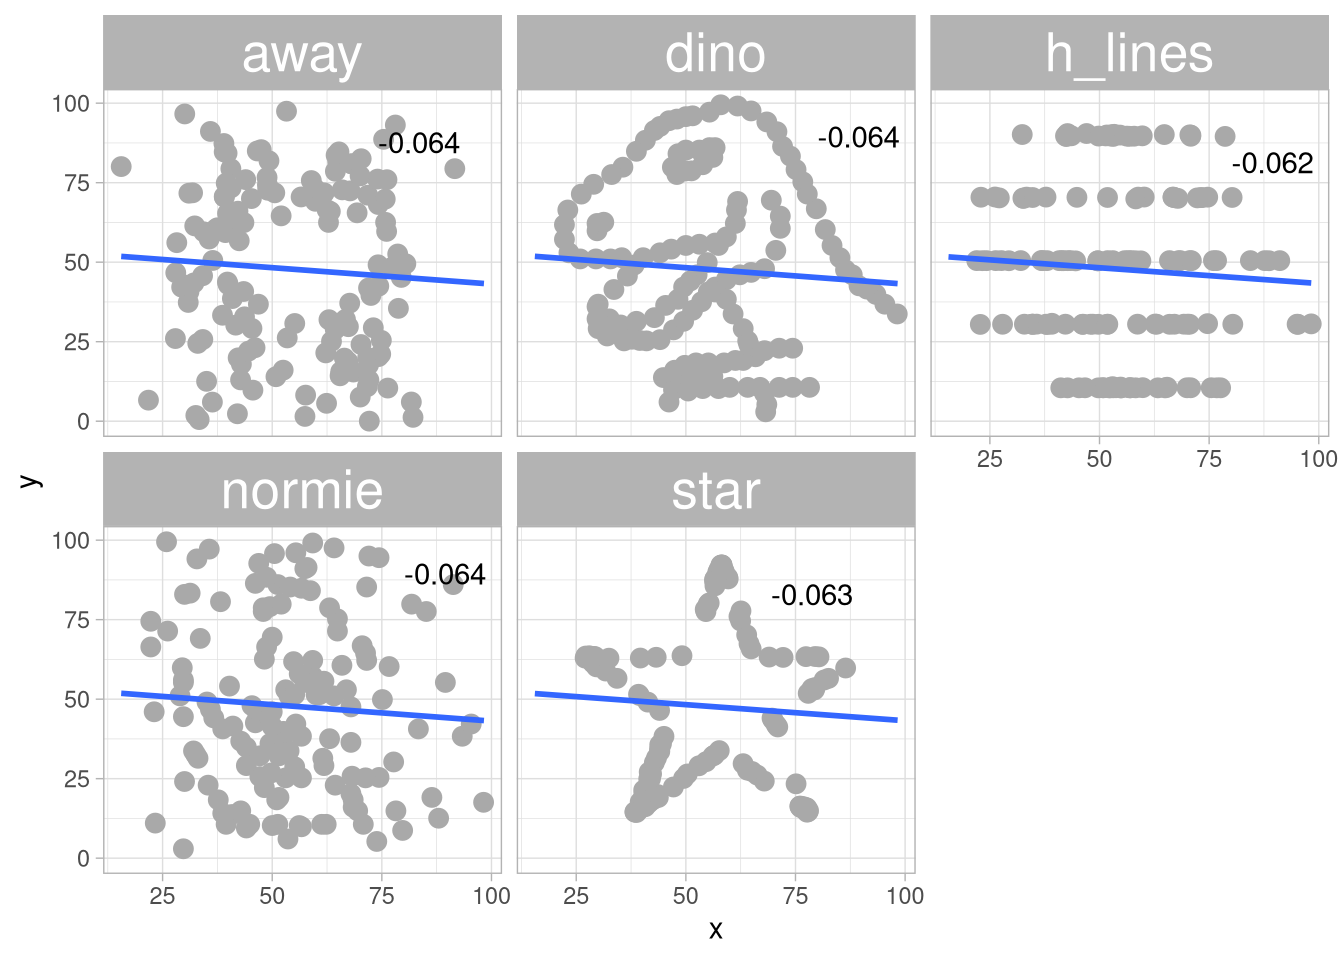
\includegraphics{Versuchsplanung_WS20_files/figure-latex/unnamed-chunk-13-1} \end{center}

\hypertarget{korrelation-vs.-kausalituxe4t}{%
\subsection{Korrelation vs.~Kausalität}\label{korrelation-vs.-kausalituxe4t}}

Aber selbst wenn ein linearer Zusammenhang besteht, bedeutet der nicht unbedingt einen kausalen Zusammenhang:

\begin{tabular}[t]{lrrrr}
\toprule
Country & Area & Storks & Humans.mio. & BirthRate.kPerYear.\\
\midrule
Albania & 28750 & 100 & 3.2 & 83\\
Austria & 83860 & 300 & 7.6 & 87\\
Belgium & 30520 & 1 & 9.9 & 118\\
Bulgaria & 111000 & 5000 & 9.0 & 117\\
Denmark & 43100 & 9 & 5.1 & 59\\
\addlinespace
France & 544000 & 140 & 56.0 & 774\\
Germany & 357000 & 3300 & 78.0 & 901\\
Greece & 132000 & 2500 & 10.0 & 106\\
Holland & 41900 & 4 & 15.0 & 188\\
Hungary & 93000 & 5000 & 11.0 & 124\\
\addlinespace
Italy & 301280 & 5 & 57.0 & 551\\
Poland & 312680 & 30000 & 38.0 & 610\\
Portugal & 92390 & 1500 & 10.0 & 120\\
Romania & 237500 & 5000 & 23.0 & 367\\
Spain & 504750 & 8000 & 39.0 & 439\\
\addlinespace
Switzerland & 41290 & 150 & 6.7 & 82\\
Turkey & 779450 & 25000 & 56.0 & 1576\\
\bottomrule
\end{tabular}

Tabelle aus: Matthews, R. (2000). Storks deliver babies (p= 0.008). \emph{Teaching Statistics, 22}(2), 36-38.

\begin{center}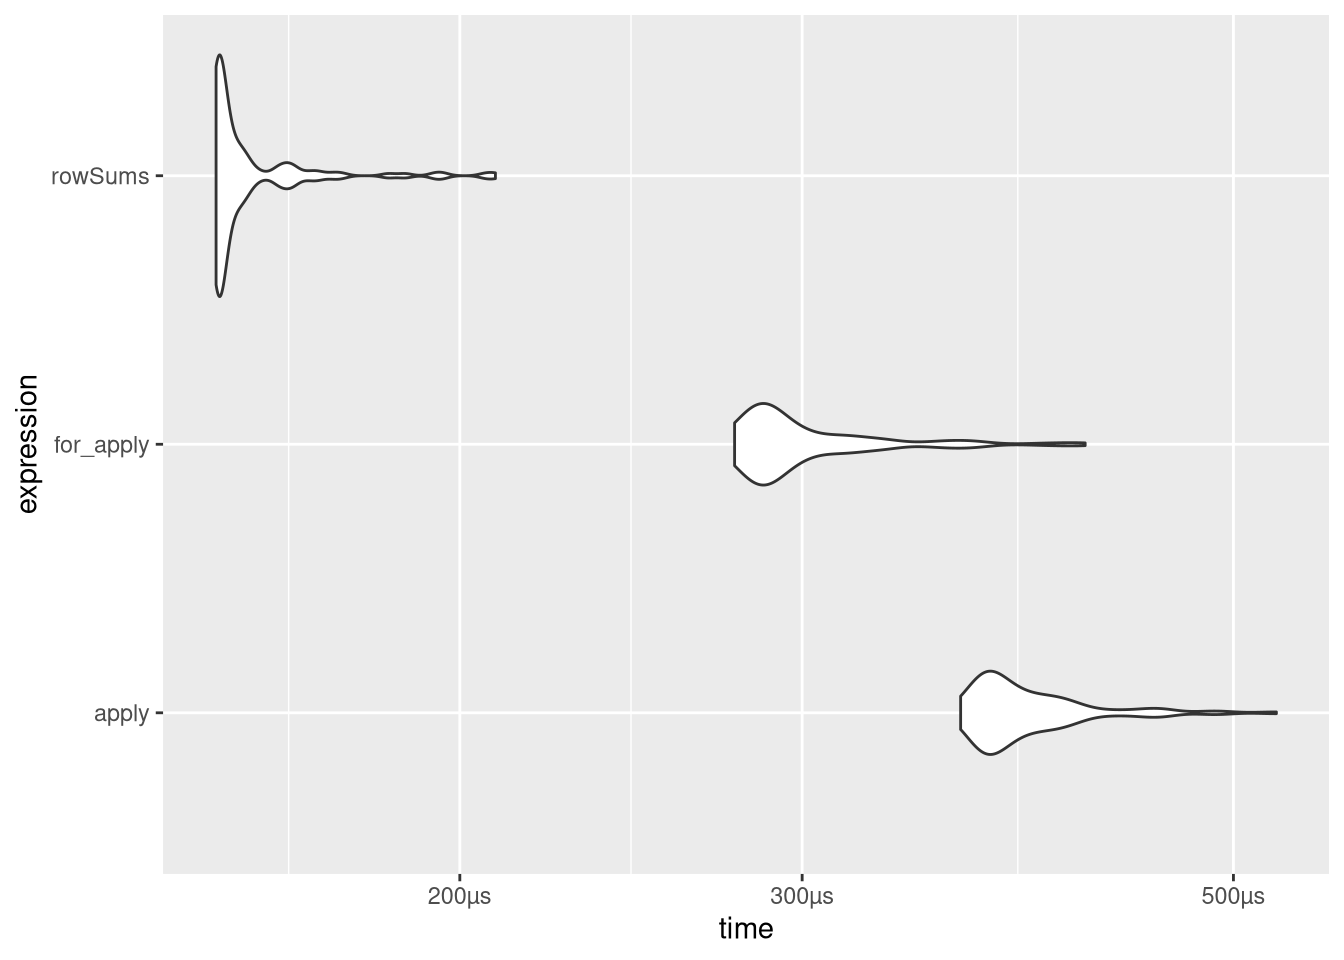
\includegraphics{Versuchsplanung_WS20_files/figure-latex/unnamed-chunk-15-1} \end{center}

\hypertarget{typische-beurteilungs-fehler}{%
\subsubsection{typische Beurteilungs-`Fehler'}\label{typische-beurteilungs-fehler}}

\begin{itemize}
\item
  Ankerheuristik
\item
  Orientierung an Autoritäten
\item
  overconfidence/Selbstüberschätzung
\item
  Korrelation vs.~Kausalität
\item
  \textbf{Rekognitionsheuristik:} Die Tendenz dazu, dazu zu neigen, bei einer Entscheidung zwischen zwei Alternativen diejenige als höher/größer/besser zu bewerten die einem bekannt vorkommt

  \begin{itemize}
  \tightlist
  \item
    z.B.: San Diego vs.~San Antonio
  \end{itemize}
\end{itemize}

\hypertarget{abruf-von-informationen}{%
\subsection{Abruf von Informationen}\label{abruf-von-informationen}}

\hypertarget{umfrage-auf-limesurvey-1}{%
\subsubsection{Umfrage auf LimeSurvey:}\label{umfrage-auf-limesurvey-1}}

\begin{figure}

{\centering 
\includegraphics[width=250pt]{imgs/Hindsight} 

}

\caption{Schätzfragen [https://tinyurl.com/y8mebw22](https://tinyurl.com/y8mebw22)}\label{fig:unnamed-chunk-16}
\end{figure}

\hypertarget{hindsightbias}{%
\subsection{Hindsightbias}\label{hindsightbias}}

Auswertung \href{hier}{https://mbrede.shinyapps.io/VPlanung/}

\hypertarget{fazit}{%
\subsection{Fazit}\label{fazit}}

Auf verschiedenen Ebenen der intuitiven Informationsverarbeitungen können Fehler auftreten, die zu einem falschen Ergebnis führen.

Wir brauchen für unsere psychologische Arbeit also eine andere Methodik.

\hypertarget{wissenschaftliche-psychologie}{%
\section{Wissenschaftliche Psychologie}\label{wissenschaftliche-psychologie}}

\hypertarget{wissenschaftliche-methodik}{%
\subsection{Wissenschaftliche Methodik}\label{wissenschaftliche-methodik}}

Wissenschaftliche Psychologie in Abgrenzung zur Alltagspsychologie zeichnet sich dadurch aus, dass sie wissenschaftliche Methodik im Gegensatz zu intuitiven Schlüssen nutzt, um zu Erkenntnissen zu gelangen.

Aber was heißt `wissenschaftliche Methodik' denn nun?

\hypertarget{wissenschaftliches-vorgehen-im-allgemeinen}{%
\subsection{Wissenschaftliches Vorgehen im Allgemeinen}\label{wissenschaftliches-vorgehen-im-allgemeinen}}

Ein paar von vielen wichtigen Begriffen in der Abgrenzung von wissenschaftlicher zu nicht-wissenschaftlicher Methodik:

\begin{itemize}
\tightlist
\item
  Theorien - Phänomene - Modelle
\item
  Fragestellung - Hypothesen - Variablen \smallskip
\item
  Falsifikationsprinzip nach Popper \smallskip
\end{itemize}

Für ein gemeinsames Verständnis vom Inhalt der Begriffe hier eine kurze Begriffserklärung:

\hypertarget{phuxe4nomen}{%
\subsubsection{Phänomen:}\label{phuxe4nomen}}

Eine wiederkehrende Beobachtung, deren genauere Untersuchung relevant erscheint.

\hypertarget{theorie}{%
\subsubsection{Theorie:}\label{theorie}}

Zusammenhängendes System von allgemeinen wissenschaftlichen Aussagen
welches einen Teilbereich der Realität (das Phänomen) beschreibt und erklärt.

\hypertarget{modell}{%
\subsubsection{Modell:}\label{modell}}

Formale Struktur, oftmals eine Analogie, welche den Kern einer Theorie
veranschaulicht und Ableitungen von Hypothesen erleichtern soll.

\hypertarget{fragestellung}{%
\subsubsection{Fragestellung:}\label{fragestellung}}

Eine interessant erscheinende, durch wissenschaftliche Methoden zu beantwortende Frage, die sich auf Implikationen der Theorie bezieht.

\hypertarget{hypothese}{%
\subsubsection{Hypothese:}\label{hypothese}}

Hypothesen sind aus präzise definierten Begriffen zusammengesetzte
Behauptungen (Vorhersagen), die Erwartungen bezüglich bestimmter
Ereignisse/Gegebenheiten in der Realität formulieren. Kurz gesagt eine vermutete Antwort auf eine bestimmte Fragestellung .

\hypertarget{variablen}{%
\subsubsection{Variablen:}\label{variablen}}

Variablen sind veränderliche Größen mit mindestens zwei Abstufungen, die Eigenschaften oder Merkmale darstellen. Dabei ist bei einer Person zu einem Zeitpunkt aber nur jeweils eine Ausprägung dieser vorhanden.

\hypertarget{beispiel-begrifflichkeiten}{%
\subsection{Beispiel Begrifflichkeiten:}\label{beispiel-begrifflichkeiten}}

Eine Blackbox, die Zahlen in andere Zahlen umwandelt. Dabei nutzt sie uns unbekannte Operationen.

Input:

\hypertarget{input}{}

\hypertarget{blackux20box}{}

Do your magic!

Der Umstand, dass die Blackbox ein jeweils ein bestimmtes Resultat liefert wenn wir sie mit einem Input füttern, ist unser \textbf{Phänomen}:

Unsere \textbf{Theorie} zu dieser Beobachtung könnte sein, dass die Blackbox eine Multiplikation mit dem Input und einer anderen konstanten Zahl durchführt und dessen Ergebnis ausgibt.

Wenn wir diese Theorie jetzt als Formel aufstellen, erstellen wir ein mathematisches \textbf{Modell} zur Beschreibung unserer Theorie:

Um jetzt zu überprüfen, ob unsere Theorie zur Funktion der Blackbox stimmt, müssen wir eine \textbf{Fragestellung} formulieren, die wir beantworten wollen.

Beispielsweise:

\emph{Ist der Output der Blackbox immer das 10-fache des Inputs?}

Diese Fragestellung können wir dann mit Hilfe von \textbf{Hypothesen} überprüfen, die wir an der Blackbox testen. Beispielsweise:

\emph{Bei Eingabe einer Zahl als Input in die Blackbox gibt diese als Output das 10-fache des Inputs zurück.}

In diesem Fall sind der Input und der Output \textbf{Variablen}.

\textbf{Was machen wir jetzt damit?}
\textbf{\(\rightarrow\) Allgemeines Prinzip des Hypothesentestens}

Wir überprüfen unsere Hypothese, indem wir die Blackbox mit verschiedenen Ausprägungen(in diesem Fall verschiedenen Zahlen) der Variable Input füttern und den Output betrachten.

\textbf{Zurück zur Black Box:}

Input:

\hypertarget{input2}{}

\hypertarget{blackux20box2}{}

Do your magic!

\hypertarget{allgemeines-prinzip-des-hypothesentestens}{%
\subsubsection{Allgemeines Prinzip des Hypothesentestens}\label{allgemeines-prinzip-des-hypothesentestens}}

Wir konnten leider unsere Hypothese nicht bestätigen und müssen in diesem Fall auch unsere Theorie verwerfen.

Aber ist das jetzt wissenschaftlich?

\hypertarget{falsifikationsprinzip-nach-popper}{%
\subsection{Falsifikationsprinzip nach Popper}\label{falsifikationsprinzip-nach-popper}}

Karl Popper (Begründer des kritischen Rationalismus):

\begin{quote}
„Die Tätigkeit des wissenschaftlichen Forschens besteht darin, Sätze oder Systeme von Sätzen aufzustellen und systematisch zu überprüfen; in den empirischen Wissenschaften sind es insbesondere Hypothesen, Theoriensysteme, die aufgestellt und an der Erfahrung durch Beobachtung und Experiment überprüft werden``.
\end{quote}

\begin{quote}
„Alle Aussagen einer empirischen Wissenschaft müssen -- sofern sie unzutreffend sind -- prinzipiell an der Erfahrung scheitern können``
\end{quote}

Sehr kurze Zusammenfassung des Wissenschaftsverständnisses im kritischen Rationalismus:

\begin{itemize}
\item
  Theorien/Aussagen können nicht verifiziert (bestätigt) werden
\item
  Theorien/Aussagen sind erst dann sinnvoll, wenn sie falsifiziert (widerlegt) werden können
\item
  Die Falsifikation muss durch Empirie(auf Erfahrungen beruhende Erkenntnis) geschehen und möglich sein
\item
  Eine Aussage bewehrt sich dadurch, dass sie Falsifikationsversuchen standhält
\end{itemize}

\textbf{Falsifikationsprinzip in der Psychologie}
Unter dem Strich bedeutet das für eine `wissenschaftliche' Psychologie nach Popper:

\begin{itemize}
\item
  Theorien müssen falsifizierbar sein
\item
  Das Experiment soll dazu dienen Erfahrungen zur Bewehrung oder Falsifikation von Theorien zu gewinnen
\item
  Forschung ist wissenschaftlich, wenn sie über Aufstellen und experimentelles Testen von Hypothesen versucht, ihre prinzipiell falsifizierbaren Theorien zu überprüfen
\end{itemize}

\hypertarget{fazit-1}{%
\subsection{Fazit}\label{fazit-1}}

\begin{itemize}
\item
  Die Gewinnung von Aussagen über intuitive Methoden ist fehleranfällig und kann irre führen
\item
  Um zu verlässlichen psychologischen Aussagen zu kommen braucht es also wissenschaftliche Methodik
\item
  Hypothesengeleitetes Vorgehen ist eine Methode, zu wissenschaftlichen, nicht allzu falschen Aussagen zu gelangen und zu versuchen, falsche Aussagen zu falsifizieren
\item
  Wie geht das in der Psychologie?
\end{itemize}

\hypertarget{nuxe4chste-sitzung}{%
\subsection{Nächste Sitzung}\label{nuxe4chste-sitzung}}

Nächste Woche werden wir uns damit beschäftigen, wie der Prozess der Hypothesenprüfung in der Psychologie abläuft.

\begin{figure}

{\centering 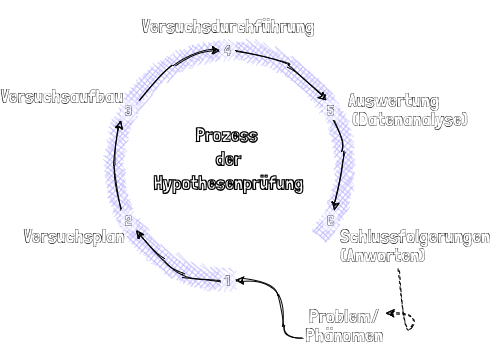
\includegraphics[width=450pt]{imgs/Hypothesen} 

}

\caption{In Anlehnung an: Reiß, S. und Sarris, V. (2012). Experimentelle Psychologie. Von der Theorie zur Praxis.}\label{fig:unnamed-chunk-18}
\end{figure}

\hypertarget{hausaufgaben}{%
\subsection{Hausaufgaben}\label{hausaufgaben}}

Lesen und Aufgaben im Olat dazu bearbeiten: Huber, Kapitel 1 - 4.2 (S. 15-98)

Außerdem bis zum nächsten Termin eine psychologische Fragestellung überlegen und im Olat eintragen.

\hypertarget{hypothesen}{%
\chapter{Hypothesen}\label{hypothesen}}

\hypertarget{organisatorisches-1}{%
\section{Organisatorisches}\label{organisatorisches-1}}

\hypertarget{semesterplan-2}{%
\subsection{Semesterplan}\label{semesterplan-2}}

\begin{tabular}[t]{rll}
\toprule
Sitzung & Datum & Sitzungstitel\\
\midrule
1 & 02.11.2020 & Warum wissenschaftliche Psychologie\\
2 & 28.11.2020
29.11.2020 & Hypothesen und der Prozess der Hypothesenprüfung\\
3 & 28.11.2020
29.11.2020 & Experimentelles Vorgehen\\
4 & 28.11.2020
29.11.2020 & Literaturrecherche\\
5 & 28.11.2020
29.11.2020 & Operationalisieren und Messen\\
\addlinespace
6 & 12.12.2020
13.12.2020 & Experimentelle Versuchspläne\\
7 & 12.12.2020
13.12.2020 & Störvariablen im Experiment\\
8 & 12.12.2020
13.12.2020 & Nicht-experimentelle Versuchspläne\\
9 & 12.12.2020
13.12.2020 & Material und Stichprobe\\
10 & 23.1.2021
24.1.2021 & Auswertung, Darstellung und Interpretation\\
\addlinespace
11 & 23.1.2021
24.1.2021 & Ethische Probleme im Versuch\\
12 & 23.1.2021
24.1.2021 & Publikationsprozess\\
13 & wird noch bekannt gegeben & Vorstellung der Gruppenarbeiten\\
14 & wird noch bekannt gegeben & Klausurvorbereitung\\
\bottomrule
\end{tabular}

\hypertarget{wiederholung}{%
\section{Wiederholung}\label{wiederholung}}

\hypertarget{alltagspsychologie}{%
\subsection{Alltagspsychologie}\label{alltagspsychologie}}

\begin{itemize}
\item
  intuitive Entscheidungsmethoden der Alltagspsychologie

  \begin{itemize}
  \item
    Fehler in der Wahrnehmung von Informationen (z.B. `Fehlwahrnehmungen', selektive Aufmerksamkeit,\ldots)
  \item
    Fehler in der Bewertung von Informationen (z.B. Urteilsheuristiken, `overconfidence', Korrelationen und Kausalität,\ldots)
  \item
    Fehler im Abruf von Informationen (z.B. Rückschaufehler, Bestätigungsfehler,\ldots)
  \end{itemize}
\item
  andere Methodik ist nötig um zu gültigen Schlussfolgerungen zu gelangen
\end{itemize}

\hypertarget{wissenschaftliche-psychologie-1}{%
\subsection{Wissenschaftliche Psychologie}\label{wissenschaftliche-psychologie-1}}

\begin{itemize}
\item
  Grundbegriffe wissenschaftlich-psychologischer Methodik

  \begin{itemize}
  \item
    Phänomen, Theorie, Modell
  \item
    Fragestellung, Hypothesen, Variablen
  \end{itemize}
\item
  Kritischer Rationalismus als normative Wisssenschaftstheorie
\item
  Prozess der Hypothesentestung als wissenschaftliche Methode der Wahl
\end{itemize}

\hypertarget{hypothesen-1}{%
\section{Hypothesen}\label{hypothesen-1}}

\hypertarget{wie-luxe4uft-der-prozess-der-hypothesenpruxfcfung-ab}{%
\subsection{Wie läuft der Prozess der Hypothesenprüfung ab?}\label{wie-luxe4uft-der-prozess-der-hypothesenpruxfcfung-ab}}

\begin{figure}

{\centering 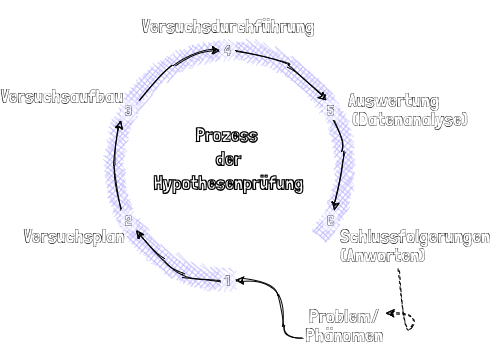
\includegraphics[width=0.5\linewidth]{imgs/Hypothesen} 

}

\caption{In Anlehnung an @reissExperimentellePsychologieTheorie2012}\label{fig:unnamed-chunk-20}
\end{figure}

\begin{cols}

\begin{col}{0.30\textwidth}

\begin{center}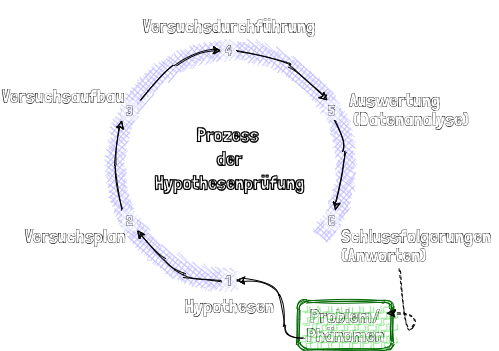
\includegraphics[width=150pt]{imgs/hypothesen_1} \end{center}

\end{col}

\begin{col}{0.68\textwidth}

\textbf{Experiment zur Ankerheuristik} \emph{Problem/Phänomen:}

Alltagsbeobachtung: Wenn man etwas nicht weiß, orientiert man sich oft an dem, was andere sagen.

\emph{Fragen:}

\begin{itemize}
\tightlist
\item
  Was ist die Ursache dafür?
\item
  Wie beeinflusst uns das Urteil anderer?
\item
  In welche Richtung wird unser Urteil verzerrt?
\item
  Spielt es eine Rolle, wer etwas sagt?
\item
  Wie gut können wir schätzen?
\item
  Welche psychischen Mechanismen spielen beim Schätzen eine Rolle?
\item
  Was ist der „Sinn" dieses „Urteilsfehlers"?
\item
  \ldots{}
\end{itemize}

\end{col}

\end{cols}

\begin{cols}

\begin{col}{0.30\textwidth}

\begin{center}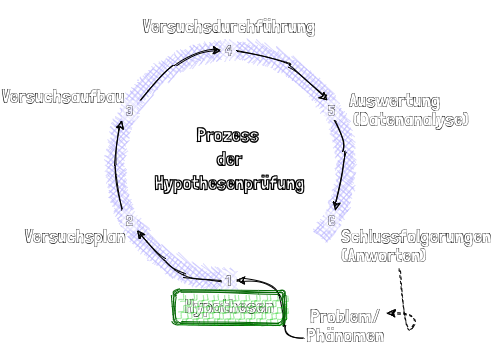
\includegraphics[width=150pt]{imgs/hypothesen_2} \end{center}

\end{col}

\begin{col}{0.68\textwidth}

\textbf{Experiment zur Ankerheuristik} \emph{Theorie:}

Beim Schätzen orientieren sich Personen oft an Heuristiken.\\
Die Ankerheuristik ist eine Urteilsheuristik, bei der sich das Urteil an einem willkürlichen „Anker" orientiert. Die Folge ist eine systematische Verzerrung in Richtung des Ankers \citep{kahnemanThinkingFastSlow2012}.\\
Laien orientieren sich bei ihren alltagswissenschaftlichen Annahmen oft an Autoritäten. Die Folge ist eine Verzerrung von Urteilen in Richtung des Urteils einer anerkannten Autorität \citep{huberPsychologischeExperiment2019}.

\end{col}

\end{cols}

\begin{cols}

\begin{col}{0.30\textwidth}

\begin{center}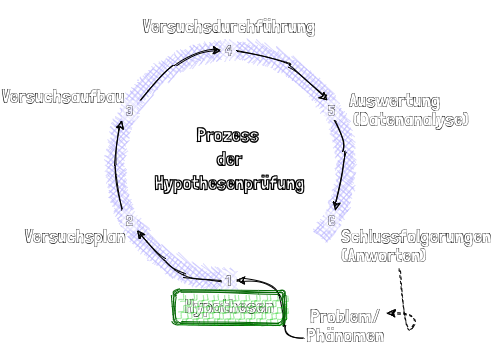
\includegraphics[width=150pt]{imgs/hypothesen_2} \end{center}

\end{col}

\begin{col}{0.68\textwidth}

\textbf{Experiment zur Ankerheuristik}

\emph{Inhaltliche Hypothesen:}

\texttt{Ankerheuristik:} Ein großer Ankerreiz führt zu einer größeren Schätzung als ein kleiner Ankerreiz.

\texttt{Autorität:} Personen verzerren ihre Schätzung stärker in Richtung des Ankers, wenn der wahrgenommene Autoritätsstatus der Ankerperson hoch ist als wenn er klein ist.

\end{col}

\end{cols}

\begin{cols}

\begin{col}{0.30\textwidth}

\begin{center}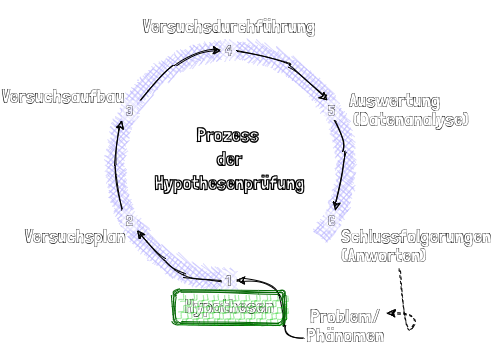
\includegraphics[width=150pt]{imgs/hypothesen_2} \end{center}

\end{col}

\begin{col}{0.68\textwidth}

\textbf{Experiment zur Ankerheuristik}

Inhaltliche Hypothesen \(\leftrightarrow\) Variablen:

\emph{Ankerheuristik:}

\texttt{Unabhängige\ Variable:} Größe des Ankerreizes

\emph{Autorität:}

\texttt{Unabhängige\ Variable:} Autoritätsstatus der Ankerperson

\emph{Urteil:}

\texttt{Abhängige\ Variable:} Schätzung

\end{col}

\end{cols}

\begin{cols}

\begin{col}{0.30\textwidth}

\begin{center}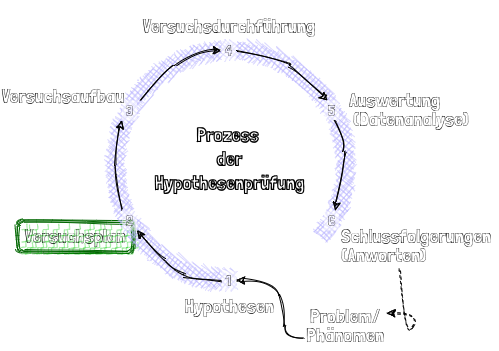
\includegraphics[width=150pt]{imgs/hypothesen_3} \end{center}

\end{col}

\begin{col}{0.68\textwidth}

\textbf{Experiment zur Ankerheuristik}

\emph{Experiment:}

\texttt{Manipulation\ der\ unabhängigen\ Variable(n)}~\\
Größe des Ankers, Autoritätsstatus `Maximiere Varianz'

\texttt{Kontrolle\ von\ Störvariablen}~\\
z.B. Vorannahmen bzgl. Experiment, Vorwissen, Intelligenz, Autoritätsgläubigkeit, Geschlecht, Müdigkeit `Kontrolliere Varianz'

\texttt{Messung\ der\ abhängigen\ Variable}~\\
Schätzung\\
`Minimiere Fehlervarianz'

\end{col}

\end{cols}

\begin{cols}

\begin{col}{0.30\textwidth}

\begin{center}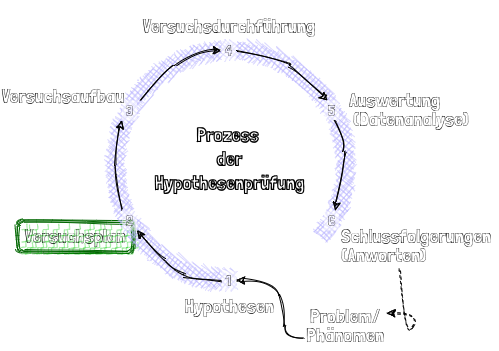
\includegraphics[width=150pt]{imgs/hypothesen_3} \end{center}

\end{col}

\begin{col}{0.68\textwidth}

\textbf{Experiment zur Ankerheuristik}

\emph{Versuchsplan (Design)} \texttt{Manipulation\ der\ unabhängigen\ Variable(n)}

Zweifaktorielles Design mit zwei „Between-Subject"-Faktoren

\begin{itemize}
\item
  \emph{Faktor 1}: Größe des Ankerreizes / Stufen: groß vs.~klein
\item
  \emph{Faktor 2}: Autoritätsstatus / Stufen: niedrig vs.~hoch
\end{itemize}

\emph{Kontrolle von Störvariablen} Durch Randomisierung wird der Einfluss von Personenmerkmalen (einigermaßen) kontrolliert

Durch zwei Verschiedene AVs wird versucht zumindest einen Teil des Effekts möglichen Vorwissens zu kontrollieren.

\emph{Messung der abhängigen Variable} Durch Eingeben der Schätzung

\end{col}

\end{cols}

\begin{cols}

\begin{col}{0.30\textwidth}

\begin{center}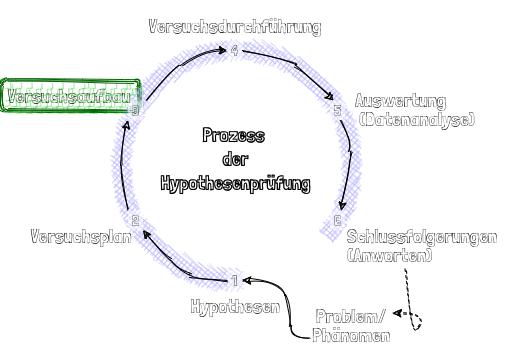
\includegraphics[width=150pt]{imgs/hypothesen_4} \end{center}

\end{col}

\begin{col}{0.68\textwidth}

\textbf{Experiment zur Ankerheuristik - NOK}

\emph{Operationalisierung}

\texttt{Unabhängige\ Variablen:} Größe des Ankerreizes groß= 200 km vs.~klein= 50 km

Autoritätsstatus niedrig= 1. Vorstand des Bayerischen Dachshundklubs vs.~hoch= ehemaliger Ministerpräsident

\texttt{Störvariablen:} VP-interne Störvariablen wurden durch Randomisierung kontrolliert.

\texttt{Abhängigen\ Variable:} Wie lang ist der Nord-Ostsee-Kanal, was schätzen Sie? \_\_\_\_ km

\end{col}

\end{cols}

\begin{cols}

\begin{col}{0.30\textwidth}

\begin{center}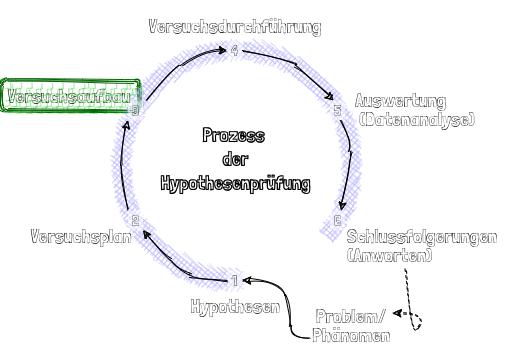
\includegraphics[width=150pt]{imgs/hypothesen_4} \end{center}

\end{col}

\begin{col}{0.68\textwidth}

\textbf{Experiment zur Ankerheuristik - Afrika}

\emph{Operationalisierung}

\texttt{Unabhängige\ Variablen:} Größe des Ankerreizes groß= 85 km vs.~klein= 25 km

Autoritätsstatus niedrig= Donald Trump vs.~hoch= Nelson Mandela

\texttt{Störvariablen:} VP-interne Störvariablen wurden durch Randomisierung kontrolliert. Heterogenes Vorwissen durch wurde unbekanntes Thema kontrolliert.

\texttt{Abhängigen\ Variable:} Wie viele Länder liegen auf dem afrikanischen Kontinent, was schätzen Sie? \_\_\_\_ Länder

\end{col}

\end{cols}

\begin{cols}

\begin{col}{0.30\textwidth}

\begin{center}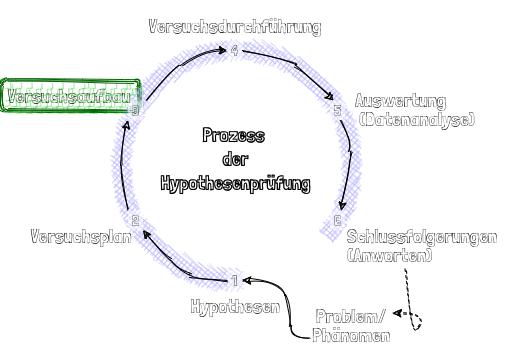
\includegraphics[width=150pt]{imgs/hypothesen_4} \end{center}

\end{col}

\begin{col}{0.68\textwidth}

\textbf{Experiment zur Ankerheuristik - Afrika}

\emph{Versuchspersonen}

Als \texttt{Ad-hoc}-Stichprobe, anfallende Stichprobe, Gelegenheitsstichprobe, aber auch manchmal treffend als Bequemlichkeitsauswahl bezeichnet man in der psychologischen Forschung eine willkürliche Untersuchung von gerade zur Verfügung stehenden Proband*Innen.(In der Regel Psychologie-Studierende)

Nachteile: Schlechte Kontrolle von Störvariablen, u.U. geringe Generalisierbarkeit

\end{col}

\end{cols}

\begin{cols}

\begin{col}{0.30\textwidth}

\begin{center}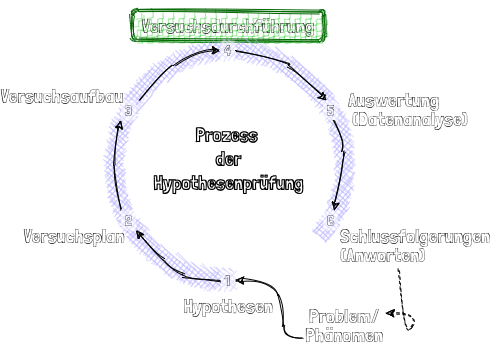
\includegraphics[width=150pt]{imgs/hypothesen_5} \end{center}

\end{col}

\begin{col}{0.68\textwidth}

\textbf{Experiment zur Ankerheuristik}

\emph{Aufklärung und Instruktionen} Nicht standardisierter verbaler Aufruf, VL umreißt Versuchsbedingungen. Standardisierter Aufgabentext bei zufällig zugeteilter Aufgabe.

\emph{Ablauf} Aufruf der Website, Ausfüllen, Abschicken

\end{col}

\end{cols}

\begin{cols}

\begin{col}{0.30\textwidth}

\begin{center}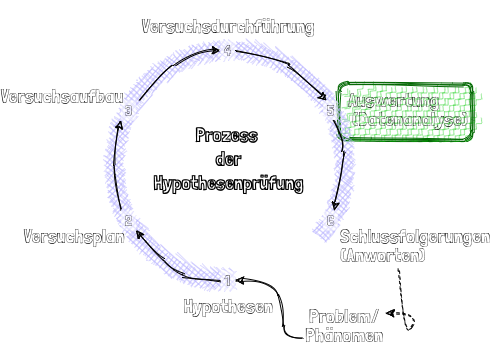
\includegraphics[width=150pt]{imgs/hypothesen_6} \end{center}

\end{col}

\begin{col}{0.68\textwidth}

\textbf{Experiment zur Ankerheuristik}

\begin{itemize}
\item
  Schritt 1: Datenaufbereitung Schätzungen von Server abfragen, Ausreißer entfernen.
\item
  Schritt 2: Überprüfung der Voraussetzungen

  \begin{itemize}
  \tightlist
  \item
    Normalverteiltheit
  \item
    Varianzhomogenität
  \item
    Unabhängigkeit
  \end{itemize}
\item
  Schritt 3: Deskriptive und Inferenzstatistik

  \begin{itemize}
  \tightlist
  \item
    Mittelwerte, Standardabweichungen . . .
  \item
    Zweifaktorielle Varianzanalyse
  \end{itemize}
\end{itemize}

\end{col}

\end{cols}

\begin{cols}

\begin{col}{0.30\textwidth}

\begin{center}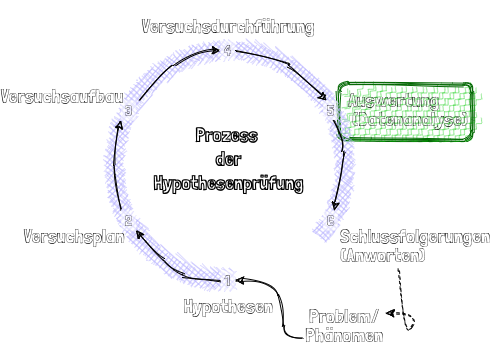
\includegraphics[width=150pt]{imgs/hypothesen_6} \end{center}

\end{col}

\begin{col}{0.68\textwidth}

\textbf{Experiment zur Ankerheuristik}

\begin{center}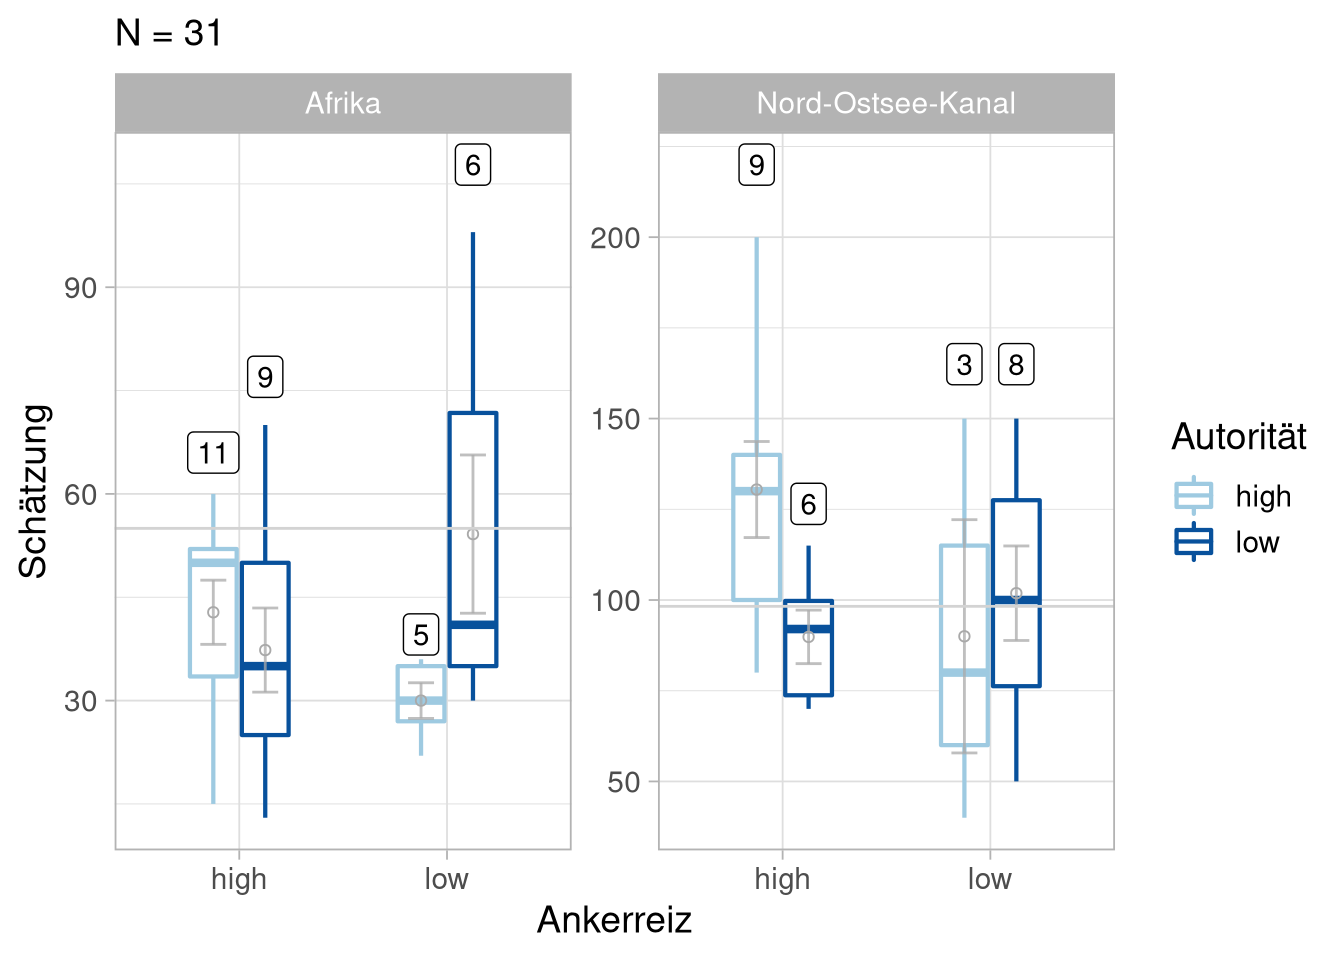
\includegraphics[width=500pt]{Versuchsplanung_WS20_files/figure-latex/unnamed-chunk-33-1} \end{center}

\end{col}

\end{cols}

\hypertarget{nok}{%
\subsubsection{NOK}\label{nok}}

\begin{tabular}[t]{lrrrrr}
\toprule
Effect & DFn & DFd & F & p & ges\\
\midrule
anchor & 1 & 22 & 0.319791 & 0.5774558 & 0.0143277\\
authority & 1 & 22 & 1.838841 & 0.1888431 & 0.0771363\\
anchor:authority & 1 & 22 & 2.749719 & 0.1114632 & 0.1111010\\
\bottomrule
\end{tabular}

Es gab weder einen signifikanten Haupteffekt des Faktors Größe des Ankerreizes (\(F_{1,22}=0.32, p = 0.32, \hat{\eta}^2 =0.014\))

noch des Autoritätsstatus (\(F_{1,22}=1.84, p = 1.839, \hat{\eta}^2 =0.077\)).

Auch die Interaktion wurde nicht signifikant\\
(\(F_{1,22}=2.75, p = 2.75, \hat{\eta}^2 =0.111\)).

\hypertarget{afrika}{%
\subsubsection{Afrika}\label{afrika}}

\begin{tabular}[t]{lrrrrr}
\toprule
Effect & DFn & DFd & F & p & ges\\
\midrule
anchor & 1 & 27 & 0.1144927 & 0.7377033 & 0.0042226\\
authority & 1 & 27 & 0.5764964 & 0.4542672 & 0.0209054\\
anchor:authority & 1 & 27 & 4.5548807 & 0.0420580 & 0.1443479\\
\bottomrule
\end{tabular}

Es gab weder einen signifikanten Haupteffekt des Faktors Größe des Ankerreizes (\(F_{1,27}=0.11, p = 0.114, \hat{\eta}^2 =0.004\))
noch des Autoritätsstatus\\
(\(F_{1,27}=0.58, p = 0.576, \hat{\eta}^2 =0.021\)).

Die Interaktion ist aber signifikant geworden\\
(\(F_{1,27}=4.55, p = 4.555, \hat{\eta}^2 =0.144\)).

\begin{cols}

\begin{col}{0.30\textwidth}

\begin{center}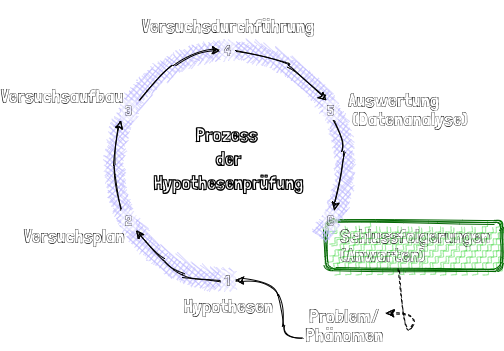
\includegraphics[width=150pt]{imgs/hypothesen_7} \end{center}

\end{col}

\begin{col}{0.68\textwidth}

\textbf{Experiment zur Ankerheuristik}

\emph{Inhaltliche Hypothesen}

\texttt{Ankerheuristik:} Ein großer Ankerreiz führt zu einer größeren Schätzung als ein kleiner Ankerreiz.

\(\rightarrow\) hat sich nicht bewährt

\texttt{Autorität:} Personen verzerren ihre Schätzung stärker in Richtung des Ankers, wenn der wahrgenommene Autoritätsstatus der Ankerperson hoch ist als wenn er klein ist

\(\rightarrow\) hat sich nicht bewährt

\begin{quote}
\begin{itemize}
\tightlist
\item
  Aber zumindest im Afrika-Fall wurde die Interaktion signifikant, was darauf hindeutet, dass es ein nicht rein additives Zusammenwirken von Anker und Autoritätsreiz gibt.
\end{itemize}
\end{quote}

\end{col}

\end{cols}

\textbf{Experiment zur Ankerheuristik} Weder der Einfluss der Ankerheuristik, noch die Autoritätsverzerrung konnte so richtig gezeigt werden. Warum?

Ist die Hypothese unbrauchbar, oder\ldots{}

\begin{itemize}
\item
  brauchen wir einfach eine größere Testpower? (Effektgröße, N, Fehler)

  \begin{itemize}
  \item
    Lösung:

    \begin{itemize}
    \tightlist
    \item
      Vergrößerung der Primärvarianz (Effekt\(\uparrow\)),
    \item
      Verkleinern des Messfehlers (N\(\uparrow\), Fehler\(\downarrow\))
    \end{itemize}
  \end{itemize}
\item
  haben wir irgendwelche Störvariablen (z.B. Vorwissen, technische Probleme) übersehen?

  \begin{itemize}
  \item
    Lösung:

    \begin{itemize}
    \tightlist
    \item
      Kontrolle der Störvariablen (z.B. Vorwissen, Vorurteile, usw. abfragen und ausbalancieren)
    \end{itemize}
  \end{itemize}
\end{itemize}

\hypertarget{hypothesen-2}{%
\subsection{Hypothesen}\label{hypothesen-2}}

\begin{itemize}
\item
  Definition „Hypothese"
\item
  Wie kommt man zu Hypothesen?

  \begin{itemize}
  \tightlist
  \item
    Unsystematische vs.~systematische Ansätze
  \item
    Rolle von Induktion und Deduktion
  \item
    Häufige Fehler bei der Generierung von Hypothesen
  \end{itemize}
\item
  Wie überprüft man Hypothesen (nicht)?

  \begin{itemize}
  \tightlist
  \item
    Ungültige „Beweise"
  \item
    Prozess der wissenschaftlichen Hypothesenprüfung
  \end{itemize}
\item
  Bewertung von Hypothesen und deren Überprüfung

  \begin{itemize}
  \tightlist
  \item
    Vorbedingungen für Überprüfbarkeit
  \item
    Qualitätskriterien für Hypothesen und deren Überprüfung
  \end{itemize}
\end{itemize}

\hypertarget{definition-hypothese}{%
\subsection{Definition Hypothese:}\label{definition-hypothese}}

\begin{itemize}
\tightlist
\item
  Kurzversion: Eine Hypothese ist eine vermutete Antwort auf eine Frage.
\item
  Langversion: Eine Hypothese ist eine beliebige Aussage, die man provisorisch für bestimmte Zwecke als wahr annimmt, auch wenn man nicht oder zumindest nicht genau weiß, ob sie wirklich wahr oder falsch ist.
\end{itemize}

\hypertarget{zweck-von-hypothesen}{%
\subsubsection{Zweck von Hypothesen:}\label{zweck-von-hypothesen}}

\begin{itemize}
\tightlist
\item
  Hypothesen ermöglichen Vorhersagen im Rahmen einer Hypothesenprüfung.
\end{itemize}

\hypertarget{vorsicht}{%
\subsubsection{Vorsicht!}\label{vorsicht}}

\begin{itemize}
\tightlist
\item
  inhaltliche Hypothesen \(\neq\) statistische Hypothesen
\end{itemize}

\hypertarget{wie-kommt-man-zu-hypothesen}{%
\subsection{Wie kommt man zu Hypothesen?}\label{wie-kommt-man-zu-hypothesen}}

\hypertarget{unsystematischer-ansatz}{%
\subsubsection{Unsystematischer Ansatz:}\label{unsystematischer-ansatz}}

\begin{itemize}
\tightlist
\item
  Alltagspsychologie
\item
  Neugier, Intuition, Kreativität
\item
  Diskussion mit Kollegen
\item
  Zufall
\end{itemize}

\hypertarget{systematischer-ansatz}{%
\subsubsection{Systematischer Ansatz:}\label{systematischer-ansatz}}

\begin{itemize}
\tightlist
\item
  Sammlung von Fallbeschreibungen und Verallgemeinerung (Induktion)
\item
  Explorative Studien, Erkundungsexperimente, Umfragen
\item
  Replikation von bekannten Untersuchungen
\item
  Klärung von widersprüchlichen Ergebnissen
\item
  Ableitung aus Theorien (Deduktion)
\end{itemize}

\hypertarget{exkurs-induktion-deduktion}{%
\subsection{Exkurs Induktion \& Deduktion}\label{exkurs-induktion-deduktion}}

Wie kommt man zu Hypothesen/Theorien?

\begin{figure}

{\centering 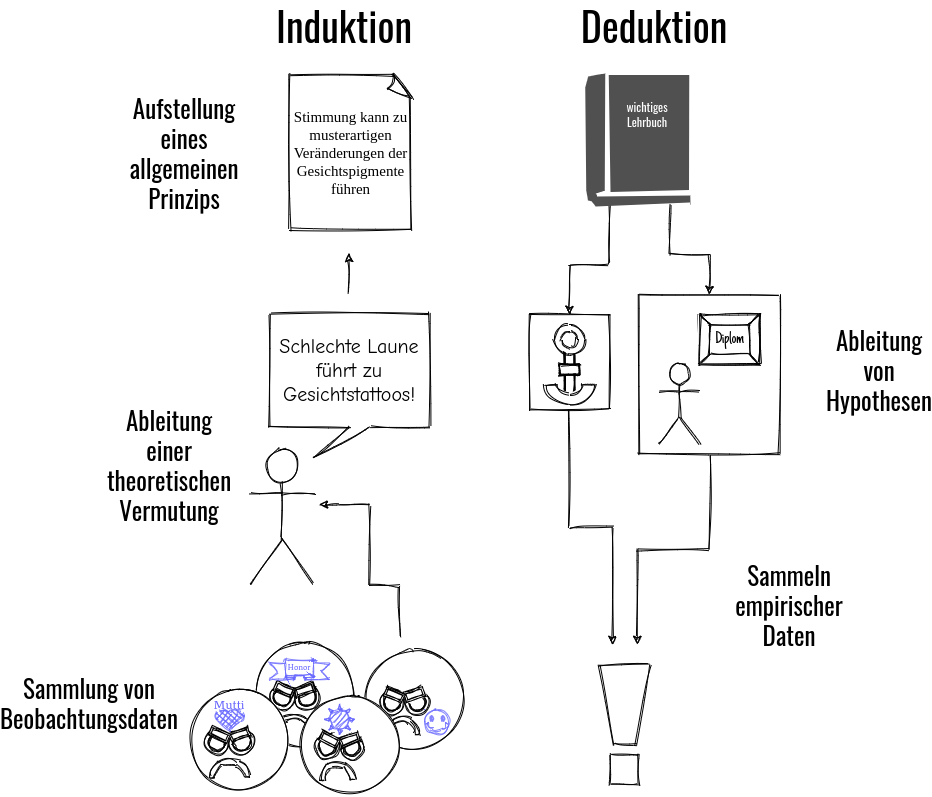
\includegraphics[width=200pt]{imgs/InduDedu} 

}

\caption{In Anlehnung an @reissExperimentellePsychologieTheorie2012}\label{fig:unnamed-chunk-38}
\end{figure}

\hypertarget{wie-uxfcberpruxfcft-man-hypothesen-nicht}{%
\subsection{Wie überprüft man Hypothesen (nicht)?}\label{wie-uxfcberpruxfcft-man-hypothesen-nicht}}

Mit `Methodik' der Alltagspsychologie \(\rightarrow\) erste Sitzung

\hypertarget{wie-luxe4uft-der-prozess-der-hypothesenpruxfcfung-ab-1}{%
\subsection{Wie läuft der Prozess der Hypothesenprüfung ab?}\label{wie-luxe4uft-der-prozess-der-hypothesenpruxfcfung-ab-1}}

\begin{center}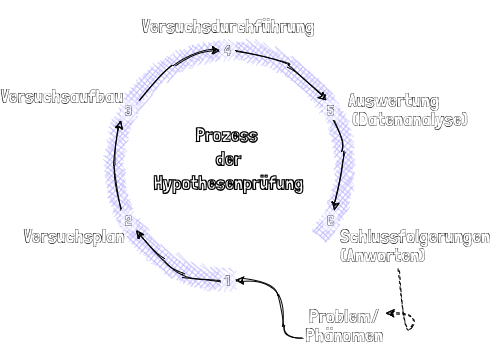
\includegraphics[width=200pt]{imgs/Hypothesen} \end{center}

\hypertarget{bewertung-von-hypothesen-und-deren-uxfcberpruxfcfung}{%
\subsection{Bewertung von Hypothesen und deren Überprüfung:}\label{bewertung-von-hypothesen-und-deren-uxfcberpruxfcfung}}

Vorbedingungen:

\begin{itemize}
\tightlist
\item
  Widerspruchsfreiheit
\item
  Kritisierbarkeit (Falsifizierbarkeit)
\item
  Operationalisierbarkeit
\item
  Aufstellung der Hypothese VOR der Überprüfung
\end{itemize}

Qualitätskriterien:

\begin{itemize}
\tightlist
\item
  Möglichst wenig Annahmen (Occam's Razor)
\item
  Möglichst strenge Prüfung (Bewährungsgrad, Bewährungsbereich)
\end{itemize}

\hypertarget{operationalisierung-messbarmachung}{%
\subsection{Operationalisierung = Messbarmachung}\label{operationalisierung-messbarmachung}}

Welche Rolle spielt die Operationalisierung von Hypothesen für deren Überprüfung? Beispiel: Welchen Einfluss hat Ängstlichkeit auf Lernen?

\begin{center}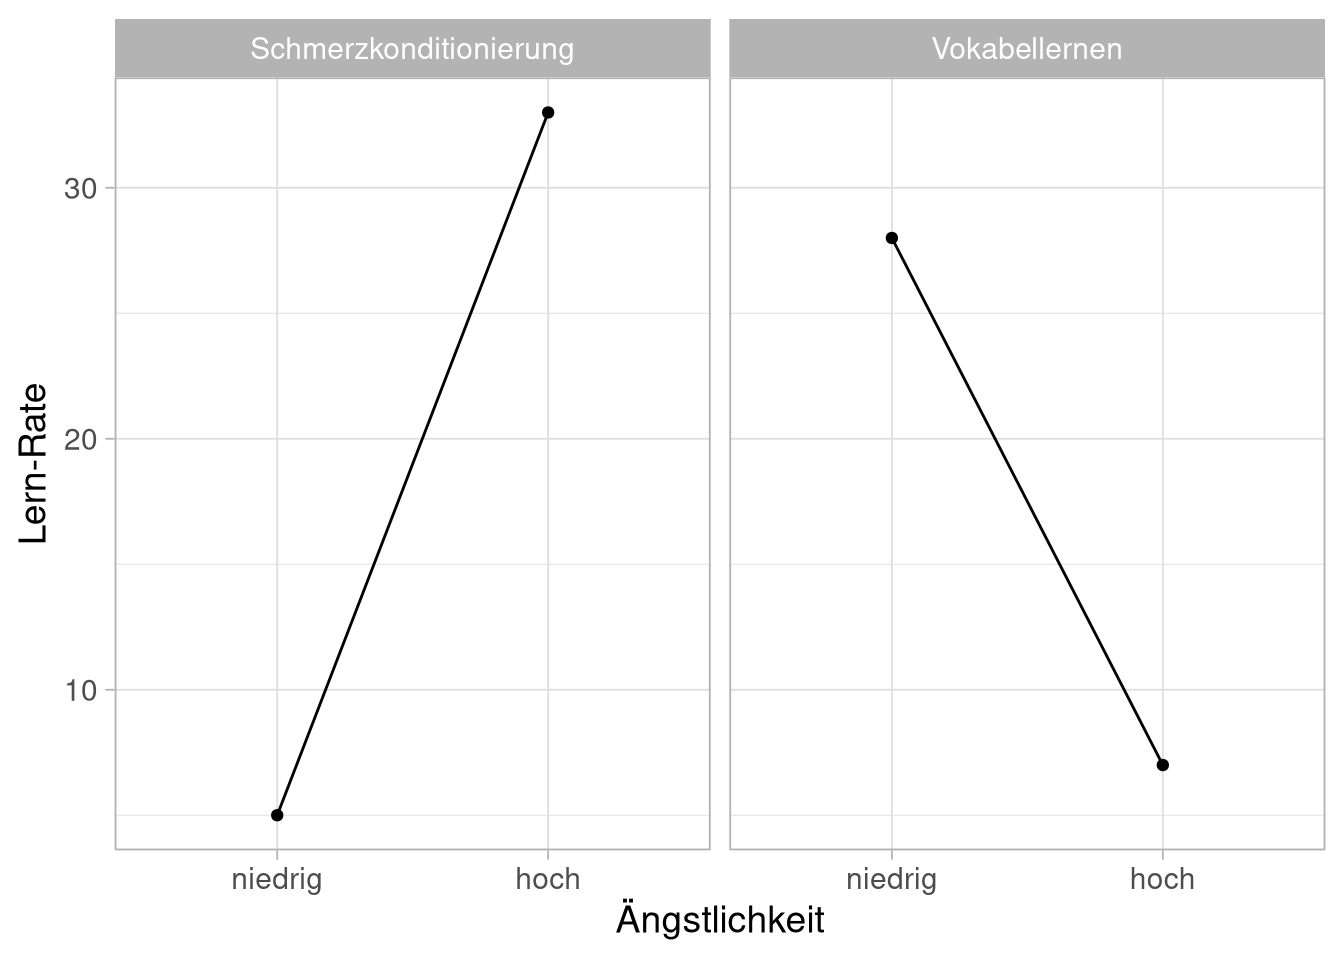
\includegraphics[width=200pt]{Versuchsplanung_WS20_files/figure-latex/lernen-1} \end{center}

Welche Rolle spielt die Operationalisierung von Hypothesen für deren Überprüfung?

Art und Weise der Operationalisierung der theoretischen Konzepte (Lernen) \(\rightarrow\) Geltungsbereich des erhobenen experimentellen Befundes (Konditionierung vs.~Schule)

\hypertarget{bewertung-von-hypothesen-und-deren-uxfcberpruxfcfung-1}{%
\subsection{Bewertung von Hypothesen und deren Überprüfung:}\label{bewertung-von-hypothesen-und-deren-uxfcberpruxfcfung-1}}

Vorbedingungen:

\begin{itemize}
\tightlist
\item
  Widerspruchsfreiheit
\item
  Kritisierbarkeit (Falsifizierbarkeit)
\item
  Operationalisierbarkeit
\item
  Aufstellung der Hypothese VOR der Überprüfung
\end{itemize}

Qualitätskriterien:

\begin{itemize}
\tightlist
\item
  Möglichst wenig Annahmen (Occam's Razor)
\item
  Möglichst strenge Prüfung (Bewährungsgrad, Bewährungsbereich)
\end{itemize}

\hypertarget{aufstellung-der-hypothese-vor-der-uxfcberpruxfcfung}{%
\subsection{Aufstellung der Hypothese VOR der Überprüfung}\label{aufstellung-der-hypothese-vor-der-uxfcberpruxfcfung}}

\begin{cols}

\begin{col}{0.30\textwidth}

\end{col}

\begin{col}{0.68\textwidth}

Ein Bogenschütze, der sein Ziel nach dem Schießen erklärt, trifft zwar immer, ist aber nicht unbedingt gut im Bogenschießen.

\end{col}

\end{cols}

\hypertarget{occams-razor}{%
\subsection{Occam's Razor}\label{occams-razor}}

\begin{cols}

\begin{col}{0.30\textwidth}

\end{col}

\begin{col}{0.68\textwidth}

\emph{Numquam ponenda est pluralitas sine necessitate}

\end{col}

\end{cols}

Ungefähr-Übersetzung:

Eine Mehrheit darf nie ohne Not zugrunde gelegt werden.

\hypertarget{ausblick}{%
\section{Ausblick}\label{ausblick}}

\begin{itemize}
\tightlist
\item
  Grundidee des Experimentes und Typen von Experimenten
\item
  Vertiefung: unabhängige und abhängige Variablen
\item
  Reiz-, Reaktions-, Organismusvariablen
\item
  Störvariablen: Konfundierung vs.~Kontrolltechniken
\item
  Datenfluktuation: Max-Kon-Min-Prinzip
\item
  Interne und externe Validität
\end{itemize}

\hypertarget{experimentelles-vorgehen-und-kausalschluxfcsse}{%
\chapter{Experimentelles Vorgehen und Kausalschlüsse}\label{experimentelles-vorgehen-und-kausalschluxfcsse}}

\hypertarget{organisatorisches-2}{%
\section{Organisatorisches}\label{organisatorisches-2}}

\hypertarget{semesterplan-3}{%
\subsection{Semesterplan}\label{semesterplan-3}}

\begin{tabular}[t]{rll}
\toprule
Sitzung & Datum & Sitzungstitel\\
\midrule
1 & 02.11.2020 & Warum wissenschaftliche Psychologie\\
2 & 28.11.2020
29.11.2020 & Hypothesen und der Prozess der Hypothesenprüfung\\
3 & 28.11.2020
29.11.2020 & Experimentelles Vorgehen\\
4 & 28.11.2020
29.11.2020 & Literaturrecherche\\
5 & 28.11.2020
29.11.2020 & Operationalisieren und Messen\\
\addlinespace
6 & 12.12.2020
13.12.2020 & Experimentelle Versuchspläne\\
7 & 12.12.2020
13.12.2020 & Störvariablen im Experiment\\
8 & 12.12.2020
13.12.2020 & Nicht-experimentelle Versuchspläne\\
9 & 12.12.2020
13.12.2020 & Material und Stichprobe\\
10 & 23.1.2021
24.1.2021 & Auswertung, Darstellung und Interpretation\\
\addlinespace
11 & 23.1.2021
24.1.2021 & Ethische Probleme im Versuch\\
12 & 23.1.2021
24.1.2021 & Publikationsprozess\\
13 & wird noch bekannt gegeben & Vorstellung der Gruppenarbeiten\\
14 & wird noch bekannt gegeben & Klausurvorbereitung\\
\bottomrule
\end{tabular}

\hypertarget{wiederholung-1}{%
\section{Wiederholung}\label{wiederholung-1}}

\hypertarget{prozess-der-hypothesenpruxfcfung}{%
\subsection{Prozess der Hypothesenprüfung}\label{prozess-der-hypothesenpruxfcfung}}

\begin{figure}

{\centering 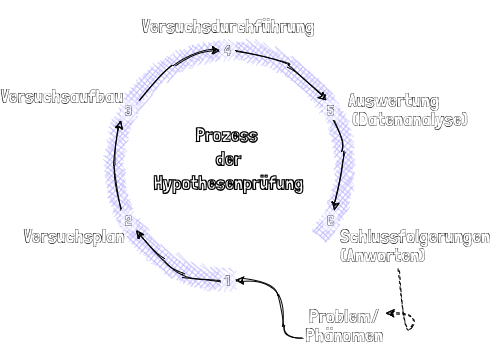
\includegraphics[width=0.5\linewidth]{imgs/Hypothesen} 

}

\caption{In Anlehnung an @reissExperimentellePsychologieTheorie2012}\label{fig:unnamed-chunk-45}
\end{figure}

\hypertarget{hypothesen-3}{%
\subsection{Hypothesen}\label{hypothesen-3}}

\begin{itemize}
\tightlist
\item
  Definition „Hypothese``
\item
  Wie kommt man zu Hypothesen?

  \begin{itemize}
  \tightlist
  \item
    Unsystematische vs.~systematische Ansätze
  \item
    Rolle von Induktion und Deduktion
  \item
    Häufige Fehler bei der Generierung von Hypothesen
  \end{itemize}
\item
  Wie überprüft man Hypothesen (nicht)?

  \begin{itemize}
  \tightlist
  \item
    Ungültige „Beweise``
  \item
    Prozess der wissenschaftlichen Hypothesenprüfung
  \end{itemize}
\item
  Bewertung von Hypothesen und deren Überprüfung

  \begin{itemize}
  \tightlist
  \item
    Vorbedingungen für Überprüfbarkeit
  \item
    Qualitätskriterien für Hypothesen und deren Überprüfung
  \end{itemize}
\end{itemize}

\hypertarget{grundidee-des-experimentierens}{%
\section{Grundidee des Experimentierens}\label{grundidee-des-experimentierens}}

\hypertarget{welche-merkmale-definieren-ein-experiment}{%
\subsection{Welche Merkmale definieren ein Experiment}\label{welche-merkmale-definieren-ein-experiment}}

\begin{enumerate}
\def\labelenumi{\arabic{enumi}.}
\item
  Manipulation mindestens einer unabhängigen Variable
\item
  Kontrolle von (möglichst allen relevanten) Störvariablen
\item
  Messung mindestens einer abhängigen Variable
\end{enumerate}

\hypertarget{kausalituxe4t}{%
\subsection{Kausalität}\label{kausalituxe4t}}

\hypertarget{warum-lassen-nicht-experimentelle-studien-keinen-kausalschluss-zu}{%
\subsubsection{Warum lassen nicht-experimentelle Studien keinen Kausalschluss zu?}\label{warum-lassen-nicht-experimentelle-studien-keinen-kausalschluss-zu}}

\[\text{Kausalität} = \text{Ursache-Wirkungs-Beziehung}\]

\hypertarget{beispiel}{%
\subsubsection{Beispiel:}\label{beispiel}}

\begin{cols}

\begin{col}{0.30\textwidth}

\begin{center}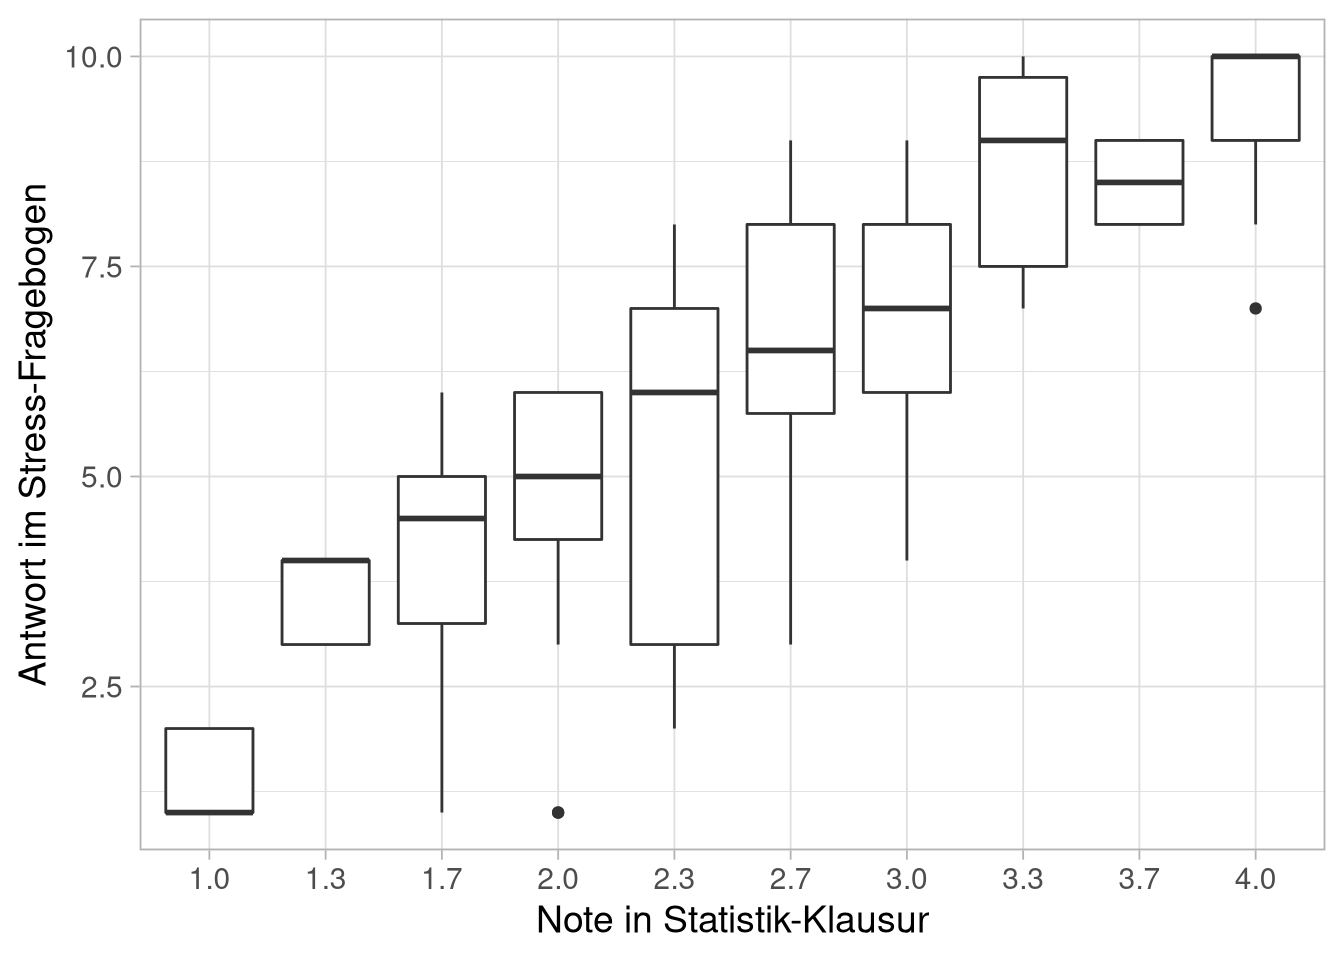
\includegraphics[width=150pt]{Versuchsplanung_WS20_files/figure-latex/unnamed-chunk-47-1} \end{center}

\end{col}

\begin{col}{0.68\textwidth}

Ein Forscher beobachtet, dass Studierende, die hohe Werte in einem Stress-
Fragebogen angeben, schlechte Leistungen in der Statistik-Klausur zeigen und
dass Studierende, die niedrige Werte im Stress-Fragebogen angeben, gute
Leistungen in der Statistik-Klausur zeigen.

\end{col}

\end{cols}

\hypertarget{beispiel-zu-kausalschluxfcssen}{%
\subsection{Beispiel zu Kausalschlüssen}\label{beispiel-zu-kausalschluxfcssen}}

\hypertarget{warum-lassen-nicht-experimentelle-studien-keinen-kausalschluss-zu-1}{%
\subsubsection{Warum lassen nicht-experimentelle Studien keinen Kausalschluss zu?}\label{warum-lassen-nicht-experimentelle-studien-keinen-kausalschluss-zu-1}}

\textbf{Mögliche `Schlussfolgerung' aus Ergebnissen:}

\begin{center}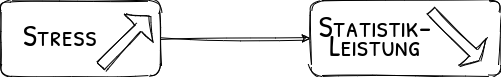
\includegraphics[width=200pt]{imgs/direct_causality} \end{center}

Stress vermindert die Prüfungsleistung in Statistik.

\begin{center}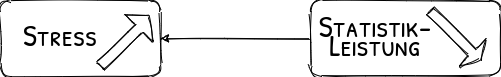
\includegraphics[width=200pt]{imgs/reverse_causality} \end{center}

Wer schlecht in Statistik ist, den stresst das Lernen für Statistik-Klausuren.

\begin{center}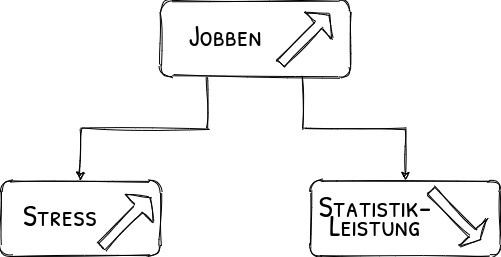
\includegraphics[width=200pt]{imgs/confound_causality} \end{center}

Wer viel jobbt ist sowohl schlechter in Statistik, als auch im allgemeinen gestresster.

\begin{center}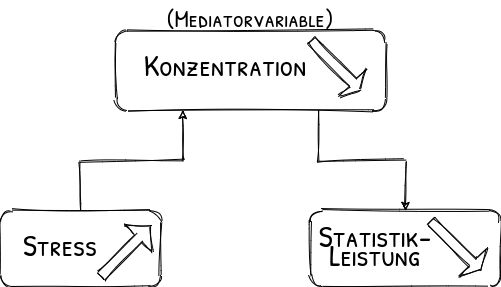
\includegraphics[width=200pt]{imgs/mediator_causality} \end{center}

Stress verschlechtert die Konzentration.

Schlechte Konzentration beeinträchtigt die Leistung

\begin{center}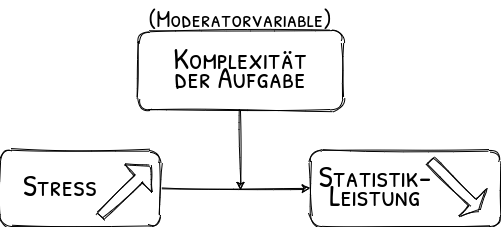
\includegraphics[width=200pt]{imgs/moderator_causality} \end{center}

Stress beeinflusst nur die Leistung bei besonders komplexen Aufgaben, die dann aber auch die meisten Punkte bringen.

\hypertarget{beispiel-zu-kausalschluxfcssen-1}{%
\subsection{Beispiel zu Kausalschlüssen}\label{beispiel-zu-kausalschluxfcssen-1}}

\hypertarget{warum-lassen-nicht-experimentelle-studien-keinen-kausalschluss-zu-2}{%
\subsubsection{Warum lassen nicht-experimentelle Studien keinen Kausalschluss zu?}\label{warum-lassen-nicht-experimentelle-studien-keinen-kausalschluss-zu-2}}

\begin{figure}

{\centering 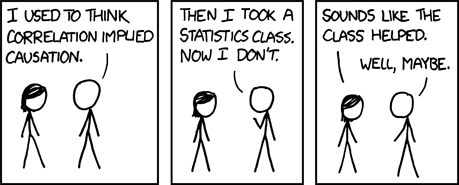
\includegraphics[width=133.333333333333pt]{imgs/correlation} 

}

\caption{Abbildung unter CC-BY-NC-Lizenz, Quelle: [xkcd](https://xkcd.com/552/)}\label{fig:unnamed-chunk-55}
\end{figure}

\begin{figure}

{\centering 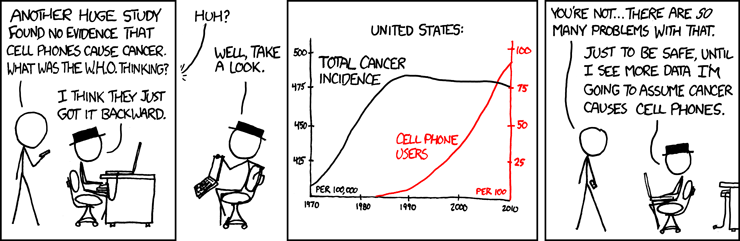
\includegraphics[width=216.666666666667pt]{imgs/cell_phones} 

}

\caption{Abbildung unter CC-BY-NC-Lizenz, Quelle: [xkcd](https://xkcd.com/925/)}\label{fig:unnamed-chunk-57}
\end{figure}

\hypertarget{luxf6sung-experiment}{%
\subsection{Lösung: Experiment}\label{luxf6sung-experiment}}

\hypertarget{fall-von-eben}{%
\subsubsection{Fall von eben}\label{fall-von-eben}}

\begin{cols}

\begin{col}{0.30\textwidth}

\begin{center}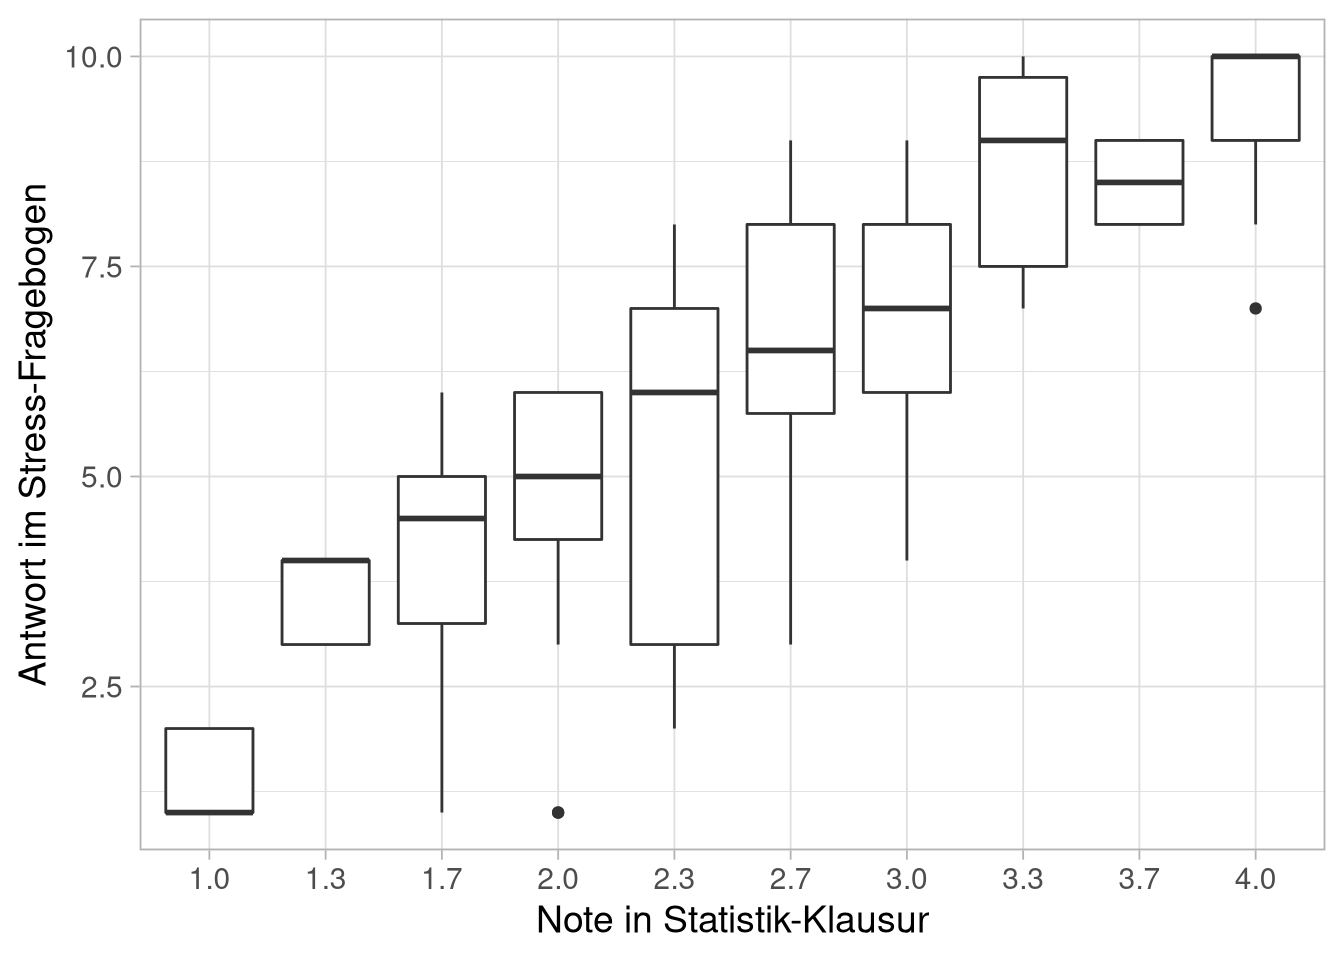
\includegraphics[width=150pt]{Versuchsplanung_WS20_files/figure-latex/unnamed-chunk-59-1} \end{center}

\end{col}

\begin{col}{0.68\textwidth}

Ein Forscher beobachtet, dass Studierende, die hohe Werte in einem Stress-
Fragebogen angeben, schlechte Leistungen in der Statistik-Klausur zeigen und
dass Studierende, die niedrige Werte im Stress-Fragebogen angeben, gute
Leistungen in der Statistik-Klausur zeigen.

\end{col}

\end{cols}

\hypertarget{manipuliere-unabhuxe4ngige-variablen}{%
\subsubsection{Manipuliere unabhängige Variablen}\label{manipuliere-unabhuxe4ngige-variablen}}

\begin{itemize}
\tightlist
\item
  Stress

  \begin{itemize}
  \tightlist
  \item
    Niedrig: Vor dem Test entspannen
  \item
    Hoch: Vor dem Test Vortrag halten
  \end{itemize}
\item
  Komplexität der Aufgabe

  \begin{itemize}
  \tightlist
  \item
    Niedrig: Konzentrationsaufgaben (d2 durchstreichen)
  \item
    Hoch: Statistik-Aufgaben
  \end{itemize}
\end{itemize}

\hypertarget{kontrolliere-stuxf6rvariablen}{%
\subsubsection{Kontrolliere Störvariablen}\label{kontrolliere-stuxf6rvariablen}}

\begin{itemize}
\item
  Jobben (in h/Woche) --- randomisieren
\item
  Statistik-Kenntnisse (Note im 1. Semester) --- randomisieren
\item
  Geschlecht (w/m) --- parallelisieren (Blockbildung)
\item
  Reihenfolge der Aufgaben --- Ausbalancierung
\end{itemize}

\hypertarget{messe-abhuxe4ngige-variablen}{%
\subsubsection{Messe abhängige Variablen}\label{messe-abhuxe4ngige-variablen}}

\begin{itemize}
\tightlist
\item
  Leistung

  \begin{itemize}
  \tightlist
  \item
    Anzahl korrekte Lösungen
  \item
    Antwortlatenzen
  \end{itemize}
\end{itemize}

\hypertarget{design}{%
\subsubsection{Design:}\label{design}}

\begin{tikzpicture}
\tikzset{
    mytext/.style={text width=7em,align=center},
    mylabel/.style={text width=7em,align=center, font=\footnotesize}
}
  \node[mylabel] at (2.5,7.75) {niedrig};
  \node[mylabel] at (6,7.75) {hoch};
  \node[mylabel] at (0,6) {niedrig};
  \node[mylabel] at (0,2.5) {hoch};
  \node[mytext] at (-0.5,4.25) {Stress};
  \node[mytext] at (4.25,8) {Komplexität};
  \node[mylabel] at(9.5, 4.25) {Kreuzung der \newline Faktoren: \newline $2\cdot 2=4$ Zellen \newline};
  \draw (1,1) -- (4,1) -- (4,4) -- (1,4) -- (1,1);
  \draw (4.5,4.5) -- (7.5,4.5) -- (7.5,7.5) -- (4.5,7.5) -- (4.5,4.5);
  \draw (1,4.5) -- (4,4.5) -- (4,7.5) -- (1,7.5) -- (1,4.5);
  \draw (4.5,1) -- (4.5,4) -- (7.5,4) -- (7.5,1) -- (4.5,1);
\end{tikzpicture}

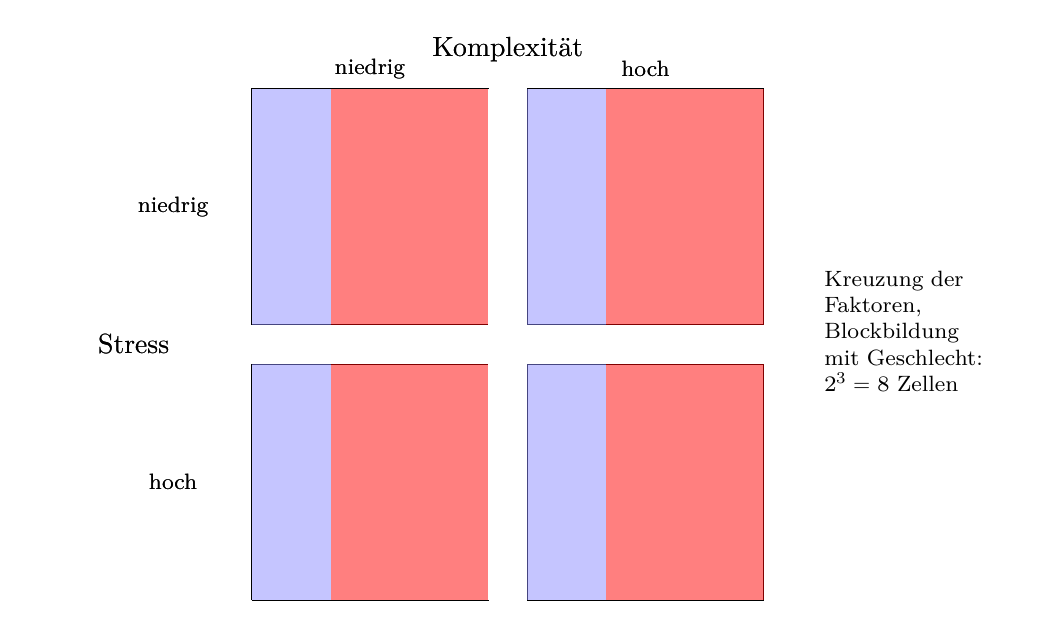
\begin{tikzpicture}
\tikzset{
    mytext/.style={text width=7em,align=center},
    mylabel/.style={text width=7em,align=center, font=\footnotesize}
}
  \node[mylabel] at (2.5,7.75) {niedrig};
  \node[mylabel] at (6,7.75) {hoch};
  \node[mylabel] at (0,6) {niedrig};
  \node[mylabel] at (0,2.5) {hoch};
  \node[mytext] at (-0.5,4.25) {Stress};
  \node[mytext] at (4.25,8) {Komplexität};
  <!-- \draw (1,1) -- (4,1) -- (4,4) -- (1,4) -- (1,1); -->
  <!-- \draw (4.5,4.5) -- (7.5,4.5) -- (7.5,7.5) -- (4.5,7.5) -- (4.5,4.5); -->
  <!-- \draw (1,4.5) -- (4,4.5) -- (4,7.5) -- (1,7.5) -- (1,4.5); -->
  <!-- \draw (4.5,1) -- (4.5,4) -- (7.5,4) -- (7.5,1) -- (4.5,1); -->
  \draw (1,1) -- (4,1) -- (4,4) -- (1,4) -- (1,1);
  \draw (4.5,4.5) -- (7.5,4.5) -- (7.5,7.5) -- (4.5,7.5) -- (4.5,4.5);
  \draw (1,4.5) -- (4,4.5) -- (4,7.5) -- (1,7.5) -- (1,4.5);
  \draw (4.5,1) -- (4.5,4) -- (7.5,4) -- (7.5,1) -- (4.5,1);
  \fill [Red, opacity=.5] (2,1) rectangle (4,7.5);
  \fill [Red, opacity=.5] (5.5,1) rectangle (7.5,7.5);
  \fill [Blue, opacity=.5] (1,1) rectangle (2,7.5);
  \fill [Blue, opacity=.5] (4.5,1) rectangle (5.5,7.5);

  \fill [White] (1,4) rectangle (7.5,4.5);
  \fill [White] (4,1) rectangle (4.5,7.5);
  
  \node[mytext] at (1.5,2.5) {\textcolor{White}{$\male$}};
  \node[mytext] at (3,2.5) {\textcolor{White}{$\female$}};
  \node[mytext] at (5,2.5) {\textcolor{White}{$\male$}};
  \node[mytext] at (6.5,2.5) {\textcolor{White}{$\female$}};
  \node[mytext] at (1.5,6) {\textcolor{White}{$\male$}};
  \node[mytext] at (3,6) {\textcolor{White}{$\female$}};
  \node[mytext] at (5,6) {\textcolor{White}{$\male$}};
  \node[mytext] at (6.5,6) {\textcolor{White}{$\female$}};
    \node[mylabel] at (2.5,7.75) {niedrig};
  \node[mylabel] at (6,7.75) {hoch};
  \node[mylabel] at (0,6) {niedrig};
  \node[mylabel] at (0,2.5) {hoch};
  \node[mytext] at (-0.5,4.25) {Stress};
  \node[mytext] at (4.25,8) {Komplexität};
  \node[mylabel] at(9.5, 4.25) {Kreuzung der \newline Faktoren, \newline Blockbildung \newline mit Geschlecht: \newline $2^3=8$ Zellen \newline};
\end{tikzpicture}

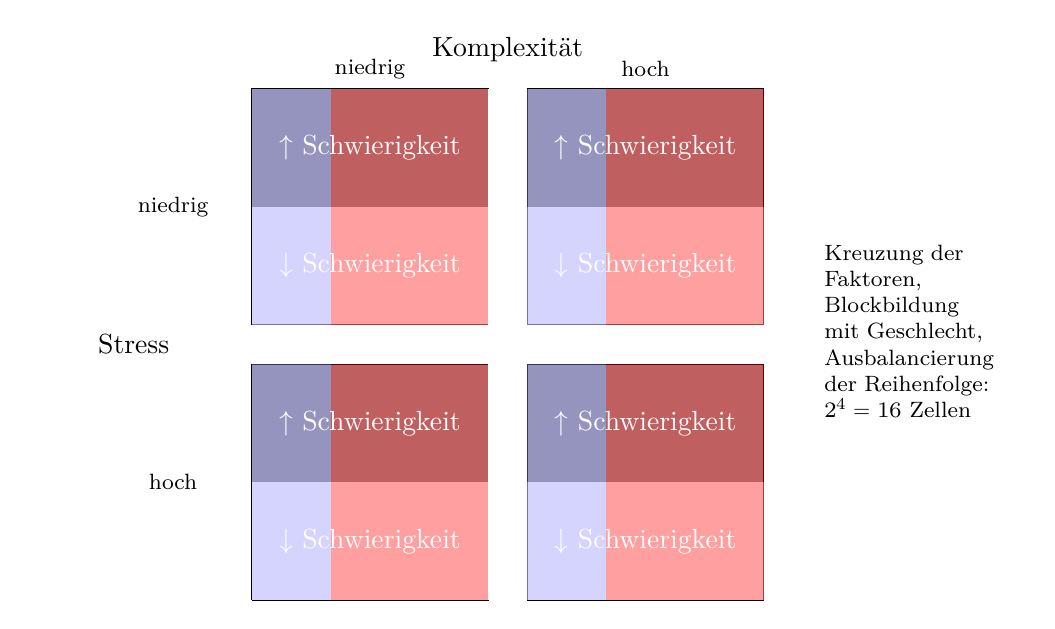
\begin{tikzpicture}
\tikzset{
    mytext/.style={text width=7em,align=center},
    mylabel/.style={text width=7em,align=center, font=\footnotesize}
}

  \draw (1,1) -- (4,1) -- (4,4) -- (1,4) -- (1,1);
  \draw (4.5,4.5) -- (7.5,4.5) -- (7.5,7.5) -- (4.5,7.5) -- (4.5,4.5);
  \draw (1,4.5) -- (4,4.5) -- (4,7.5) -- (1,7.5) -- (1,4.5);
  \draw (4.5,1) -- (4.5,4) -- (7.5,4) -- (7.5,1) -- (4.5,1);
  \fill [Red, opacity=.5] (2,1) rectangle (4,7.5);
  \fill [Red, opacity=.5] (5.5,1) rectangle (7.5,7.5);
  \fill [Blue, opacity=.5] (1,1) rectangle (2,7.5);
  \fill [Blue, opacity=.5] (4.5,1) rectangle (5.5,7.5);
  
  
  \fill [White, opacity=.25] (1,1) rectangle (7.5,2.5);
  \fill [White, opacity=.25] (1,4.5) rectangle (7.5,6);
  \fill [Black, opacity=.25] (1,2.5) rectangle (7.5,4);
  \fill [Black, opacity=.25] (1,6) rectangle (7.5,7.5);
  

  \fill [White, opacity=1] (1,4) rectangle (7.5,4.5);
  \fill [White, opacity=1] (4,1) rectangle (4.5,7.5);
  
  \node[mytext] at (2.5,3.25) {\textcolor{White}{$\uparrow$ Schwierigkeit}};
  \node[mytext] at (2.5,1.75) {\textcolor{White}{$\downarrow$ Schwierigkeit}};
    \node[mytext] at (2.5,6.75) {\textcolor{White}{$\uparrow$ Schwierigkeit}};
  \node[mytext] at (2.5,5.25) {\textcolor{White}{$\downarrow$ Schwierigkeit}};
    \node[mytext] at (6,3.25) {\textcolor{White}{$\uparrow$ Schwierigkeit}};
  \node[mytext] at (6,1.75) {\textcolor{White}{$\downarrow$ Schwierigkeit}};
    \node[mytext] at (6,6.75) {\textcolor{White}{$\uparrow$ Schwierigkeit}};
  \node[mytext] at (6,5.25) {\textcolor{White}{$\downarrow$ Schwierigkeit}};
  
    \node[mylabel] at (2.5,7.75) {niedrig};
  \node[mylabel] at (6,7.75) {hoch};
  \node[mylabel] at (0,6) {niedrig};
  \node[mylabel] at (0,2.5) {hoch};
  \node[mytext] at (-0.5,4.25) {Stress};
  \node[mytext] at (4.25,8) {Komplexität};
  \node[mylabel] at(9.5, 4.25) {Kreuzung der \newline Faktoren, \newline Blockbildung \newline mit Geschlecht, \newline Ausbalancierung \newline der Reihenfolge: \newline $2^4=16$ Zellen \newline};
\end{tikzpicture}

\hypertarget{experimentelle-vs.-nicht-experimentelle-studien}{%
\subsection{experimentelle vs.~nicht-experimentelle Studien}\label{experimentelle-vs.-nicht-experimentelle-studien}}

\begin{tabular}[t]{ll}
\toprule
Nicht-experimentelle Studien &  Experimentelle Studien\\
\midrule
Vermutete Ursachen nur gemessen & Ursachen werden erzeugt\\
Zeitliche Reihenfolge oft unklar & Ursache kommt vor Wirkung\\
Störvariablen nur messbar (\$\textbackslash{}neq\$ Kontrolle) & Gute Kontrolle von Störvariablen\\
unbekannte Störvariablen nie kontrollierbar & z.T. auch unbekannte Störvariablen kontrollierbar\\
Kausalschluss nicht möglich & Kausalschluss möglich\\
\addlinespace
Meist möglich & Nicht immer möglich (praktisch, ethisch)\\
Eher natürliches Setting & Eher künstliches Setting\\
\bottomrule
\end{tabular}

\hypertarget{gruppenarbeit}{%
\subsection{Gruppenarbeit}\label{gruppenarbeit}}

Gibt's im \href{https://lms.uni-kiel.de/auth/RepositoryEntry/3715989588/CourseNode/102596614637734}{Olat}.

\hypertarget{personen-im-experiment}{%
\subsection{Personen im Experiment}\label{personen-im-experiment}}

\hypertarget{versuchsleiter-vl}{%
\subsubsection{Versuchsleiter (VL)}\label{versuchsleiter-vl}}

\begin{itemize}
\tightlist
\item
  Synonym: Experimentator (experimenter)
\end{itemize}

\hypertarget{versuchsperson}{%
\subsubsection{Versuchsperson}\label{versuchsperson}}

\begin{itemize}
\item
  Synonyme: Proband (subject), Teilnehmer (participant)
\item
  Manchmal auch Versuchstiere (subject, test animal)
\end{itemize}

\hypertarget{variablen-im-experiment}{%
\subsection{Variablen im Experiment}\label{variablen-im-experiment}}

\hypertarget{unabhuxe4ngige-variable-uv}{%
\subsubsection{unabhängige Variable (UV)}\label{unabhuxe4ngige-variable-uv}}

\begin{itemize}
\tightlist
\item
  Synonyme: independent variable, Behandlung (treatment), Faktor (factor), Bedingung (condition)
\item
  \(\rightarrow\) Variable, die vom Experimentator aktiv verändert, variiert, manipuliert wird
\end{itemize}

\hypertarget{abhuxe4ngige-variable-av}{%
\subsubsection{abhängige Variable (AV)}\label{abhuxe4ngige-variable-av}}

\begin{itemize}
\tightlist
\item
  Synonyme: dependent Variable, primary and secondary outcome
\item
  \(\rightarrow\) Variable, bei der der Effekt der UV beobachtet werden soll
\end{itemize}

\hypertarget{stuxf6rvariable}{%
\subsubsection{Störvariable}\label{stuxf6rvariable}}

\begin{itemize}
\tightlist
\item
  Synonyme: extraneous variable, confounding variable
\item
  \(\rightarrow\) Variable, die (vermutlich) ebenfalls die AV beeinflusst, deren Wirkung im Experiment neutralisiert (=kontrolliert) werden soll, weil sie den Effekt der UV stören würde.
\item
  Keine Kontrolle \(\rightarrow\) Konfundierung von UV und Störvariable

  \begin{itemize}
  \tightlist
  \item
    Mediatorvariable

    \begin{itemize}
    \tightlist
    \item
      mediiert (vermittelt als Zwischenglied die Wirkung von UV auf AV
    \item
      \(\rightarrow\) Ohne Mediator keine Wirkung von UV auf AV
    \end{itemize}
  \item
    Moderatorvariable

    \begin{itemize}
    \tightlist
    \item
      moderiert (verändert) die Art der Wirkung von UV auf AV
    \item
      \(\rightarrow\) Unterschiedliche Wirkung der UV je nach Ausprägung des Moderators
    \end{itemize}
  \end{itemize}
\end{itemize}

\hypertarget{typen-von-studien-experimenten}{%
\section{Typen von Studien / Experimenten}\label{typen-von-studien-experimenten}}

\hypertarget{typen-von-studien}{%
\subsection{Typen von Studien}\label{typen-von-studien}}

\hypertarget{experimente}{%
\subsubsection{Experimente}\label{experimente}}

\begin{itemize}
\tightlist
\item
  UV kann wirklich manipuliert werden, SV können kontrolliert werden
\item
  z.B. UV: Verum vs.~Placebo, AV: Depressivität, SV: randomisiert, doppelblind, Crossover
\end{itemize}

\hypertarget{quasiexperimente}{%
\subsubsection{Quasiexperimente}\label{quasiexperimente}}

\begin{itemize}
\tightlist
\item
  Störvariablen können nicht richtig kontrolliert werden
\item
  z.B. Vergleich verschiedener Lehrmethoden mit gegebenen Schulklassen
\end{itemize}

\hypertarget{ex-post-facto-studie}{%
\subsubsection{Ex-Post-Facto-Studie}\label{ex-post-facto-studie}}

\begin{itemize}
\tightlist
\item
  UV kann nicht manipuliert, sondern nur gemessen werden
\item
  Z.B. Vergleich von Patienten vs.~Gesunden hinsichtlich Gedächtnisleistung
\end{itemize}

\hypertarget{nichtexperimentelle-studien}{%
\subsubsection{Nichtexperimentelle Studien}\label{nichtexperimentelle-studien}}

\begin{itemize}
\tightlist
\item
  UV wird nicht manipuliert, Störvariablen (so gut wie) gar nicht kontrolliert
\item
  z.B. Längsschnittstudien zur Entwicklung des Gedächtnisses
  z.B. Querschnittstudien zum Zusammenhang von X und Y
\end{itemize}

\hypertarget{kategorisierung-von-studien}{%
\subsection{Kategorisierung von Studien}\label{kategorisierung-von-studien}}

\hypertarget{einteilung-nach-dem-ort}{%
\subsubsection{Einteilung nach dem „Ort``}\label{einteilung-nach-dem-ort}}

\begin{itemize}
\tightlist
\item
  Laborexperiment

  \begin{itemize}
  \tightlist
  \item
    gute Kontrolle von Störvariablen, u.U. schlechte Generalisierbarkeit
  \end{itemize}
\item
  Feldexperiment

  \begin{itemize}
  \tightlist
  \item
    schlechte Kontrolle von Störvariablen, gute Generalisierbarkeit
  \item
    \(\neq\) nichtexperimentelle Feldstudie (z.B. „Anwendungsbeobachtung``)
  \end{itemize}
\end{itemize}

\hypertarget{spezielfall-online-studien}{%
\subsection{Spezielfall: online-Studien}\label{spezielfall-online-studien}}

\hypertarget{vorteile}{%
\subsubsection{Vorteile}\label{vorteile}}

\begin{itemize}
\item
  Großes N mit geringem Aufwand
\item
  Kein Versuchsleiter \(\rightarrow\) Keine Versuchsleitereffekte
\item
  Standardisierung von Instruktionen und Ablauf
\item
  Jederzeit durchführbar
\end{itemize}

\hypertarget{nachteile}{%
\subsubsection{Nachteile}\label{nachteile}}

\begin{itemize}
\tightlist
\item
  Selbstselektion (z.B. Menschen mit genügend Freizeit und Zugang zu Rechner)
\item
  Die Angaben der Vp sind nicht überprüfbar
\item
  Mehrfachteilnahme nicht kontrollierbar
\item
  Keine Standardisierung von Technik, Umgebung, Situation, Störungen \ldots{}
\item
  Schummeln, Vorsagen, soziale Erwünschtheit (z.B. Partner guckt bei Umfrage zu Pornokonsum zu)
\item
  Keine Kontrolle des aktuellen Zustands der Vp (z.B. müde, betrunken, krank, \ldots)
\end{itemize}

\hypertarget{fallbeispiele}{%
\section{Fallbeispiele}\label{fallbeispiele}}

\hypertarget{fragen}{%
\subsection{Fragen:}\label{fragen}}

Texte sind im Olat.

\begin{enumerate}
\def\labelenumi{\arabic{enumi}.}
\tightlist
\item
  Fragestellung: Was sollte untersucht werden?
\item
  Was ist/sind hier die unabhängige/n Variable/n? Welche Stufen hatte/n diese?
\item
  Was ist/sind hier die abhängige/n Variable/n? Wie wurde/n diese gemessen?
\item
  Handelt es sich um eine Labor oder eine Feldstudie?
\item
  Handelt es sich um ein Experiment, Quasiexperiment oder sonstige Studie?
\end{enumerate}

\hypertarget{ausblick-1}{%
\section{Ausblick}\label{ausblick-1}}

\begin{itemize}
\tightlist
\item
  Störvariablen und ihre Kontrolle
\item
  Varianz: Freund und Feind
\item
  Validitäten
\end{itemize}

\hypertarget{anhang}{%
\section{Anhang}\label{anhang}}

\hypertarget{beispiel-elfmeterschieuxdfen}{%
\subsection{Beispiel Elfmeterschießen}\label{beispiel-elfmeterschieuxdfen}}

\hypertarget{fragen-antworten}{%
\subsubsection{Fragen \& Antworten:}\label{fragen-antworten}}

\begin{enumerate}
\def\labelenumi{\arabic{enumi}.}
\tightlist
\item
  Was ist/sind hier die unabhängige/n Variable/n? \smallskip \newline Anlaufwinkel (mit 6 Stufen: 0° bis 50°) \smallskip \newline
\item
  Was ist/sind hier die abhängige/n Variable/n? \smallskip \newline Genauigkeit der Vorhersage der Schussrichtung \smallskip \newline
\item
  Handelt es sich um eine Labor oder eine Feldstudie? \smallskip \newline Labor (Stimuli wurden zwar auf dem Feld erzeugt, Experiment aber im Labor) \smallskip \newline
\item
  Handelt es sich um ein Experiment, Quasiexperiment oder sonstige Studie? \smallskip \newline Echtes Experiment (UV manipuliert, Störvariablen kontrolliert, AV gemessen)
\end{enumerate}

\hypertarget{beispiel-cannabis}{%
\subsection{Beispiel Cannabis}\label{beispiel-cannabis}}

\hypertarget{fragen-antworten-1}{%
\subsubsection{Fragen \& Antworten:}\label{fragen-antworten-1}}

\begin{enumerate}
\def\labelenumi{\arabic{enumi}.}
\tightlist
\item
  Was ist/sind hier die unabhängige/n Variable/n? \smallskip \newline Keine. Cannabiskonsum (ja/nein) ist nicht manipuliert worden, daher quasi-UV \smallskip \newline
\item
  Was ist/sind hier die abhängige/n Variable/n? \smallskip \newline Gedächtnis, Aufmerksamkeit \smallskip \newline
\item
  Handelt es sich um eine Labor- oder eine Feldstudie? \smallskip \newline Laborstudie \smallskip \newline
\item
  Handelt es sich um ein Experiment, Quasiexperiment oder sonstige Studie? \smallskip \newline Quasiexperiment
\end{enumerate}

\hypertarget{beispiel-stressbewuxe4ltigung}{%
\subsection{Beispiel Stressbewältigung}\label{beispiel-stressbewuxe4ltigung}}

\hypertarget{fragen-antworten-2}{%
\subsubsection{Fragen \& Antworten:}\label{fragen-antworten-2}}

\begin{enumerate}
\def\labelenumi{\arabic{enumi}.}
\tightlist
\item
  Was ist/sind hier die unabhängige/n Variable/n? \smallskip \newline Stressbewältigungsprogramm (Ja/nein), Messzeitpunkt (prä/post) \smallskip \newline
\item
  Was ist/sind hier die abhängige/n Variable/n? \smallskip \newline Gesundheitsrelevante Parameter (sehr viele) \smallskip \newline
\item
  Handelt es sich um eine Labor- oder eine Feldstudie? \smallskip \newline Laborstudie \smallskip \newline
\item
  Handelt es sich um ein Experiment, Quasiexperiment oder sonstige Studie? \smallskip \newline Experiment
\end{enumerate}

\hypertarget{beispiel-sport-macht-mich-high}{%
\subsection{Beispiel Sport macht mich high}\label{beispiel-sport-macht-mich-high}}

\hypertarget{fragen-antworten-3}{%
\subsubsection{Fragen \& Antworten:}\label{fragen-antworten-3}}

\begin{enumerate}
\def\labelenumi{\arabic{enumi}.}
\tightlist
\item
  Was ist/sind hier die unabhängige/n Variable/n? \smallskip \newline Messzeitpunkte, Katamnese \smallskip \newline
\item
  Was ist/sind hier die abhängige/n Variable/n? \smallskip \newline nicht gut definiert, Drogenmissbrauch, Körpergefühl, Fitness, Motivation \ldots{} \smallskip \newline
\item
  Handelt es sich um eine Labor- oder eine Feldstudie? \smallskip \newline Laborstudie \smallskip \newline
\item
  Handelt es sich um ein Experiment, Quasiexperiment oder sonstige Studie? \smallskip \newline Sonstige Studie („Anwendungsbeobachtung``)
\end{enumerate}

\hypertarget{literaturrecherche}{%
\chapter{Literaturrecherche}\label{literaturrecherche}}

\hypertarget{organisatorisches-3}{%
\section{Organisatorisches}\label{organisatorisches-3}}

\hypertarget{semesterplan-4}{%
\subsection{Semesterplan}\label{semesterplan-4}}

\begin{tabular}[t]{rll}
\toprule
Sitzung & Datum & Sitzungstitel\\
\midrule
1 & 02.11.2020 & Warum wissenschaftliche Psychologie\\
2 & 28.11.2020
29.11.2020 & Hypothesen und der Prozess der Hypothesenprüfung\\
3 & 28.11.2020
29.11.2020 & Experimentelles Vorgehen\\
4 & 28.11.2020
29.11.2020 & Literaturrecherche\\
5 & 28.11.2020
29.11.2020 & Operationalisieren und Messen\\
\addlinespace
6 & 12.12.2020
13.12.2020 & Experimentelle Versuchspläne\\
7 & 12.12.2020
13.12.2020 & Störvariablen im Experiment\\
8 & 12.12.2020
13.12.2020 & Nicht-experimentelle Versuchspläne\\
9 & 12.12.2020
13.12.2020 & Material und Stichprobe\\
10 & 23.1.2021
24.1.2021 & Auswertung, Darstellung und Interpretation\\
\addlinespace
11 & 23.1.2021
24.1.2021 & Ethische Probleme im Versuch\\
12 & 23.1.2021
24.1.2021 & Publikationsprozess\\
13 & wird noch bekannt gegeben & Vorstellung der Gruppenarbeiten\\
14 & wird noch bekannt gegeben & Klausurvorbereitung\\
\bottomrule
\end{tabular}

\hypertarget{wiederholung-2}{%
\section{Wiederholung}\label{wiederholung-2}}

\hypertarget{kausalschluxfcsse}{%
\subsection{Kausalschlüsse}\label{kausalschluxfcsse}}

\begin{cols}

\begin{col}{0.50\textwidth}

\begin{center}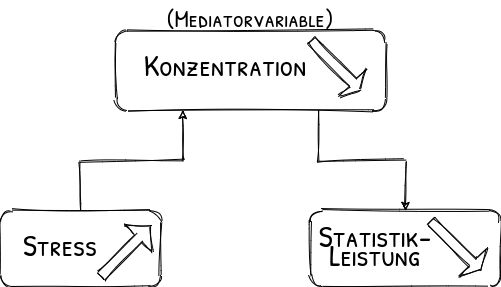
\includegraphics[width=150pt]{imgs/mediator_causality} \end{center}

\begin{center}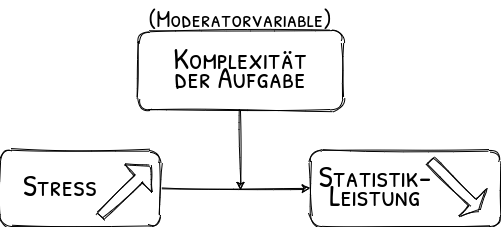
\includegraphics[width=150pt]{imgs/moderator_causality} \end{center}

\end{col}

\begin{col}{0.5\textwidth}

\begin{center}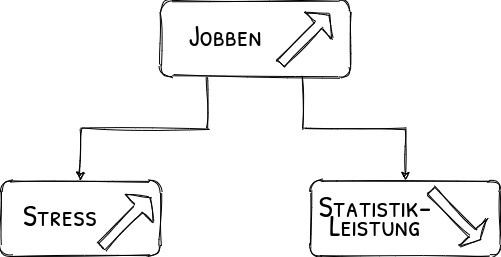
\includegraphics[width=150pt]{imgs/confound_causality} \end{center}

\end{col}

\end{cols}

\hypertarget{design-1}{%
\subsection{Design:}\label{design-1}}

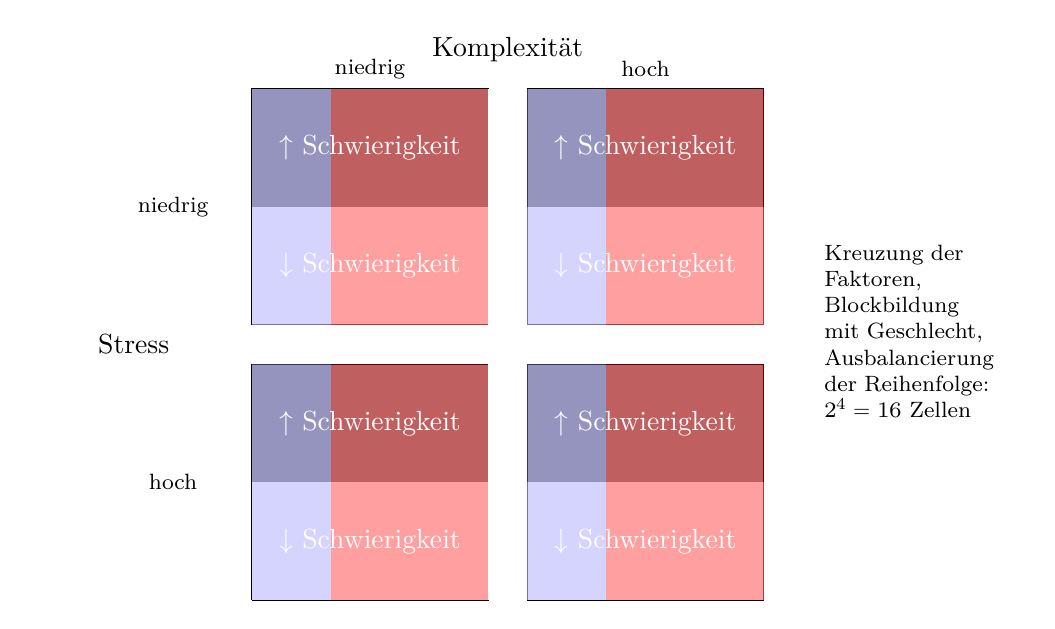
\begin{tikzpicture}
\tikzset{
    mytext/.style={text width=7em,align=center},
    mylabel/.style={text width=7em,align=center, font=\footnotesize}
}

  \draw (1,1) -- (4,1) -- (4,4) -- (1,4) -- (1,1);
  \draw (4.5,4.5) -- (7.5,4.5) -- (7.5,7.5) -- (4.5,7.5) -- (4.5,4.5);
  \draw (1,4.5) -- (4,4.5) -- (4,7.5) -- (1,7.5) -- (1,4.5);
  \draw (4.5,1) -- (4.5,4) -- (7.5,4) -- (7.5,1) -- (4.5,1);
  \fill [Red, opacity=.5] (2,1) rectangle (4,7.5);
  \fill [Red, opacity=.5] (5.5,1) rectangle (7.5,7.5);
  \fill [Blue, opacity=.5] (1,1) rectangle (2,7.5);
  \fill [Blue, opacity=.5] (4.5,1) rectangle (5.5,7.5);
  
  
  \fill [White, opacity=.25] (1,1) rectangle (7.5,2.5);
  \fill [White, opacity=.25] (1,4.5) rectangle (7.5,6);
  \fill [Black, opacity=.25] (1,2.5) rectangle (7.5,4);
  \fill [Black, opacity=.25] (1,6) rectangle (7.5,7.5);
  

  \fill [White, opacity=1] (1,4) rectangle (7.5,4.5);
  \fill [White, opacity=1] (4,1) rectangle (4.5,7.5);
  
  \node[mytext] at (2.5,3.25) {\textcolor{White}{$\uparrow$ Schwierigkeit}};
  \node[mytext] at (2.5,1.75) {\textcolor{White}{$\downarrow$ Schwierigkeit}};
    \node[mytext] at (2.5,6.75) {\textcolor{White}{$\uparrow$ Schwierigkeit}};
  \node[mytext] at (2.5,5.25) {\textcolor{White}{$\downarrow$ Schwierigkeit}};
    \node[mytext] at (6,3.25) {\textcolor{White}{$\uparrow$ Schwierigkeit}};
  \node[mytext] at (6,1.75) {\textcolor{White}{$\downarrow$ Schwierigkeit}};
    \node[mytext] at (6,6.75) {\textcolor{White}{$\uparrow$ Schwierigkeit}};
  \node[mytext] at (6,5.25) {\textcolor{White}{$\downarrow$ Schwierigkeit}};
  
    \node[mylabel] at (2.5,7.75) {niedrig};
  \node[mylabel] at (6,7.75) {hoch};
  \node[mylabel] at (0,6) {niedrig};
  \node[mylabel] at (0,2.5) {hoch};
  \node[mytext] at (-0.5,4.25) {Stress};
  \node[mytext] at (4.25,8) {Komplexität};
  \node[mylabel] at(9.5, 4.25) {Kreuzung der \newline Faktoren, \newline Blockbildung \newline mit Geschlecht, \newline Ausbalancierung \newline der Reihenfolge: \newline $2^4=16$ Zellen \newline};
\end{tikzpicture}

\hypertarget{experimentelle-vs.-nicht-experimentelle-studien-1}{%
\subsection{experimentelle vs.~nicht-experimentelle Studien}\label{experimentelle-vs.-nicht-experimentelle-studien-1}}

\begin{tabular}[t]{ll}
\toprule
Nicht-experimentelle Studien &  Experimentelle Studien\\
\midrule
Vermutete Ursachen nur gemessen & Ursachen werden erzeugt\\
Zeitliche Reihenfolge oft unklar & Ursache kommt vor Wirkung\\
Störvariablen nur messbar (\$\textbackslash{}neq\$ Kontrolle) & Gute Kontrolle von Störvariablen\\
unbekannte Störvariablen nie kontrollierbar & z.T. auch unbekannte Störvariablen kontrollierbar\\
Kausalschluss nicht möglich & Kausalschluss möglich\\
\addlinespace
Meist möglich & Nicht immer möglich (praktisch, ethisch)\\
Eher natürliches Setting & Eher künstliches Setting\\
\bottomrule
\end{tabular}

\hypertarget{literaturrecherche-1}{%
\section{Literaturrecherche}\label{literaturrecherche-1}}

\hypertarget{wozu-uxfcberhaupt}{%
\subsection{Wozu überhaupt?}\label{wozu-uxfcberhaupt}}

\begin{cols}

\begin{col}{0.30\textwidth}

\begin{center}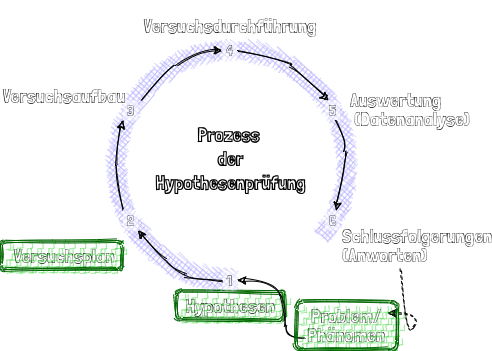
\includegraphics[width=150pt]{imgs/hypothesen_lit} \end{center}

\end{col}

\begin{col}{0.68\textwidth}

\textbf{Theorie:}

Überblick über bisherige Forschung verschaffen um:

\begin{enumerate}
\def\labelenumi{\alph{enumi})}
\item
  Ein beobachtetes Phänomen in bestehende Theorien einzuordnen
\item
  Hypothesen über ein Phänomen abzuleiten
\item
  Nachzulesen welche Umsetzungsparameter für meine Studie vielversprechend sind
\end{enumerate}

\end{col}

\end{cols}

\hypertarget{wo}{%
\subsection{Wo?}\label{wo}}

\hypertarget{psychinfo}{%
\subsubsection{PsychINFO}\label{psychinfo}}

\begin{itemize}
\tightlist
\item
  Internationale bibliographische Datenbank
\item
  Schwerpunkt: Psychologie / Sonstige: verwandte Gebiete wie Psychiatrie, Soziologie, Erziehungswissenschaften, Anthropologie, Pharmakologie, Physiologie, Kriminologie und Linguistik
\item
  Zeitschriftenaufsätze, Bücher, Buchkapitel, Buchbesprechungen, Forschungsberichte, Fallstudien
\item
  Von der APA gepflegt
\end{itemize}

\hypertarget{psyndex-tests}{%
\subsubsection{PSYNDEX Tests}\label{psyndex-tests}}

\begin{itemize}
\tightlist
\item
  Deutschsprachige Datenbank
\item
  Schwerpunkt: psychologischen Testverfahren
\item
  Rezensionen von Skalen, Fragebögen, Leistungstest
\end{itemize}

\hypertarget{pubmed}{%
\subsubsection{Pubmed}\label{pubmed}}

\begin{itemize}
\tightlist
\item
  Internationale bibliographische Datenbank
\item
  Schwerpunkt: Medizin / Sonstige: Medizin, Biologie, Psychologie etc.
\item
  Biomedizinische Zeitschriften und online-Bücher
\item
  Volltext oder Links zu Volltext
\end{itemize}

\hypertarget{google-scholar}{%
\subsubsection{Google Scholar}\label{google-scholar}}

\begin{itemize}
\tightlist
\item
  Internationale bibliographische Suchmaschine
\item
  Schwerpunkt: gibt es nicht
\item
  Zeitschriftenaufsätze, Bücher, Buchkapitel, Buchbesprechungen, Forschungsberichte, Fallstudien,\ldots{}
\item
  teilweise Links zu Volltexten, oft nur Titelübersicht
\end{itemize}

\hypertarget{web-of-science}{%
\subsubsection{Web of Science}\label{web-of-science}}

\begin{itemize}
\tightlist
\item
  Internationale (vorwiegend englischsprachige) Datenbank
\item
  Schwerpunkt: Liste von redaktionell ausgewählten Journals
\item
  vorwiegend Zeitschriftenaufsätze
\item
  teilweise Links zu Volltexten aus dem Uninetz
\end{itemize}

\hypertarget{testzentrale}{%
\subsubsection{Testzentrale}\label{testzentrale}}

\begin{itemize}
\tightlist
\item
  (kommerzielle) Website vom Hogrefe-Verlag
\item
  Schwerpunkt: Verkauf von Hogrefe-Testverfahren
\item
  Aber in der Übersicht zu den Tests Rezensionen von Skalen, Fragebögen, Leistungstest
\end{itemize}

\hypertarget{links}{%
\subsection{Links}\label{links}}

\href{http://rzblx10.uni-regensburg.de/dbinfo/dbliste.php?bib_id=ubk\&colors=15\&ocolors=40\&lett=f\&gebiete=22}{PsychINFO und PSYNDEX} (Nur aus dem Uninetz nutzbar)

\href{https://www.ncbi.nlm.nih.gov/pubmed}{Pubmed}

\href{https://scholar.google.de/}{Google Scholar}

\href{https://apps.webofknowledge.com/WOS_GeneralSearch_input.do?product=WOS\&search_mode=GeneralSearch\&SID=C2nuroLClfkbQeKY4ub\&preferencesSaved=}{Web of Science}

\href{https://www.testzentrale.de/}{Testzentrale}

\hypertarget{wie-studien-finden}{%
\subsection{Wie Studien finden?}\label{wie-studien-finden}}

\begin{itemize}
\item
  Schneeballsystem

  \begin{itemize}
  \tightlist
  \item
    mit Übersichtsarbeiten anfangen (Reviews, Metaanalysen, Lehrbuchkapitel,\ldots)
  \item
    an Literaturhinweisen `entlang hangeln'
  \end{itemize}
\item
  Autorenorientiertes Vorgehen

  \begin{itemize}
  \tightlist
  \item
    anhand von allgemeinen Suchbegriffen Arbeitsgruppe(n) finden
  \item
    anhand der Autoren nach anderen Studien suchen
  \end{itemize}
\end{itemize}

\hypertarget{wie-studien-beschaffen}{%
\subsection{Wie Studien beschaffen?}\label{wie-studien-beschaffen}}

\begin{itemize}
\tightlist
\item
  PDF-link in pubmed folgen (nur im Netz der Uni)
\item
  Google: „Titel" filetype:pdf
\item
  Von den Betreuenden
\item
  Über ResearchGate/Mendeley geteilte Artikel downloaden
\item
  Communicating author anschreiben und um PDF bitten
\item
  Fernleihe
\item
  Gebührenpflichtige Direktlieferdienste (Subito)
\item
  \ldots{}
\end{itemize}

\hypertarget{was-mache-ich-mit-den-beschafften-studien}{%
\subsection{Was mache ich mit den beschafften Studien?}\label{was-mache-ich-mit-den-beschafften-studien}}

\hypertarget{verwalten}{%
\subsubsection{verwalten}\label{verwalten}}

\begin{itemize}
\item
  Citavi (Windows \& Mac)

  \begin{itemize}
  \tightlist
  \item
    vom RZ gestellt: \href{https://www.rz.uni-kiel.de/de/angebote/software/citavi}{Citavi beim RZ}
  \end{itemize}
\item
  Endnote (Windows)
\item
  Mendeley (Windows, Linux \& Mac)

  \begin{itemize}
  \tightlist
  \item
    kostenlos, gehört aber zu Elsvier
  \end{itemize}
\item
  Zotero (Windows, Linux \& Mac)

  \begin{itemize}
  \tightlist
  \item
    Open Source, \href{https://www.zotero.org/}{hier} erhältlich
  \end{itemize}
\end{itemize}

\hypertarget{richtig-zitieren}{%
\subsubsection{Richtig zitieren}\label{richtig-zitieren}}

\begin{itemize}
\item
  \href{https://elibrary.hogrefe.de/book/99.110005/9783840927638}{formale Richtlinien laut DGPs}
\item
  \href{https://en.wikipedia.org/wiki/APA_style}{wikipedia-Seite mit Zitationsbeispielen nach APA Style 6}
\end{itemize}

\hypertarget{rechercheaufgaben-pubmed}{%
\subsection{Rechercheaufgaben Pubmed}\label{rechercheaufgaben-pubmed}}

\begin{enumerate}
\def\labelenumi{\arabic{enumi}.}
\item
  Neuere Übersichtsartikel zu einem Thema finden

  \begin{itemize}
  \tightlist
  \item
    Sie möchten wissen, ob Sport („Exercise``) bei Depression („depression'') hilft. Finden Sie einen Übersichtsartikel („Review"), der den aktuellen Forschungsstand zusammenfasst. \smallskip
  \end{itemize}
\item
  Einen bestimmten Artikel finden

  \begin{itemize}
  \tightlist
  \item
    Ihr Bachelorarbeitsbetreuer erinnert sich dunkel, dass mal in der Zeitschrift „Science" ein Artikel mit dem Titel „By Carrot or by Stick" erschienen ist. Finden Sie die Literaturangabe, besorgen sie den Artikel und finden Sie die Homepage des Erstautors. \smallskip
  \end{itemize}
\item
  Artikeln eines Autors finden

  \begin{itemize}
  \tightlist
  \item
    Von einer Kommilitonin haben Sie den Tipp bekommen, dass der Autor Jan Born interessante Artikel zum Thema Schlaf geschrieben hat. Finden Sie einen neueren Artikel von Born zum Thema Gedächtniskonsolidierung („consolidation``) im Schlaf („sleep'').
  \end{itemize}
\end{enumerate}

\hypertarget{rechercheaufgaben-psyndex-tests}{%
\subsection{Rechercheaufgaben PsynDex Tests:}\label{rechercheaufgaben-psyndex-tests}}

\begin{enumerate}
\def\labelenumi{\arabic{enumi}.}
\item
  Skalen zur Sozialen Angststoerung (SOZAS)

  \begin{itemize}
  \tightlist
  \item
    Finden Sie heraus für welche Altersgruppe die SOZAS geeignet sind.
  \item
    Wo kann man das Instrument kaufen und wieviel kostet es?
  \end{itemize}
\end{enumerate}

\begin{enumerate}
\def\labelenumi{\arabic{enumi}.}
\setcounter{enumi}{1}
\item
  Selbstwert

  \begin{itemize}
  \tightlist
  \item
    Finden Sie ein Instrument, mit dem man Selbstwert bei Kindern messen kann.
  \end{itemize}
\item
  Procrastination

  \begin{itemize}
  \tightlist
  \item
    Finden Sie einen Fragebogen, mit dem man Procrastination (Aufschieberitis) bei Jugendlichen und Erwachsenen messen kann.
  \end{itemize}
\end{enumerate}

\hypertarget{rechercheaufgabe-web-of-science}{%
\subsection{Rechercheaufgabe Web of Science:}\label{rechercheaufgabe-web-of-science}}

\begin{enumerate}
\def\labelenumi{\arabic{enumi}.}
\tightlist
\item
  Schneeballsuche
\end{enumerate}

\begin{itemize}
\tightlist
\item
  Sie haben von Ihrem Betreuer mitgeteilt bekommen, dass die Studie ``Job burnout'' von Maslach und anderen aus dem Jahre 2001 eine einflussreiche Arbeit im Bereich der Burnout-Forschung ist. Nun wollen Sie sich einen Überblick darüber verschaffen, wie sich die Zitationen dieses Reviews im zeitlichen Verlauf geändert haben. Erstellen Sie einen entsprechenden Zitationsreport.
\end{itemize}

\begin{enumerate}
\def\labelenumi{\arabic{enumi}.}
\setcounter{enumi}{1}
\tightlist
\item
  Relevante Journals
\end{enumerate}

\begin{itemize}
\tightlist
\item
  Sie haben in vielen Artikeln die folgende Zitation gesehen: ``Faul, F., Erdfelder, E., Lang, A. G., \& Buchner, A. (2007). G* Power 3: A flexible statistical power analysis program for the social, behavioral, and biomedical sciences. Behavior research methods, 39(2), 175-191.'' Da Sie der Einsatz von Power-Berechnungen brennend interessiert, wollen Sie sich einen Überblick über Journals verschaffen, in denen dieser Aufsatz zitiert wurde. Finden Sie die zehn Jounals, in denen das Buch von Cohen am häufigsten zitiert wurde.
\end{itemize}

\hypertarget{hausaufgabe}{%
\subsection{Hausaufgabe}\label{hausaufgabe}}

\hypertarget{vorarbeit-fuxfcr-die-pruxe4sentation}{%
\subsubsection{Vorarbeit für die Präsentation:}\label{vorarbeit-fuxfcr-die-pruxe4sentation}}

\begin{itemize}
\item
  Theoretischen Rahmen ausarbeiten

  \begin{itemize}
  \tightlist
  \item
    Hypothesen dem theoretischen Rahmen anpassen
  \end{itemize}
\item
  Literaturangaben für dafür zu Rate gezogene Studien erstellen (APA/IfP)
\end{itemize}

\hypertarget{operationalisieren-und-messen}{%
\chapter{Operationalisieren und Messen}\label{operationalisieren-und-messen}}

\hypertarget{organisatorisches-4}{%
\section{Organisatorisches}\label{organisatorisches-4}}

\hypertarget{semesterplan-5}{%
\subsection{Semesterplan}\label{semesterplan-5}}

\begin{tabular}[t]{rll}
\toprule
Sitzung & Datum & Sitzungstitel\\
\midrule
1 & 02.11.2020 & Warum wissenschaftliche Psychologie\\
2 & 28.11.2020
29.11.2020 & Hypothesen und der Prozess der Hypothesenprüfung\\
3 & 28.11.2020
29.11.2020 & Experimentelles Vorgehen\\
4 & 28.11.2020
29.11.2020 & Literaturrecherche\\
5 & 28.11.2020
29.11.2020 & Operationalisieren und Messen\\
\addlinespace
6 & 12.12.2020
13.12.2020 & Experimentelle Versuchspläne\\
7 & 12.12.2020
13.12.2020 & Störvariablen im Experiment\\
8 & 12.12.2020
13.12.2020 & Nicht-experimentelle Versuchspläne\\
9 & 12.12.2020
13.12.2020 & Material und Stichprobe\\
10 & 23.1.2021
24.1.2021 & Auswertung, Darstellung und Interpretation\\
\addlinespace
11 & 23.1.2021
24.1.2021 & Ethische Probleme im Versuch\\
12 & 23.1.2021
24.1.2021 & Publikationsprozess\\
13 & wird noch bekannt gegeben & Vorstellung der Gruppenarbeiten\\
14 & wird noch bekannt gegeben & Klausurvorbereitung\\
\bottomrule
\end{tabular}

\hypertarget{wiederholung-3}{%
\section{Wiederholung}\label{wiederholung-3}}

\hypertarget{wozu-uxfcberhaupt-1}{%
\subsection{Wozu überhaupt?}\label{wozu-uxfcberhaupt-1}}

\begin{cols}

\begin{col}{0.30\textwidth}

\begin{center}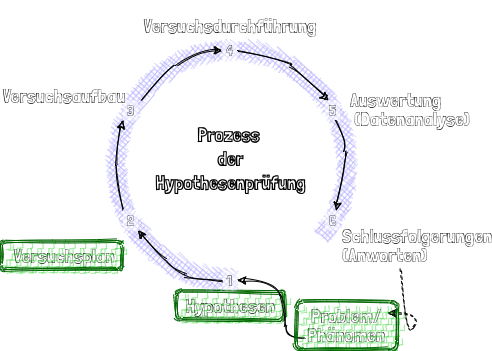
\includegraphics[width=150pt]{imgs/hypothesen_lit} \end{center}

\end{col}

\begin{col}{0.68\textwidth}

\textbf{Theorie:}

Überblick über bisherige Forschung verschaffen um:

\begin{enumerate}
\def\labelenumi{\alph{enumi})}
\item
  Ein beobachtetes Phänomen in bestehende Theorien einzuordnen
\item
  Hypothesen über ein Phänomen abzuleiten
\item
  Nachzulesen welche Umsetzungsparameter für meine Studie vielversprechend sind
\end{enumerate}

\end{col}

\end{cols}

\hypertarget{operationalisierung}{%
\section{Operationalisierung}\label{operationalisierung}}

\hypertarget{operationalisierung-1}{%
\subsection{Operationalisierung:}\label{operationalisierung-1}}

\hypertarget{theoretische-konstrukte-in-beobachtbare-gruxf6uxdfe-uxfcberfuxfchren}{%
\subsubsection{Theoretische Konstrukte in beobachtbare Größe überführen}\label{theoretische-konstrukte-in-beobachtbare-gruxf6uxdfe-uxfcberfuxfchren}}

Beispiel: Welchen Einfluss hat Ängstlichkeit auf Lernen?

\begin{center}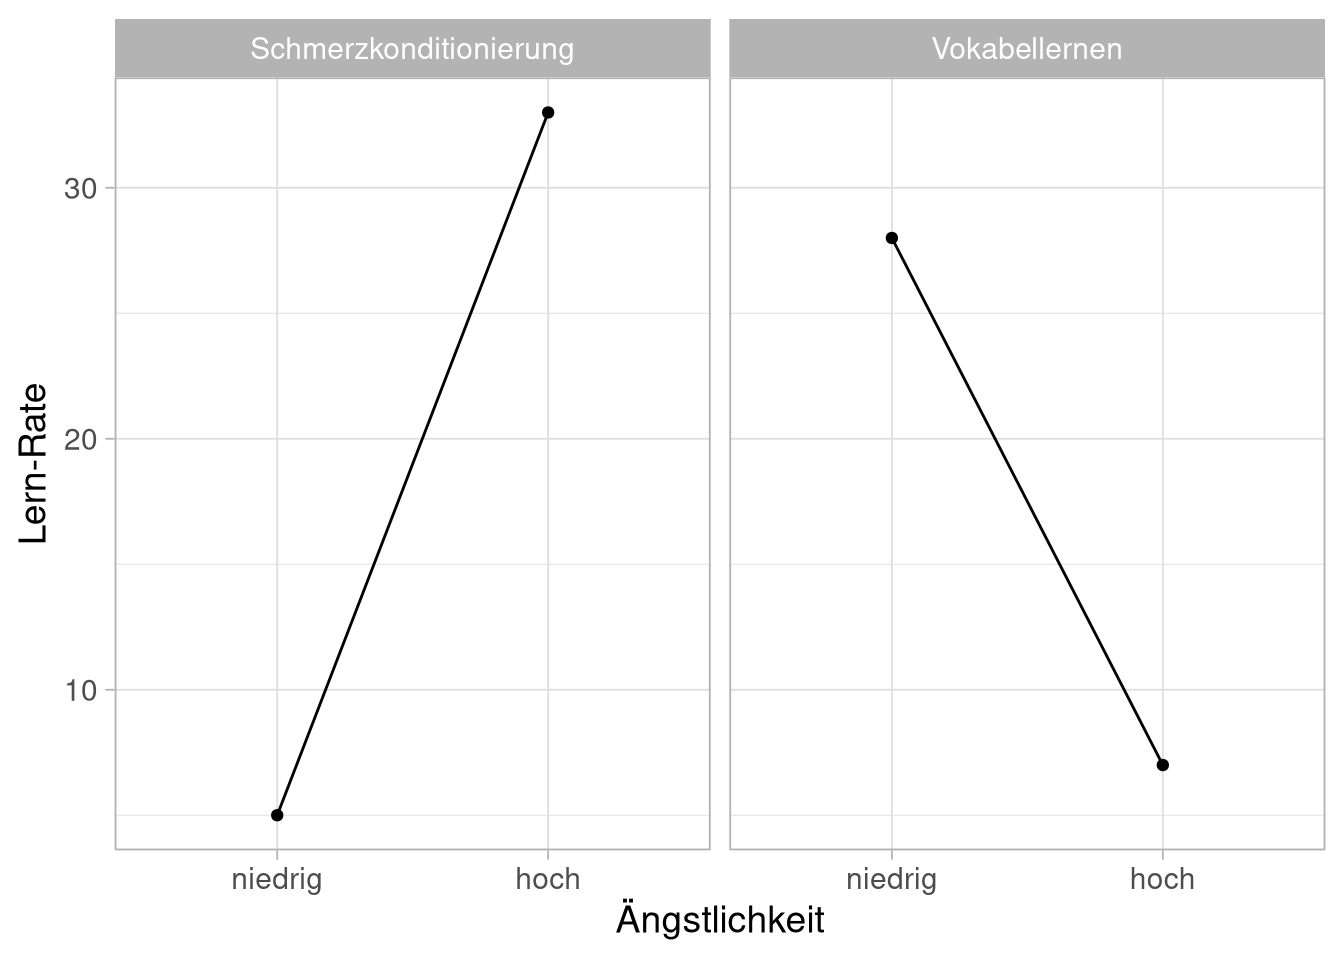
\includegraphics[width=200pt]{Versuchsplanung_WS20_files/figure-latex/lernen_again-1} \end{center}

Hier unterscheidet sich die Operationalisierung der abhängigen Variable (Lernen).
Die widersprüchlichen Ergebnisse zeigen, dass das Konstrukt Lernen nicht einheitlich ist und
die Operationalisierungen verschiedene Aspekte dieses Konstruktes repräsentieren.

\textbf{Operationalisierung} = Definition der genauen Operationen (Handlungen), durch
welche ein theoretisches Konstrukt durch Beobachtung, Zählung, Messung, etc.
erfasst werden soll. Praktische Umsetzung des theoretischen Konstruktes

Ein \textbf{theoretisches \emph{Konstrukt}} ist eine \textbf{nicht direkt beobachtbare komplexe Variable},
welche erst über \textbf{beobachtbare \emph{Indikatoren operationalisiert}} und messbar gemacht
werden muss.

\textbf{Notwendigkeit theoretischer Vorarbeit:} Das theoretische Konstrukt muss zunächst
\textbf{inhaltlich eindeutig definiert} werden, um mögliche Indikatoren zu identifizieren und
zu begründen, welche dann stellvertretend für das theoretische Konstrukt gemessen
werden können.

\begin{center}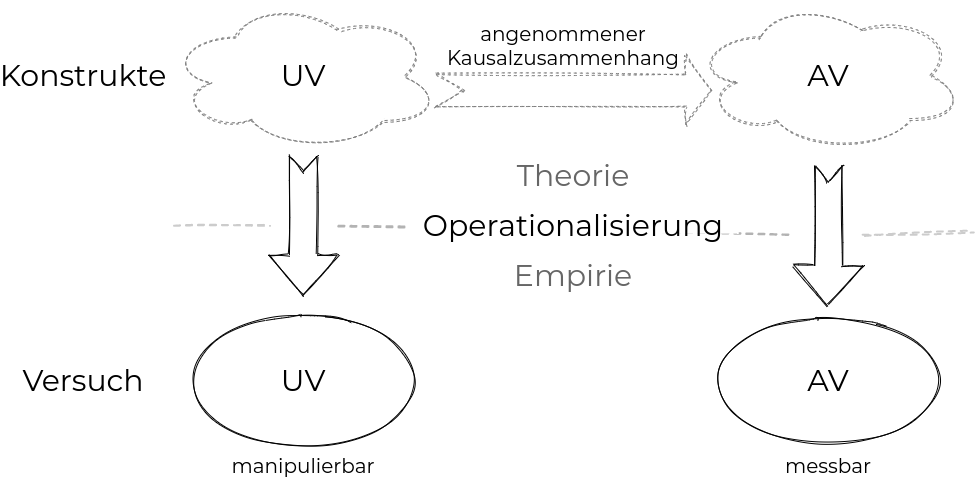
\includegraphics[width=200pt]{imgs/operartionalisierung} \end{center}

\begin{center}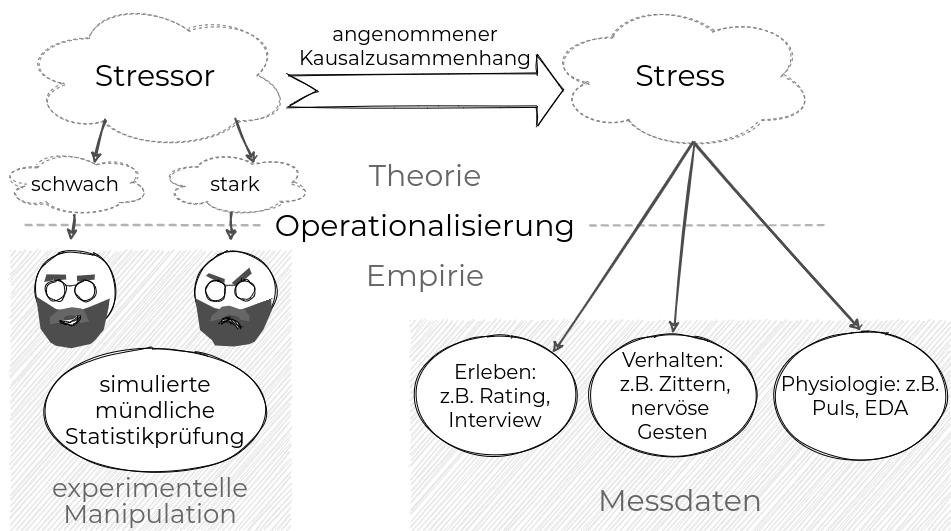
\includegraphics[width=200pt]{imgs/operartionalisierung_stress} \end{center}

\hypertarget{ein-beispiel-wie-entsteht-liebe}{%
\subsubsection{Ein Beispiel: Wie entsteht Liebe?}\label{ein-beispiel-wie-entsteht-liebe}}

\textbf{Hypothese:} Selbstöffnung führt zu interpersonaler Attraktion
(„Wenn man mit dem anderen über persönliche Dinge redet, verliebt man sich.``)

Was ist die unabhängige Variable?

Was ist die abhängige Variable?

Was sind wichtige Störvariablen?

Wie stellen wir die Ausprägungen dieser Variablen her (UV)?

Wie überführen wir diese Variablen (AV) in messbare Größen?

Wie kontrollieren/messen wir diese Variablen (SV)?

Beispiele bei \citet{aronExperimentalGenerationInterpersonal1997} und \citet{sprecherEffectsSelfdisclosureRole2013}

\hypertarget{uv-im-beispiel}{%
\subsubsection{UV im Beispiel:}\label{uv-im-beispiel}}

\begin{cols}

\begin{col}{0.30\textwidth}

\begin{center}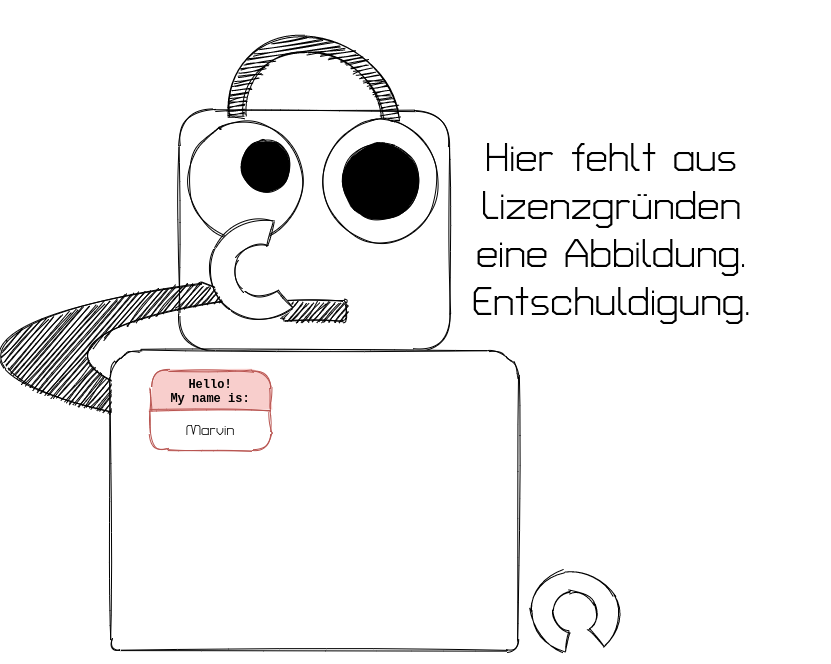
\includegraphics[width=150pt]{imgs/copyright} \end{center}

\end{col}

\begin{col}{0.68\textwidth}

\begin{tabular}[t]{rl}
\toprule
Frage &  \\
\midrule
1 & Given the choice of anyone in the world, whom would you want as a dinner guest?\\
4 & What would you constitute a 'perfect' day for you?\\
7 & Do you have a secret hunch about how you will die?\\
16 & What do you value most in a friendship?\\
17 & What is your most treasured memory?\\
\addlinespace
18 & What does friendship mean to you?\\
20 & What, if anything, is too serious to be joked about?\\
32 & Of all the people in your family, whose death woul you find most disturbing? Why?\\
\bottomrule
\end{tabular}

\href{http://www.focus.de/reisen/zeit-fuer-uns/liebe-als-experiment-die-uebersetzten-36-fragen-aus-dr-arthur-arons-studie_id_4406469.html}{Alle Fragen in deutscher Übersetzung}

\end{col}

\end{cols}

\hypertarget{av-im-beispiel}{%
\subsubsection{AV im Beispiel:}\label{av-im-beispiel}}

\begin{figure}

{\centering 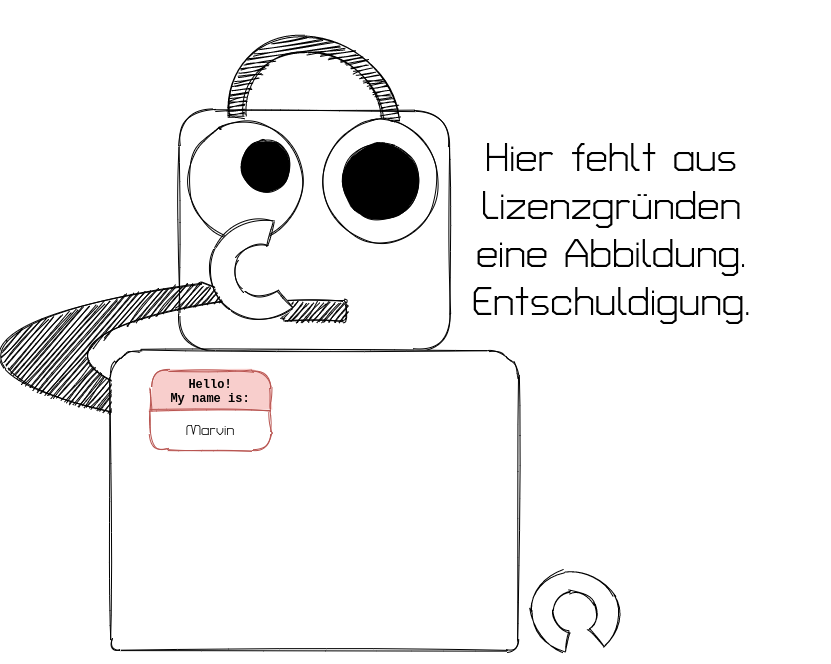
\includegraphics[width=200pt]{imgs/copyright} 

}

\caption{'Inclusion of the Other in the Self'-Skala aus @aronInclusionOtherSelf1992}\label{fig:unnamed-chunk-89}
\end{figure}

\hypertarget{guxfcte-von-operationalisierungen}{%
\section{Güte von Operationalisierungen}\label{guxfcte-von-operationalisierungen}}

\hypertarget{qualituxe4ts-merkmale-von-operationalisierungen}{%
\subsection{(Qualitäts-)Merkmale von Operationalisierungen:}\label{qualituxe4ts-merkmale-von-operationalisierungen}}

\begin{itemize}
\item
  \textbf{\emph{Divergenz}:} Ein theoretisches Konstrukt kann durch mehrere Indikatoren operationalisiert werden, wobei jeweils verschiedene Aspekte des Konstrukts unterschiedlich gut abgebildet werden.
\item
  \textbf{\emph{Konvergenz} :} Ein empirischer Indikator operationalisiert gleichzeitig verschiedene Aspekte mehrerer Konstrukte, wobei manche besser abgebildet werden als andere.
\end{itemize}

\begin{center}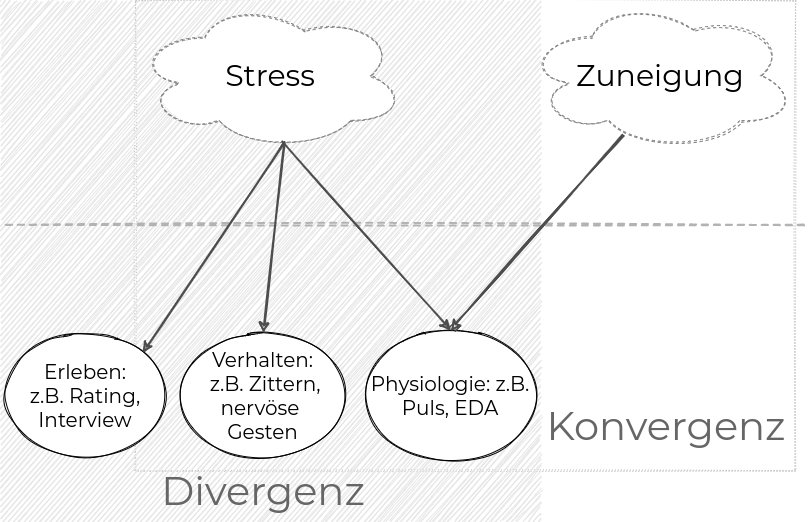
\includegraphics[width=200pt]{imgs/operartionalisierung_konvdiv} \end{center}

\hypertarget{qualituxe4ts-merkmale-von-operationalisierungen-1}{%
\subsection{(Qualitäts-)Merkmale von Operationalisierungen:}\label{qualituxe4ts-merkmale-von-operationalisierungen-1}}

\begin{itemize}
\item
  \textbf{\emph{Sensitivität} : } „Empfindlichkeit`` mit der ein Indikator das gemeinte Konstrukt anzeigt,
  unabhängig davon ob er zusätzlich auch weitere Konstrukte anzeigt.
\item
  \textbf{\emph{Selektivität/Spezifität} : } „Präzision`` mit der ein Indikator ausschließlich das gemeinte Konstrukt
  und nicht auch weitere Konstrukte anzeigt.
\end{itemize}

\(\rightarrow\) Eine Hypothese bewährt sich um so stärker, bzw. kann um so weiter generalisiert werden, je
mehr unterschiedliche Operationalisierungen für ihre Kernkonstrukte verwendet werden.
„Funktioniert`` nur eine bestimmte Operationalisierung ist oft fraglich welches Konstrukt eigentlich
dahinter steht.

\hypertarget{sensitivituxe4t-spezifituxe4t}{%
\subsection{Sensitivität / Spezifität}\label{sensitivituxe4t-spezifituxe4t}}

 
  \providecommand{\huxb}[2]{\arrayrulecolor[RGB]{#1}\global\arrayrulewidth=#2pt}
  \providecommand{\huxvb}[2]{\color[RGB]{#1}\vrule width #2pt}
  \providecommand{\huxtpad}[1]{\rule{0pt}{#1}}
  \providecommand{\huxbpad}[1]{\rule[-#1]{0pt}{#1}}

\begin{table}[ht]
\begin{centerbox}
\begin{threeparttable}
\captionsetup{justification=centering,singlelinecheck=off}
\caption{\label{tab:unnamed-chunk-91} }
 \setlength{\tabcolsep}{0pt}
\begin{tabularx}{1\textwidth}{p{0.33\textwidth} p{0.33\textwidth} p{0.33\textwidth}}


\hhline{}
\arrayrulecolor{black}

\multicolumn{1}{!{\huxvb{0, 0, 0}{0}}b{0.33\textwidth}!{\huxvb{0, 0, 0}{0}}}{\hspace{6pt}\parbox[t]{0.33\textwidth-6pt-6pt}{\huxtpad{6pt + 1em}\centering \huxbpad{6pt}}\rule{0pt}{0.2\textheight}} &
\multicolumn{1}{b{0.33\textwidth}!{\huxvb{0, 0, 0}{0}}}{\hspace{6pt}\parbox[t]{0.33\textwidth-6pt-6pt}{\huxtpad{6pt + 1em}\centering krank\huxbpad{6pt}}\rule{0pt}{0.2\textheight}} &
\multicolumn{1}{b{0.33\textwidth}!{\huxvb{0, 0, 0}{0}}}{\hspace{6pt}\parbox[t]{0.33\textwidth-6pt-6pt}{\huxtpad{6pt + 1em}\centering nicht krank\huxbpad{6pt}}\rule{0pt}{0.2\textheight}} \tabularnewline[-0.5pt]


\hhline{>{\huxb{255, 255, 255}{0.4}}->{\huxb{0, 0, 0}{0.4}}->{\huxb{0, 0, 0}{0.4}}-}
\arrayrulecolor{black}

\multicolumn{1}{!{\huxvb{0, 0, 0}{0}}m{0.33\textwidth}!{\huxvb{0, 0, 0}{0.4}}}{\hspace{6pt}\parbox[c]{0.33\textwidth-6pt-6pt}{\huxtpad{6pt + 1em}\centering Test positiv\huxbpad{6pt}}\rule{0pt}{0.4\textheight}} &
\multicolumn{1}{m{0.33\textwidth}!{\huxvb{0, 0, 0}{0.4}}}{\hspace{6pt}\parbox[c]{0.33\textwidth-6pt-6pt}{\huxtpad{6pt + 1em}\centering richtig positiv\huxbpad{6pt}}\rule{0pt}{0.4\textheight}} &
\multicolumn{1}{m{0.33\textwidth}!{\huxvb{0, 0, 0}{0.4}}}{\hspace{6pt}\parbox[c]{0.33\textwidth-6pt-6pt}{\huxtpad{6pt + 1em}\centering falsch positiv\huxbpad{6pt}}\rule{0pt}{0.4\textheight}} \tabularnewline[-0.5pt]


\hhline{>{\huxb{255, 255, 255}{0.4}}->{\huxb{0, 0, 0}{0.4}}|>{\huxb{0, 0, 0}{0.4}}->{\huxb{0, 0, 0}{0.4}}-}
\arrayrulecolor{black}

\multicolumn{1}{!{\huxvb{0, 0, 0}{0}}m{0.33\textwidth}!{\huxvb{0, 0, 0}{0.4}}}{\hspace{6pt}\parbox[c]{0.33\textwidth-6pt-6pt}{\huxtpad{6pt + 1em}\centering Test negativ\huxbpad{6pt}}\rule{0pt}{0.4\textheight}} &
\multicolumn{1}{m{0.33\textwidth}!{\huxvb{0, 0, 0}{0.4}}}{\hspace{6pt}\parbox[c]{0.33\textwidth-6pt-6pt}{\huxtpad{6pt + 1em}\centering falsch negativ\huxbpad{6pt}}\rule{0pt}{0.4\textheight}} &
\multicolumn{1}{m{0.33\textwidth}!{\huxvb{0, 0, 0}{0.4}}}{\hspace{6pt}\parbox[c]{0.33\textwidth-6pt-6pt}{\huxtpad{6pt + 1em}\centering richtig negativ\huxbpad{6pt}}\rule{0pt}{0.4\textheight}} \tabularnewline[-0.5pt]


\hhline{>{\huxb{255, 255, 255}{0.4}}->{\huxb{0, 0, 0}{0.4}}|>{\huxb{0, 0, 0}{0.4}}->{\huxb{0, 0, 0}{0.4}}-}
\arrayrulecolor{black}
\end{tabularx}
\end{threeparttable}\par\end{centerbox}

\end{table}
 

Sensitivität\(:= \frac{richtig\hspace{1mm} positiv}{krank}\)

Spezifität\(:= \frac{richtig\hspace{1mm} negativ}{nicht \hspace{1mm} krank}\)

\href{https://www.youtube.com/watch?v=czzrPQIg54Q}{Sehr gute, aktuelle Erklärung von Dr.~Mai Thi Nguyen-Kim}

\hypertarget{exkurs-klassische-testtheorie-validituxe4t-reliabilituxe4t-objektivituxe4t}{%
\subsection{Exkurs klassische Testtheorie: Validität, Reliabilität, Objektivität}\label{exkurs-klassische-testtheorie-validituxe4t-reliabilituxe4t-objektivituxe4t}}

Die Begriffe \emph{Validität}, \emph{Reliabilität} und \emph{Objektivität} nennt man die \textbf{Hauptgütekriterien} der klassischen Testtheorie. \bigskip

\begin{itemize}
\item
  \textbf{Reliabilität}: Sind meine Messergebnisse unabhängig von Störeinflüssen?
\item
  \textbf{Validität}: Messe ich das theoretische Konstrukt, das ich messen möchte?
\item
  \textbf{Objektivität}: Sind die Ergebnisse meines Messinstruments unabhängig von der Person, die es anwendet?
\end{itemize}

\hypertarget{validituxe4ten-bei-experimenten}{%
\subsection{Validitäten bei Experimenten}\label{validituxe4ten-bei-experimenten}}

\hypertarget{konstruktvalidituxe4t}{%
\subsubsection{Konstruktvalidität:}\label{konstruktvalidituxe4t}}

Gibt an, inwieweit UVn und AVn so operationalisiert sind, dass sie die jeweiligen psychologischen
Konstrukte möglichst zutreffend repräsentieren und mit bestehenden Konstruktdefinitionen und
Theorien übereinstimmen.

\hypertarget{inferenzstatistische-validituxe4t}{%
\subsubsection{Inferenzstatistische Validität:}\label{inferenzstatistische-validituxe4t}}

Gibt an, inwieweit die gewählten statistischen Verfahren geeignet sind, um von einer Stichprobe
auf Variablen in der Population zu schließen (gefährdet bei Verletzung der Voraussetzungen)

\hypertarget{interne-validituxe4t}{%
\subsubsection{Interne Validität:}\label{interne-validituxe4t}}

Gibt an, inwieweit die Veränderungen der AV auf die Manipulation der UVn zurückgeführt und
mögliche Alternativerklärungen durch Störeinflüsse ausgeschlossen werden können.

\hypertarget{externe-validituxe4t}{%
\subsubsection{Externe Validität:}\label{externe-validituxe4t}}

Gibt an, inwieweit die Untersuchungsergebnisse übertragbar (generalisierbar) sind
von der Stichprobe auf die Population (Repräsentativität)
von der Laborsituation auf natürliche Situationen (ökologische Validität)

\hypertarget{wie-kuxf6nnte-man-intelligenz-messen}{%
\subsection{Wie könnte man Intelligenz messen?}\label{wie-kuxf6nnte-man-intelligenz-messen}}

\begin{table}[H]
\centering
\begin{tabular}[t]{l>{}l>{}l}
\toprule
  & niedrige Validität & hohe Validität\\
\midrule
hohe Reliabilität & [\textasciicircum{}1]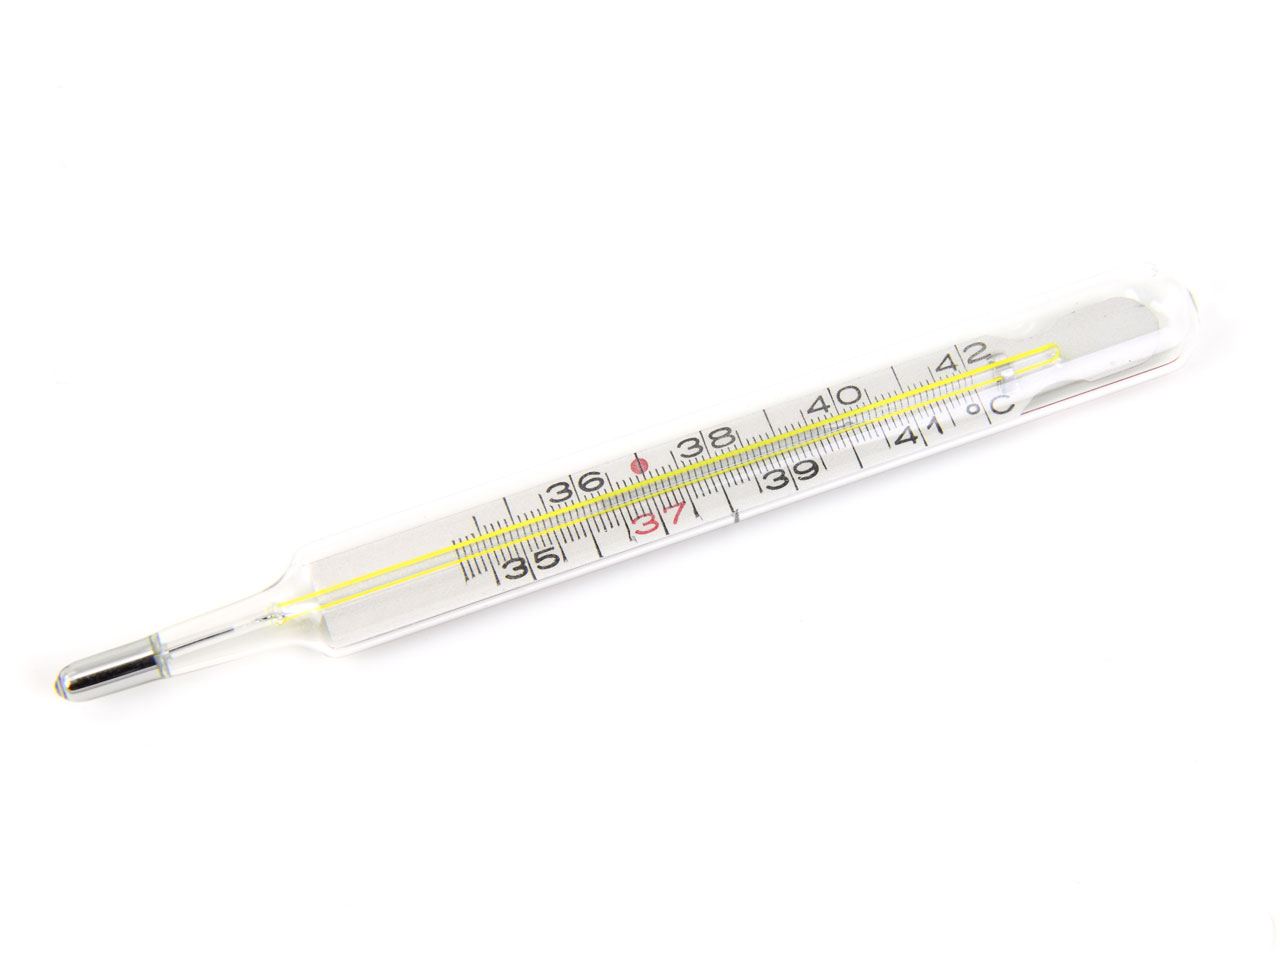
\includegraphics[width=1.5in, height=1.5in]{imgs/thermo.jpg} & 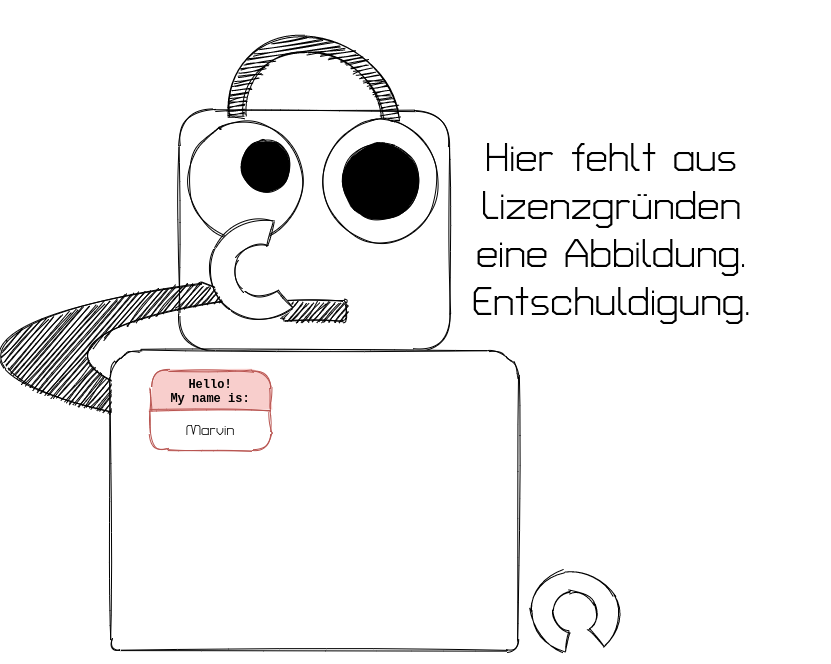
\includegraphics[width=1.5in, height=1.5in]{imgs/copyright.png}\\
niedrige Reliabilität & [\textasciicircum{}2]\includegraphics[width=1.5in, height=1.5in]{imgs/frog.jpg} & [\textasciicircum{}3]\includegraphics[width=1.5in, height=1.5in]{imgs/kitty.png}\\
\bottomrule
\end{tabular}
\end{table}

\hypertarget{validituxe4t-in-experimenten}{%
\subsection{Validität in Experimenten}\label{validituxe4t-in-experimenten}}

\begin{center}\includegraphics[width=200pt]{imgs/validitaeten} \end{center}

\hypertarget{operationalisierungsmethoden}{%
\section{Operationalisierungsmethoden}\label{operationalisierungsmethoden}}

\hypertarget{operationalisierung-der-uv}{%
\subsection{Operationalisierung der UV}\label{operationalisierung-der-uv}}

\hypertarget{externe-einfluxfcsse-externe-uv}{%
\subsubsection{Externe Einflüsse / externe UV:}\label{externe-einfluxfcsse-externe-uv}}

\begin{itemize}
\tightlist
\item
  Sind meist beobachtungsnah und lassen sich daher relativ leicht operationalisieren.
\item
  Beispiele:

  \begin{itemize}
  \tightlist
  \item
    „Lärm beeinflusst die Konzentrationsleistung.``
  \item
    „Die Luminanz des Hintergrundes beeinflusst die wahrgenommene Helligkeit des Objektes``
  \end{itemize}
\end{itemize}

\hypertarget{interne-psychologische-konstrukte-interne-uvn}{%
\subsubsection{Interne psychologische Konstrukte / interne UVn:}\label{interne-psychologische-konstrukte-interne-uvn}}

\begin{itemize}
\tightlist
\item
  Sind meist beobachtungsfern und müssen aufwendiger und indirekter operationalisiert werden.
\item
  Beispiele:

  \begin{itemize}
  \tightlist
  \item
    „Motivation beeinflusst die Konzentrationsleistung.``
  \item
    „Das Vorwissen über ein Objekt beeinflusst seine wahrgenommene Helligkeit.``
  \end{itemize}
\end{itemize}

\hypertarget{operationalisierung-der-uv-1}{%
\subsection{Operationalisierung der UV}\label{operationalisierung-der-uv-1}}

Konkret werden oft komplexe Versuchsanordnungen verwendet um bestimmte UV Stufen zu
operationalisieren. Handelt es sich bei der UV um ein \textbf{internes psychologisches Konstrukt}, so kann
dieses natürlich nur \textbf{indirekt} über die \textbf{Auswirkung externer Manipulationen} (und \textbf{unter Annahme
von Hilfshypothesen!}) operationalisiert werden.

Hierzu werden \textbf{Umgebungsbedingungen, Reize, Instruktionen, Aufgaben,} etc. entsprechend variiert.

\hypertarget{operationalisierung-der-av-mauxdfe-der-verhaltenswissenschaft-psychologie}{%
\subsection{Operationalisierung der AV: Maße der Verhaltenswissenschaft (Psychologie)}\label{operationalisierung-der-av-mauxdfe-der-verhaltenswissenschaft-psychologie}}

\textbf{Verhaltensbeobachtung:} Das Verhalten der VP wird direkt beobachtet und für das Konstrukt
relevantes Verhalten wird möglichst objektiv erfasst.

\textbf{Befragung:} Die VP antwortet mündlich (Interview) oder schriftlich (Fragebogen) auf ihr gestellte
Fragen. Die Fragen können mehr (Ankreuzen, Ratingskalen) oder weniger (freies Antwortformat)
strukturiert sein.

\textbf{Test:} Der VP werden unter standardisierten Bedingungen standardisierte Reize (Bilder, Töne,
Aufgaben, etc.) vorgegeben, auf welche die VP reagieren muss (Benennen, Knopf drücken, komplexe
Aufgabe lösen, etc.). Die Reaktionen können ggf. mit großen Normstichproben verglichen werden.

\textbf{Analyse von Verhaltensspuren:} Indirekte Spuren des Verhaltens der VP (Zeichnungen, Briefe, Fotos,
Tagebücher, Nutzungsspuren, Cookies, Bewegungsprofile, etc.) werden ausgewertet.

\textbf{Spezielle Mess- und Beobachtungsgeräte:} z.B. Messung der Augenbewegungen, Fixationen,
Sakkaden und Pupillenreaktionen mittels Eye-Tracking

\hypertarget{uxfcbung}{%
\subsection{Übung}\label{uxfcbung}}

Gibt's im Olat

\hypertarget{literatur-1}{%
\subsection{Literatur}\label{literatur-1}}

\hypertarget{experimentelle-versuchspluxe4ne}{%
\chapter{Experimentelle Versuchspläne}\label{experimentelle-versuchspluxe4ne}}

\hypertarget{organisatorisches-5}{%
\section{Organisatorisches}\label{organisatorisches-5}}

\hypertarget{semesterplan-6}{%
\subsection{Semesterplan}\label{semesterplan-6}}

\begin{tabular}[t]{rll}
\toprule
Sitzung & Datum & Sitzungstitel\\
\midrule
1 & 02.11.2020 & Warum wissenschaftliche Psychologie\\
2 & 28.11.2020
29.11.2020 & Hypothesen und der Prozess der Hypothesenprüfung\\
3 & 28.11.2020
29.11.2020 & Experimentelles Vorgehen\\
4 & 28.11.2020
29.11.2020 & Literaturrecherche\\
5 & 28.11.2020
29.11.2020 & Operationalisieren und Messen\\
\addlinespace
6 & 12.12.2020
13.12.2020 & Experimentelle Versuchspläne\\
7 & 12.12.2020
13.12.2020 & Störvariablen im Experiment\\
8 & 12.12.2020
13.12.2020 & Nicht-experimentelle Versuchspläne\\
9 & 12.12.2020
13.12.2020 & Material und Stichprobe\\
10 & 23.1.2021
24.1.2021 & Auswertung, Darstellung und Interpretation\\
\addlinespace
11 & 23.1.2021
24.1.2021 & Ethische Probleme im Versuch\\
12 & 23.1.2021
24.1.2021 & Publikationsprozess\\
13 & wird noch bekannt gegeben & Vorstellung der Gruppenarbeiten\\
14 & wird noch bekannt gegeben & Klausurvorbereitung\\
\bottomrule
\end{tabular}

\hypertarget{wiederholung-4}{%
\section{Wiederholung}\label{wiederholung-4}}

\hypertarget{operationalisieren}{%
\subsection{Operationalisieren}\label{operationalisieren}}

\begin{center}\includegraphics[width=200pt]{imgs/operartionalisierung} \end{center}

\hypertarget{qualituxe4ts-merkmale-von-operationalisierungen-2}{%
\subsection{(Qualitäts-)Merkmale von Operationalisierungen:}\label{qualituxe4ts-merkmale-von-operationalisierungen-2}}

\begin{itemize}
\tightlist
\item
  \textbf{\emph{Divergenz}:} Ein theoretisches Konstrukt kann durch mehrere Indikatoren operationalisiert werden, wobei jeweils verschiedene Aspekte des Konstrukts unterschiedlich gut abgebildet werden.
\item
  \textbf{\emph{Konvergenz} :} Ein empirischer Indikator operationalisiert gleichzeitig verschiedene Aspekte mehrerer Konstrukte, wobei manche besser abgebildet werden als andere.
\item
  \textbf{\emph{Sensitivität} : } „Empfindlichkeit`` mit der ein Indikator das gemeinte Konstrukt anzeigt,
  unabhängig davon ob er zusätzlich auch weitere Konstrukte anzeigt.
\item
  \textbf{\emph{Selektivität/Spezifität} : } „Präzision`` mit der ein Indikator ausschließlich das gemeinte Konstrukt
  und nicht auch weitere Konstrukte anzeigt. \smallskip \newline
\end{itemize}

\(\rightarrow\) Eine Hypothese bewährt sich um so stärker, bzw. kann um so weiter generalisiert werden, je
mehr unterschiedliche Operationalisierungen für ihre Kernkonstrukte verwendet werden.
„Funktioniert`` nur eine bestimmte Operationalisierung ist oft fraglich welches Konstrukt eigentlich
dahinter steht.

\hypertarget{validituxe4ten-bei-experimenten-1}{%
\subsection{Validitäten bei Experimenten}\label{validituxe4ten-bei-experimenten-1}}

\hypertarget{konstruktvalidituxe4t-1}{%
\subsubsection{Konstruktvalidität:}\label{konstruktvalidituxe4t-1}}

Gibt an, inwieweit UVn und AVn so operationalisiert sind, dass sie die jeweiligen psychologischen
Konstrukte möglichst zutreffend repräsentieren und mit bestehenden Konstruktdefinitionen und
Theorien übereinstimmen.

\hypertarget{inferenzstatistische-validituxe4t-1}{%
\subsubsection{Inferenzstatistische Validität:}\label{inferenzstatistische-validituxe4t-1}}

Gibt an, inwieweit die gewählten statistischen Verfahren geeignet sind, um von einer Stichprobe
auf Variablen in der Population zu schließen (gefährdet bei Verletzung der Voraussetzungen)

\hypertarget{interne-validituxe4t-1}{%
\subsubsection{Interne Validität:}\label{interne-validituxe4t-1}}

Gibt an, inwieweit die Veränderungen der AV auf die Manipulation der UVn zurückgeführt und
mögliche Alternativerklärungen durch Störeinflüsse ausgeschlossen werden können.

\hypertarget{externe-validituxe4t-1}{%
\subsubsection{Externe Validität:}\label{externe-validituxe4t-1}}

Gibt an, inwieweit die Untersuchungsergebnisse übertragbar (generalisierbar) sind
von der Stichprobe auf die Population (Repräsentativität)
von der Laborsituation auf natürliche Situationen (ökologische Validität)

\hypertarget{versuchspluxe4ne}{%
\section{Versuchspläne}\label{versuchspluxe4ne}}

\hypertarget{wozu-uxfcberhaupt-2}{%
\subsection{Wozu überhaupt?}\label{wozu-uxfcberhaupt-2}}

\begin{cols}

\begin{col}{0.30\textwidth}

\begin{center}\includegraphics[width=150pt]{imgs/hypothesen_vp} \end{center}

\end{col}

\begin{col}{0.68\textwidth}

\textbf{Versuchsplan/-design:}

Strukturelles Schema der geplanten Ver-
suchsdurchführung zur übersichtlichen
Darstellung von:

\begin{itemize}
\item
  wesentlichem Ablauf der Untersuchung
\item
  UVs, AVs, vorgenommene SV-Kontrollen
\item
  Versuchspersonengruppierung
\end{itemize}

\end{col}

\end{cols}

\hypertarget{einfaktorielle-versuchspluxe4ne}{%
\subsection{Einfaktorielle Versuchspläne}\label{einfaktorielle-versuchspluxe4ne}}

\hypertarget{grafische-darstellung-von-versuchspluxe4nen}{%
\subsubsection{Grafische Darstellung von Versuchsplänen}\label{grafische-darstellung-von-versuchspluxe4nen}}

\begin{center}\includegraphics[width=166.666666666667pt]{imgs/plan1} \end{center}

\begin{center}\includegraphics[width=100pt]{imgs/plan2} \end{center}

\begin{center}\includegraphics[width=250pt]{imgs/plan3} \end{center}

\hypertarget{randomisierungspluxe4ne}{%
\subsubsection{Randomisierungspläne}\label{randomisierungspluxe4ne}}

\begin{center}\includegraphics[width=250pt]{imgs/plan4} \end{center}

\begin{itemize}
\tightlist
\item
  Zufällige Aufteilung der VP auf \(\geq 2\) Gruppen
\item
  Gruppenzugehörigkeit \(\Leftrightarrow\) UV-Stufe

  \begin{itemize}
  \tightlist
  \item
    UV ist unabhängig / Zwischen-Gruppen-Faktor
  \end{itemize}
\end{itemize}

\begin{cols}

\begin{col}{0.48\textwidth}

\textbf{Vorteile}

\begin{itemize}
\item
  Einfache Umsetzung
\item
  Organismusvariablen werden zufällig auf Bedingungen aufgeteilt, damit kontrolliert
\end{itemize}

\end{col}

\begin{col}{0.48\textwidth}

\textbf{Nachteile}

\begin{itemize}
\item
  Erfordert aureichend große Stichprobe
\item
  Zufallsvarianz wird künstlich erhöht
\end{itemize}

\end{col}

\end{cols}

\hypertarget{messwiederholungspluxe4ne}{%
\subsubsection{Messwiederholungspläne}\label{messwiederholungspluxe4ne}}

\begin{center}\includegraphics[width=250pt]{imgs/plan5} \end{center}

\begin{itemize}
\tightlist
\item
  Mehrfache Messung der \emph{selben} VP in \(\geq 2\) Bedingungen
\item
  Bedingung \(\Leftrightarrow\) UV-Stufe

  \begin{itemize}
  \tightlist
  \item
    UV ist abhängig / Intra-Gruppen-Faktor
  \end{itemize}
\end{itemize}

\begin{cols}

\begin{col}{0.48\textwidth}

\textbf{Vorteile}

\begin{itemize}
\item
  Kontrolliert Organismusvariablen durch ``konstanthalten'' in VP
\item
  Reduziert Zufallsvarianz
\item
  Reduziert nötige Stichprobengröße
\item
  Vorher-Nachher-Aussagen möglich
\item
  zeigt ggf. Baseline-Unterschiede auf
\end{itemize}

\end{col}

\begin{col}{0.48\textwidth}

\textbf{Nachteile}

\begin{itemize}
\item
  Reihenfolge-, Test-, Reaktivitäts- und Ermüdungseffekte usw. möglich
\item
  Aufwand/Kosten können durch Mehrfachmessung erhöht werden
\end{itemize}

\end{col}

\end{cols}

\hypertarget{blockversuchspluxe4ne}{%
\subsubsection{Blockversuchspläne}\label{blockversuchspluxe4ne}}

\begin{center}\includegraphics[width=250pt]{imgs/plan6} \end{center}

\begin{itemize}
\tightlist
\item
  Gezielte Aufteilung der VPn in \(\geq 2\) Gruppen nach Ausprägung einer SV
\item
  `SV-Stufe' \(\Leftrightarrow\) UV-Stufe

  \begin{itemize}
  \tightlist
  \item
    UV ist unabhängig / Zwischen-Gruppen-Faktor (bei \emph{sehr} strengem ``Matching'' können sich auch Abhängigkeiten geben.)
  \end{itemize}
\end{itemize}

\begin{cols}

\begin{col}{0.48\textwidth}

\textbf{Vorteile}

\begin{itemize}
\item
  starke Kontrolle einer SV, auch bei kleinem N
\item
  reduzierte Zufallsvarianz
\end{itemize}

\end{col}

\begin{col}{0.48\textwidth}

\textbf{Nachteile}

\begin{itemize}
\item
  SV muss bekannt und messbar sein, um zur Blockbildung genutzt werden zu können
\item
  mehr als ein Blockbildungsfaktor führt zu hohem technischem und finanziellem Aufwand
\end{itemize}

\end{col}

\end{cols}

\hypertarget{mehrfaktorielle-versuchspluxe4ne}{%
\subsection{Mehrfaktorielle Versuchspläne}\label{mehrfaktorielle-versuchspluxe4ne}}

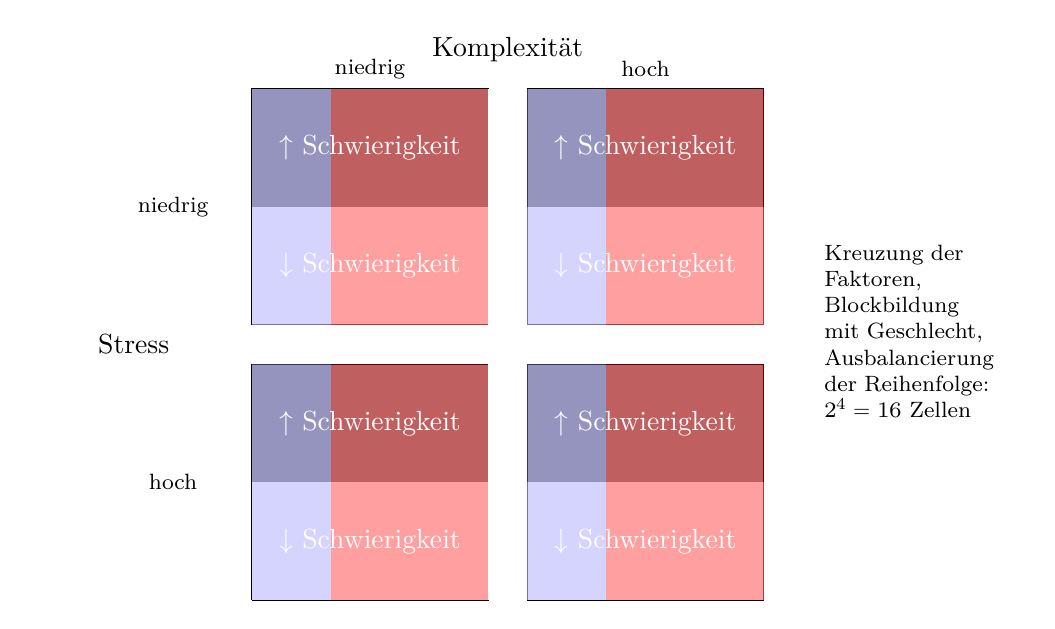
\begin{tikzpicture}
\tikzset{
    mytext/.style={text width=7em,align=center},
    mylabel/.style={text width=7em,align=center, font=\footnotesize}
}

  \draw (1,1) -- (4,1) -- (4,4) -- (1,4) -- (1,1);
  \draw (4.5,4.5) -- (7.5,4.5) -- (7.5,7.5) -- (4.5,7.5) -- (4.5,4.5);
  \draw (1,4.5) -- (4,4.5) -- (4,7.5) -- (1,7.5) -- (1,4.5);
  \draw (4.5,1) -- (4.5,4) -- (7.5,4) -- (7.5,1) -- (4.5,1);
  \fill [Red, opacity=.5] (2,1) rectangle (4,7.5);
  \fill [Red, opacity=.5] (5.5,1) rectangle (7.5,7.5);
  \fill [Blue, opacity=.5] (1,1) rectangle (2,7.5);
  \fill [Blue, opacity=.5] (4.5,1) rectangle (5.5,7.5);
  
  
  \fill [White, opacity=.25] (1,1) rectangle (7.5,2.5);
  \fill [White, opacity=.25] (1,4.5) rectangle (7.5,6);
  \fill [Black, opacity=.25] (1,2.5) rectangle (7.5,4);
  \fill [Black, opacity=.25] (1,6) rectangle (7.5,7.5);
  

  \fill [White, opacity=1] (1,4) rectangle (7.5,4.5);
  \fill [White, opacity=1] (4,1) rectangle (4.5,7.5);
  
  \node[mytext] at (2.5,3.25) {\textcolor{White}{$\uparrow$ Schwierigkeit}};
  \node[mytext] at (2.5,1.75) {\textcolor{White}{$\downarrow$ Schwierigkeit}};
    \node[mytext] at (2.5,6.75) {\textcolor{White}{$\uparrow$ Schwierigkeit}};
  \node[mytext] at (2.5,5.25) {\textcolor{White}{$\downarrow$ Schwierigkeit}};
    \node[mytext] at (6,3.25) {\textcolor{White}{$\uparrow$ Schwierigkeit}};
  \node[mytext] at (6,1.75) {\textcolor{White}{$\downarrow$ Schwierigkeit}};
    \node[mytext] at (6,6.75) {\textcolor{White}{$\uparrow$ Schwierigkeit}};
  \node[mytext] at (6,5.25) {\textcolor{White}{$\downarrow$ Schwierigkeit}};
  
    \node[mylabel] at (2.5,7.75) {niedrig};
  \node[mylabel] at (6,7.75) {hoch};
  \node[mylabel] at (0,6) {niedrig};
  \node[mylabel] at (0,2.5) {hoch};
  \node[mytext] at (-0.5,4.25) {Stress};
  \node[mytext] at (4.25,8) {Komplexität};
  \node[mylabel] at(9.5, 4.25) {Kreuzung der \newline Faktoren, \newline Blockbildung \newline mit Geschlecht, \newline Ausbalancierung \newline der Reihenfolge: \newline $2^4=16$ Zellen \newline};
\end{tikzpicture}

\hypertarget{uxfcbung-1}{%
\subsection{Übung}\label{uxfcbung-1}}

Beantworten Sie für die ausgeteilten Artikel folgende Frage- \& Aufgabestellung:

\begin{itemize}
\tightlist
\item
  Um welche Art von Studie handelt es sich bei der beschriebenen wissenschaftlichen Untersuchung?

  \begin{itemize}
  \tightlist
  \item
    Experiment, Quasiexperiment, \ldots{}
  \end{itemize}
\item
  Was könnte eine mögliche Hypothese sein, die der Studie zugrunde liegt?
\item
  Gibt es in der Studie mindestens eine UV? Wenn ja, was sind UV(s), AV(s), evtl. kontrollierte Störvariablen/nicht kontrollierte Störvariablen? Wenn nicht, welche anderen Variablen wurden wozu erhoben?

  \begin{itemize}
  \tightlist
  \item
    Wenn genauer beschrieben, wie wurden diese operationalisiert?
  \item
    Ist/Sind die etwaigen UV(s) abhängig oder unabhängig?
  \end{itemize}
\item
  Stellen Sie das Studiendesign wenn möglich tabellarisch dar.
\end{itemize}

\hypertarget{hausaufgabe-1}{%
\subsection{Hausaufgabe}\label{hausaufgabe-1}}

Huber, Kapitel 6 \& 7, Seiten 169 - 193

\hypertarget{stuxf6rvariablen}{%
\chapter{Störvariablen}\label{stuxf6rvariablen}}

\hypertarget{organisatorisches-6}{%
\section{Organisatorisches}\label{organisatorisches-6}}

\hypertarget{semesterplan-7}{%
\subsection{Semesterplan}\label{semesterplan-7}}

\begin{tabular}[t]{rll}
\toprule
Sitzung & Datum & Sitzungstitel\\
\midrule
1 & 02.11.2020 & Warum wissenschaftliche Psychologie\\
2 & 28.11.2020
29.11.2020 & Hypothesen und der Prozess der Hypothesenprüfung\\
3 & 28.11.2020
29.11.2020 & Experimentelles Vorgehen\\
4 & 28.11.2020
29.11.2020 & Literaturrecherche\\
5 & 28.11.2020
29.11.2020 & Operationalisieren und Messen\\
\addlinespace
6 & 12.12.2020
13.12.2020 & Experimentelle Versuchspläne\\
7 & 12.12.2020
13.12.2020 & Störvariablen im Experiment\\
8 & 12.12.2020
13.12.2020 & Nicht-experimentelle Versuchspläne\\
9 & 12.12.2020
13.12.2020 & Material und Stichprobe\\
10 & 23.1.2021
24.1.2021 & Auswertung, Darstellung und Interpretation\\
\addlinespace
11 & 23.1.2021
24.1.2021 & Ethische Probleme im Versuch\\
12 & 23.1.2021
24.1.2021 & Publikationsprozess\\
13 & wird noch bekannt gegeben & Vorstellung der Gruppenarbeiten\\
14 & wird noch bekannt gegeben & Klausurvorbereitung\\
\bottomrule
\end{tabular}

\hypertarget{wiederholung-5}{%
\section{Wiederholung}\label{wiederholung-5}}

\hypertarget{mehrfaktorielle-versuchspluxe4ne-1}{%
\subsection{Mehrfaktorielle Versuchspläne}\label{mehrfaktorielle-versuchspluxe4ne-1}}

\hypertarget{varianz---freund-und-feind}{%
\section{Varianz - Freund und Feind}\label{varianz---freund-und-feind}}

\hypertarget{varianz-der-abhuxe4ngigen-variable}{%
\subsection{Varianz der abhängigen Variable}\label{varianz-der-abhuxe4ngigen-variable}}

\begin{cols}

\begin{col}{0.48\textwidth}

\textbf{Sehr wenig Varianz}

Graue Flecken an den Kreuzungen


\begin{tikzpicture}
  \fill [Black] (0,0) rectangle (1.2,1.2);
  \fill [Black] (0,1.5) rectangle (1.2,2.7);
  \fill [Black] (0,3) rectangle (1.2,4.2);


  \fill [Black] (1.5,0) rectangle (2.7,1.2);
  \fill [Black] (1.5,1.5) rectangle (2.7,2.7);
  \fill [Black] (1.5,3) rectangle (2.7,4.2);

  \fill [Black] (3,0) rectangle (4.2,1.2);
  \fill [Black] (3,1.5) rectangle (4.2,2.7);
  \fill [Black] (3,3) rectangle (4.2,4.2);
\end{tikzpicture}

\end{col}

\begin{col}{0.48\textwidth}

\textbf{Sehr viel Varianz}

Die Attraktivität dieses Mannes

\begin{center}\includegraphics[width=66.6666666666667pt]{imgs/copyright} \end{center}

\end{col}

\end{cols}

\hypertarget{varianzanteile}{%
\subsection{Varianzanteile}\label{varianzanteile}}

\begin{center}\includegraphics[width=200pt]{imgs/varianzen} \end{center}

\hypertarget{beispiel-evaluation-einer-neuen-therapie-fuxfcr-depression}{%
\subsection{Beispiel: Evaluation einer neuen Therapie für Depression}\label{beispiel-evaluation-einer-neuen-therapie-fuxfcr-depression}}

Wir überprüfen die Wirkung einer neuen Therapie

\begin{itemize}
\item
  Unabhängige Variable: Interventionsform (Warten vs.~Therapie)
\item
  Abhängige Variable: Wert im Depressionsfragebogen nach 5 Wochen
\end{itemize}

\begin{center}\includegraphics[width=200pt]{Versuchsplanung_WS20_files/figure-latex/unnamed-chunk-122-1} \end{center}

\href{https://mbrede.shinyapps.io/VPlanung/}{Varianzzerlegung}

\hypertarget{stuxf6rvariablen-1}{%
\section{Störvariablen}\label{stuxf6rvariablen-1}}

\hypertarget{konfundierung}{%
\subsection{Konfundierung}\label{konfundierung}}

\textbf{Konfundierung:} Kovariieren die Stufen einer UV und die Ausprägungen einer Störvariable, so
ist die UV mit der SV konfundiert. Die Wirkung der UV kann dann nicht mehr getrennt von der
Wirkung der SV gemessen werden.

Lässt sich eine Konfundierung nicht vermeiden, kann das Experiment nicht durchgeführt
werden, bzw. hat eine reduzierte Aussagekraft (je nach Schwere der Konfundierung).

Wird eine Konfundierung im nachhinein entdeckt, so ist das Experiment unbrauchbar, bzw.
kann nicht mehr im ursprünglichen Sinne interpretiert werden.

\hypertarget{arten-von-stuxf6rvariablen}{%
\subsection{Arten von Störvariablen}\label{arten-von-stuxf6rvariablen}}

\begin{itemize}
\item
  Variablen der Vp (Organismusvariablen)

  \begin{itemize}
  \tightlist
  \item
    Alter, Geschlecht, Extraversion, Intelligenz, Schulbildung, Vorerfahrungen mit psychologischen Untersuchungen oder mit verwendetem Testmaterial, etc.
  \end{itemize}
\end{itemize}

\hypertarget{kontrolle-von-stuxf6rvariablen-der-vpn}{%
\subsection{Kontrolle von Störvariablen der VPn}\label{kontrolle-von-stuxf6rvariablen-der-vpn}}

\textbf{Parallelisieren: }

\begin{itemize}
\tightlist
\item
  Störvariable ist im Mittel in allen Gruppen unter allen Bedingungen gleich
  ausgeprägt
\end{itemize}

\textbf{Matching:}

\begin{itemize}
\tightlist
\item
  In jede Gruppe / Bedingung wird einer von zwei Matchingpartnern gelost, der die
  gleichen Ausprägungen der Störvariablen hat
\end{itemize}

\textbf{Randomisieren:}

\begin{itemize}
\tightlist
\item
  Bei großen Gruppen geht man davon aus, dass bei zufälliger Verteilung der
  Personen auf Gruppen, Bedingungen die Störvariablen im Mittel gleich ausgeprägt sind
\end{itemize}

\textbf{Abhängige Desings}

\begin{itemize}
\tightlist
\item
  Abhängige UVs stellen eine sehr starke Art der Kontrolle von aus dem Organismus resultierenden Störvariablen dar
\end{itemize}

\hypertarget{stuxf6rvariablen-in-abhuxe4ngigen-designs}{%
\subsection{Störvariablen in abhängigen Designs}\label{stuxf6rvariablen-in-abhuxe4ngigen-designs}}

\begin{itemize}
\item
  Positionseffekte

  \begin{itemize}
  \item
    Ermüdungseffekte
  \item
    Test-Effekte
  \item
    Spontanheilung
  \item
    \ldots{}
  \end{itemize}
\item
  Carry-Over-Effekte

\begin{verbatim}
- Reaktivitäts-Effekte

- ...
\end{verbatim}
\end{itemize}

\begin{itemize}
\item
  (un-)vollständiges Ausbalancieren

  \begin{itemize}
  \tightlist
  \item
    funktioniert natürlich nicht bei Carry-Over-Effekten
  \end{itemize}
\item
  Eliminieren der Störvariable
\item
  Wechsel in unabhängiges Design
\end{itemize}

\hypertarget{arten-von-stuxf6rvariablen-1}{%
\subsection{Arten von Störvariablen}\label{arten-von-stuxf6rvariablen-1}}

\begin{itemize}
\item
  Variablen der Untersuchungssituation

  \begin{itemize}
  \item
    Versuchsleiter (VL): Geschlecht, Aussehen, Freundlichkeit, etc.
  \item
    Untersuchungsraum: Lichtverhältnisse, Lärmbelastung, Einrichtung, Größe, Farbwahl, etc.
  \item
    Instruktionen: Sprache, sprachliches Niveau, spezielle Formulierungen, etc.
  \item
    Testaufgaben: bestimmte Eigenschaften
  \item
    Fragen: Reihenfolge, Formulierungen, etc. etc.
  \end{itemize}
\end{itemize}

\hypertarget{kontrolle-von-stuxf6rvariablen-der-untersuchungssituation}{%
\subsection{Kontrolle von Störvariablen der Untersuchungssituation}\label{kontrolle-von-stuxf6rvariablen-der-untersuchungssituation}}

\textbf{Elimination:}

\begin{itemize}
\tightlist
\item
  Störvariable völlig ausschalten
\end{itemize}

\textbf{Konstanthalten:}

\begin{itemize}
\tightlist
\item
  Störvariable für Dauer des Versuches Konstant halten\\
  - Vorsicht: Generalisierbarkeit evtl. eingeschränkt
\end{itemize}

\textbf{Zufallsvariation:}

\begin{itemize}
\tightlist
\item
  Zufällige Zuteilung der Versuchsbedingungen auf `Störvariablen-Stufen'
\end{itemize}

\textbf{Einführung einer Kontrollgruppe:}

\begin{itemize}
\tightlist
\item
  Kontrolle von Veränderungen über die Zeit
\item
  Kontrolle von reaktiven Effekten der Vorhermessung
\end{itemize}

\hypertarget{arten-von-stuxf6rvariablen-2}{%
\subsection{Arten von Störvariablen}\label{arten-von-stuxf6rvariablen-2}}

\begin{itemize}
\item
  Variablen der sozialen (Untersuchungs-)Situation

  \begin{itemize}
  \item
    Versuchsleiter (VL): Organismusvariablen und Verhalten, Erwartungen.
  \item
    Versuchsperson (Vp): z.B. Erwartungen, Motivation Versuchssituation: Umgebung, andere Vpn\ldots{}
  \end{itemize}
\end{itemize}

\hypertarget{kontrolle-von-stuxf6rvariablen}{%
\subsection{Kontrolle von Störvariablen}\label{kontrolle-von-stuxf6rvariablen}}

\hypertarget{erwartungseffekte}{%
\subsubsection{Erwartungseffekte}\label{erwartungseffekte}}

\begin{itemize}
\item
  Rosenthal-Effekt
\item
  Placebo-Effekt
\item
  Aufforderungsvariablen
\item
  Soziale Erwünschtheit
\end{itemize}

Übung

\hypertarget{erwartungseffekte-1}{%
\subsubsection{Erwartungseffekte}\label{erwartungseffekte-1}}

\begin{itemize}
\item
  Nocebo-Effekt
\item
  Versagensangst
\item
  Andorra-Effekt
\item
  Hawthorne-Effekt
\end{itemize}

\hypertarget{kontrolle-von-stuxf6rvariablen-des-vl}{%
\subsection{Kontrolle von Störvariablen des VL}\label{kontrolle-von-stuxf6rvariablen-des-vl}}

\textbf{Standardisierung der Versuchsbedingungen:}

\begin{itemize}
\tightlist
\item
  festgelegte Abläufe und Verhaltensweisen verringern den Spielraum für Ausdruck von Erwartungen durch den VL
\end{itemize}

\textbf{Ausschalten des VL:}

\begin{itemize}
\tightlist
\item
  Verringerung des persönlichen Kontakts in kritischen Phasen des Experiments
\end{itemize}

\textbf{Training des VL:}

\begin{itemize}
\tightlist
\item
  Insbesondere Standardisierung von non-verbalem Ausdruck
\end{itemize}

\textbf{Manipulation der Erwartungen des VL:}

\begin{itemize}
\tightlist
\item
  bei mehreren VLn, kann die Erwartung des VL systematisch variiert und untersucht werden
\end{itemize}

\textbf{VL-Blindversuch und Doppelblindversuch:}

\begin{itemize}
\tightlist
\item
  kennt der VL die aktuelle Versuchsbedingung nicht, können seine Erwartungen nicht systematisch wirksam werden
\end{itemize}

\hypertarget{nicht-experimentelle-versuchspluxe4ne}{%
\chapter{nicht-experimentelle Versuchspläne}\label{nicht-experimentelle-versuchspluxe4ne}}

\hypertarget{organisatorisches-7}{%
\section{Organisatorisches}\label{organisatorisches-7}}

\hypertarget{semesterplan-8}{%
\subsection{Semesterplan}\label{semesterplan-8}}

\begin{tabular}[t]{rll}
\toprule
Sitzung & Datum & Sitzungstitel\\
\midrule
1 & 02.11.2020 & Warum wissenschaftliche Psychologie\\
2 & 28.11.2020
29.11.2020 & Hypothesen und der Prozess der Hypothesenprüfung\\
3 & 28.11.2020
29.11.2020 & Experimentelles Vorgehen\\
4 & 28.11.2020
29.11.2020 & Literaturrecherche\\
5 & 28.11.2020
29.11.2020 & Operationalisieren und Messen\\
\addlinespace
6 & 12.12.2020
13.12.2020 & Experimentelle Versuchspläne\\
7 & 12.12.2020
13.12.2020 & Störvariablen im Experiment\\
8 & 12.12.2020
13.12.2020 & Nicht-experimentelle Versuchspläne\\
9 & 12.12.2020
13.12.2020 & Material und Stichprobe\\
10 & 23.1.2021
24.1.2021 & Auswertung, Darstellung und Interpretation\\
\addlinespace
11 & 23.1.2021
24.1.2021 & Ethische Probleme im Versuch\\
12 & 23.1.2021
24.1.2021 & Publikationsprozess\\
13 & wird noch bekannt gegeben & Vorstellung der Gruppenarbeiten\\
14 & wird noch bekannt gegeben & Klausurvorbereitung\\
\bottomrule
\end{tabular}

\hypertarget{wiederholung-6}{%
\section{Wiederholung}\label{wiederholung-6}}

\hypertarget{varianz-der-abhuxe4ngigen-variable-1}{%
\subsection{Varianz der abhängigen Variable}\label{varianz-der-abhuxe4ngigen-variable-1}}

\begin{cols}

\begin{col}{0.48\textwidth}

\textbf{Sehr wenig Varianz}

Graue Flecken an den Kreuzungen


\begin{tikzpicture}
  \fill [Black] (0,0) rectangle (1.2,1.2);
  \fill [Black] (0,1.5) rectangle (1.2,2.7);
  \fill [Black] (0,3) rectangle (1.2,4.2);


  \fill [Black] (1.5,0) rectangle (2.7,1.2);
  \fill [Black] (1.5,1.5) rectangle (2.7,2.7);
  \fill [Black] (1.5,3) rectangle (2.7,4.2);

  \fill [Black] (3,0) rectangle (4.2,1.2);
  \fill [Black] (3,1.5) rectangle (4.2,2.7);
  \fill [Black] (3,3) rectangle (4.2,4.2);
\end{tikzpicture}

\end{col}

\begin{col}{0.48\textwidth}

\textbf{Sehr viel Varianz}

Die Attraktivität dieses Mannes

\begin{center}\includegraphics[width=66.6666666666667pt]{imgs/copyright} \end{center}

\end{col}

\end{cols}

\begin{center}\includegraphics[width=200pt]{imgs/varianzen} \end{center}

\hypertarget{quasiexperimentelle-designs}{%
\section{Quasiexperimentelle Designs}\label{quasiexperimentelle-designs}}

\hypertarget{trendanalyse}{%
\subsection{Trendanalyse}\label{trendanalyse}}

Beispiel 1: nicht-linearer Zusammenhang zwischen UV und AV erwartet

\begin{figure}

{\centering \includegraphics[width=200pt]{Versuchsplanung_WS20_files/figure-latex/unnamed-chunk-130-1} 

}

\caption{Yerkes-Dodson-Gesetz}\label{fig:unnamed-chunk-130}
\end{figure}

Beispiel 2: Dosis-Wirkbeziehung soll untersucht werden

\begin{figure}

{\centering \includegraphics[width=200pt]{imgs/copyright} 

}

\caption{Aus @dicastelnuovoAlcoholDosingTotal2006.}\label{fig:unnamed-chunk-131}
\end{figure}

\begin{quote}
\emph{Conclusions: Low levels of alcohol intake (1-2 drinks
per day for women and 2-4 drinks per day for men) are
inversely associated with total mortality in both men and
women. Our findings, while confirming the hazards of
excess drinking, indicate potential windows of alcohol
intake that may confer a net beneficial effect of moder-
ate drinking, at least in terms of survival.} \citep{dicastelnuovoAlcoholDosingTotal2006}
\end{quote}

Zu dieser Studie gibt es auch ein sehr unterhaltsames \href{https://www.youtube.com/watch?v=fPNVnE81lHg}{Video von Dr.~Nguyen-Kim}

\hypertarget{nicht-uxe4quivalente-kontrollgruppen}{%
\subsection{nicht-äquivalente Kontrollgruppen}\label{nicht-uxe4quivalente-kontrollgruppen}}

\begin{itemize}
\tightlist
\item
  Auswirkungen einer bestimmten Unterrichtsmethode auf Schülerleistung

  \begin{itemize}
  \tightlist
  \item
    Vergleich von zwei Klassen mit Methode A vs.~B
  \item
    Klassen unterscheiden sich in vielen Merkmalen \ldots{}
  \item
    Natürliche Entwicklung oder Entwicklungspotenzial kann sich unterscheiden \ldots{}
  \end{itemize}
\end{itemize}

\hypertarget{kontrolle-von-stuxf6rvariablen-1}{%
\subsubsection{Kontrolle von Störvariablen:}\label{kontrolle-von-stuxf6rvariablen-1}}

\begin{itemize}
\item
  Hypothesen aufstellen, was relevante Störvariablen sein könnten (Literatur!)
\item
  Störvariablen zumindest messen und ggf. statistisch kontrollieren („rausrechnen``)
\item
  Möglichst viele Klassen untersuchen
\end{itemize}

Beispiel: Token-System in Schulklassen

\begin{center}\begin{tabular}{| c |  c | c | c |}
 \cline{3-4} 
  \multicolumn{2}{c|}{ } & \multicolumn{2}{c|}{Messzeitpunkt}\\
  \cline{3-4} 
  \multicolumn{2}{c|}{ }& pre & post\\
    \hline
    \multirow{2}{*}{Tokensystem} &ja (Klasse A) &  {\cellcolor{LightGray}}\# Meldungen& {\cellcolor{LightGray}}\# Meldungen\\
    \hhline{*{1}{|~}*{3}{|-}|}
    & nein (Klasse B) &  {\cellcolor{LightGray}}\# Meldungen& {\cellcolor{LightGray}}\# Meldungen\\
    \hline
 \end{tabular} \end{center}

\hypertarget{zeitreihenversuchspluxe4ne}{%
\subsection{Zeitreihenversuchspläne}\label{zeitreihenversuchspluxe4ne}}

Wir beobachten jetzt das folgende Ergebnis:

\begin{center}\includegraphics[width=200pt]{Versuchsplanung_WS20_files/figure-latex/unnamed-chunk-133-1} \end{center}

Ist unsere Intervention wirksam?

\begin{center}\includegraphics[width=200pt]{Versuchsplanung_WS20_files/figure-latex/unnamed-chunk-134-1} \end{center}

\textbf{Zeitreihe}

Mehrfache Messung der selben Vpn, bzw. allgemein der
Beobachtungseinheiten, in \(>\) 2 Bedingungen. Jede Vp ist immer allen
Bedingungen zugeordnet (jede Beobachtungseinheit allen Stufen des Faktors).

\textbf{UV:}

Messwiederholungsfaktor mit mehr als 2 Stufen (oft sowohl mehrere Vorher-
als auch Nachhermessungen)

\textbf{Vorteile:}

Kann besser zwischen zufälligen Schwankungen, „Zeit``-Effekten und UV-Einfluss
unterscheiden als bei nur einer Vorher- bzw. Nachhermessung

\textbf{Nachteile:}

Abgrenzung von Effekten der UV gegenüber Störeinflüssen der „Zeit`` ohne
Kontrollgruppe nicht eindeutig

\hypertarget{bedrohung-der-internen-validituxe4t}{%
\subsection{Bedrohung der internen Validität}\label{bedrohung-der-internen-validituxe4t}}

Bedrohungen der internen Validität in quasi-experimentellen Designs
(nach Campbell \& Stanley, 1966; siehe auch Sarris \& Reiß, 2005, S. 73f):

\begin{enumerate}
\def\labelenumi{\arabic{enumi}.}
\item
  \textbf{Zeitgeschehen} (\emph{history}): unerwartete Ereignisse , Effekt geht nicht auf das
  Treatment, sondern auf ein anderes Ereignis zwischen Pretest und Posttest
  zurück
\item
  \textbf{Reifung} (\emph{maturation}): natürliche Entwicklung, Effekt geht auf biologische
  oder psychosoziale Entwicklung zwischen den Messzeitpunkten zurück
\item
  \textbf{Testwiederholung} (\emph{test sophistication}): Einfluss der Vormessung, Effekt wird
  durch Lern- oder Erinnerungseffekt aufgrund früherer Messung verzerrt
\item
  \textbf{Testveränderung} (\emph{instrumentation}): veränderte Messung, Effekt ändert sich
  durch Wechsel des eingesetzten Instruments oder der Beobachter zwischen
  den Messungen
\item
  \textbf{Statistische Regression} (\emph{regression to the mean}) Extreme mitteln sich aus, bei Gruppenaufteilung nach Vormessungin hohe und niedrige Werte führt der
  statistische Fehlerausgleich bei der Nachmessung zu weniger extremen
  Unterschieden
\item
  \textbf{Auswahlverzerrung} (\emph{selection bias}) Unterschiede vor Treatment, Effekt des
  Treatment wird bei fehlender Randomisierung durch bestehende systematische
  Unterschiede überlagert, Verzerrungen können ferner durch Interaktion der
  Vorauswahl mit anderen Validitätsbedrohungen entstehen
\item
  \textbf{Ausfalleffekte} (\emph{experimental mortality}) Unterschiede nach Treatment, Effekt im
  Posttest wird konfundiert durch systematische Unterschiede zwischen
  ausgefallenen und verbliebenen Vpn.
\item
  \textbf{Versuchsleitereffekte} (\emph{experimenter-bias})
\item
  \textbf{Interaktive Effekte / Übertragungseffekte} (\emph{carry-over effects})
\end{enumerate}

\hypertarget{ex-post-facto-studien}{%
\section{Ex-post-Facto-Studien}\label{ex-post-facto-studien}}

\begin{itemize}
\item
  suchen rückblickend („ex post`` \(\approx\) im Nachhinein) aus der Beobachtung der AVn
  nach den diese verursachenden UVn.
\item
  sie lassen keine Manipulation der UVn zu, da deren Auswirkungen bereits
  eingetreten sind, oder diese nicht systematisch manipulierbar sind (z.B.
  Organismusvariablen).
\item
  sie dienen der Bestandsaufnahme und der Hypothesengenerierung,
  lassen aber keine echten Kausalaussagen zu.
\item
  eine begrenzte „Kontrolle`` von (vermuteten) Störvariablen ist nur statistisch
  über Subgruppenbildung o.Ä. möglich.
\end{itemize}

\textbf{1. Ethische Gründe:}

\begin{itemize}
\tightlist
\item
  z.B. Untersuchungen zu Auswirkungen des Rauchens
\item
  z.B. Untersuchungen der Effektivität etablierter Therapien
\end{itemize}

\textbf{2. Praktische Gründe:}

\begin{itemize}
\tightlist
\item
  z.B. Untersuchung von Auswirkungen von Schizophrenie auf Arbeitsgedächtnis
\item
  z.B. Untersuchung des Einflusses von Alter auf die Impulskontrolle
\end{itemize}

\hypertarget{quer--vs-luxe4ngsschnittuntersuchungen}{%
\subsection{Quer- vs Längsschnittuntersuchungen}\label{quer--vs-luxe4ngsschnittuntersuchungen}}

\begin{itemize}
\item
  Alter als UV \(\rightarrow\) nicht aktiv zu variieren
\item
  \textbf{Querschnittuntersuchung:} Einmalige Untersuchung einer Stichprobe von in verschiedenen Altersgruppen (Kohorten) zum gleichen Zeitpunkt

  \begin{itemize}
  \tightlist
  \item
    (Alter between-subject UV)
  \item
    ermöglicht die Untersuchung von Kohorten-/Alterseffekten
  \end{itemize}
\item
  \textbf{Längsschnittuntersuchungen:} Mehrfache Untersuchung einer Stichprobe von gleichaltrigen Individuen (Kohorte) in verschiedenen Altersstufen zu unterschiedlichen Zeitpunkten

  \begin{itemize}
  \tightlist
  \item
    (within-subject UV)
  \item
    ermöglicht die Untersuchung von individuellen Verläufen und somit die zukünftige Erstellung von Prognosen
  \end{itemize}
\end{itemize}

\hypertarget{korrelative-untersuchungen}{%
\subsection{Korrelative Untersuchungen}\label{korrelative-untersuchungen}}

\begin{itemize}
\tightlist
\item
  korrelativer Zusammenhang zweier oder mehrerer nicht manipulierter Variablen.
\item
  Auch regressionsanalytische Ansätze: Vorhersage von Y (AV) auf Basis von X (UV)
\item
  Es kann nicht auf einen Kausalzusammenhang geschlossen werden.
\item
  Eine begrenzte „Kontrolle`` von (vermuteten) Störvariablen ist nur statistisch über Partialkorrelationen o.Ä. möglich.
\end{itemize}

Die Korrelationsforschung hat dennoch einen \textbf{hohen Stellwert} für die experimentelle Forschung:

\begin{itemize}
\tightlist
\item
  Bestimmung von Reliabilität und Validität mittels korrelativer Verfahren
\item
  Korrelatives Designing im Zusammenhang mit Blockversuchsplänen und semiexperimentellen Mischversuchsplänen (\(\rightarrow\) mehrfaktorielle Pläne bei denen eine aber nicht alle UVs echt experimentell sind)
\item
  Korrelativ-statistische Kontrolle von Störvariablen oder inhomogener Manipulation der UV (\(\rightarrow\) Kovarianzanalyse)
\end{itemize}

Ist der Testkennwert TMT-B/A ein geeigneter Indikator zur Erfassung kognitiver Flexibilität?

\begin{center}\includegraphics[width=250pt]{imgs/copyright} \end{center}

\begin{center}\includegraphics[width=250pt]{imgs/copyright} \end{center}

\hypertarget{1}{}
\begin{center}\includegraphics[width=250pt]{Versuchsplanung_WS20_files/figure-latex/unnamed-chunk-138-1} \end{center}

\hypertarget{2}{}
\begin{center}\includegraphics[width=250pt]{Versuchsplanung_WS20_files/figure-latex/unnamed-chunk-139-1} \end{center}

\hypertarget{nicht-experimentelle-untersuchungen}{%
\section{Nicht-experimentelle Untersuchungen}\label{nicht-experimentelle-untersuchungen}}

\hypertarget{beispiele}{%
\subsubsection{Beispiele:}\label{beispiele}}

\begin{itemize}
\tightlist
\item
  Einmalige Untersuchung einer Gruppe vor und nach Intervention
\item
  Einmaliger Vergleich von zwei Gruppen nach Intervention
\item
  Einzelfallbericht
\item
  Anwendungsbeobachtung
\end{itemize}

\hypertarget{material-und-stichprobe}{%
\chapter{Material und Stichprobe}\label{material-und-stichprobe}}

\hypertarget{organisatorisches-8}{%
\section{Organisatorisches}\label{organisatorisches-8}}

\hypertarget{semesterplan-9}{%
\subsection{Semesterplan}\label{semesterplan-9}}

\begin{tabular}[t]{rll}
\toprule
Sitzung & Datum & Sitzungstitel\\
\midrule
1 & 02.11.2020 & Warum wissenschaftliche Psychologie\\
2 & 28.11.2020
29.11.2020 & Hypothesen und der Prozess der Hypothesenprüfung\\
3 & 28.11.2020
29.11.2020 & Experimentelles Vorgehen\\
4 & 28.11.2020
29.11.2020 & Literaturrecherche\\
5 & 28.11.2020
29.11.2020 & Operationalisieren und Messen\\
\addlinespace
6 & 12.12.2020
13.12.2020 & Experimentelle Versuchspläne\\
7 & 12.12.2020
13.12.2020 & Störvariablen im Experiment\\
8 & 12.12.2020
13.12.2020 & Nicht-experimentelle Versuchspläne\\
9 & 12.12.2020
13.12.2020 & Material und Stichprobe\\
10 & 23.1.2021
24.1.2021 & Auswertung, Darstellung und Interpretation\\
\addlinespace
11 & 23.1.2021
24.1.2021 & Ethische Probleme im Versuch\\
12 & 23.1.2021
24.1.2021 & Publikationsprozess\\
13 & wird noch bekannt gegeben & Vorstellung der Gruppenarbeiten\\
14 & wird noch bekannt gegeben & Klausurvorbereitung\\
\bottomrule
\end{tabular}

\hypertarget{wiederholung-7}{%
\section{Wiederholung}\label{wiederholung-7}}

\hypertarget{stichprobe}{%
\section{Stichprobe}\label{stichprobe}}

\hypertarget{repruxe4sentativituxe4t}{%
\subsection{Repräsentativität}\label{repruxe4sentativituxe4t}}

Überlegungen zur \textbf{Repräsentativität} einer Stichprobe beziehen sich auf die Generalisierbarkeit der Ergebnisse also die externe Validität der Studie.

\hypertarget{methoden-zur-stichprobenziehung}{%
\subsection{Methoden zur Stichprobenziehung}\label{methoden-zur-stichprobenziehung}}

\hypertarget{stichproben-mit-schichtung-und-ohne-zufallsauswahl}{%
\subsection{Stichproben mit Schichtung und ohne Zufallsauswahl}\label{stichproben-mit-schichtung-und-ohne-zufallsauswahl}}

\hypertarget{quotenstichproben}{%
\subsubsection{Quotenstichproben:}\label{quotenstichproben}}

\begin{itemize}
\tightlist
\item
  Repräsentativität wird über vorgeschriebene Anteile bestimmter Charakteristika in Population angestrebt
\end{itemize}

\begin{center}\includegraphics[width=200pt]{imgs/schichtung_zufall} \end{center}

\begin{itemize}
\tightlist
\item
  dabei geschieht die Auswahl der Probanden über Gelegenheit, aber so, dass Quoten erfüllt werden.
\end{itemize}

\hypertarget{stichproben-mit-schichtung-und-zufallsauswahl}{%
\subsection{Stichproben mit Schichtung und Zufallsauswahl}\label{stichproben-mit-schichtung-und-zufallsauswahl}}

\hypertarget{geschichtetete-zufallsstichprobe}{%
\subsubsection{Geschichtetete Zufallsstichprobe:}\label{geschichtetete-zufallsstichprobe}}

\begin{itemize}
\tightlist
\item
  Repräsentativität wird über zufälliges Ziehen aus relevanten Subgruppen der Population zu erreichen versucht.
\item
  Auch hier wird versucht, die relative Zusammensetzung der Population zu erhalten
\end{itemize}

\begin{center}\includegraphics[width=200pt]{imgs/schichtung_zufall2} \end{center}

\begin{itemize}
\tightlist
\item
  Dabei wird aus den jeweiligen Subgruppen der Population zufällig gezogen
\end{itemize}

\hypertarget{stichproben-ohne-schichtung-und-mit-zufallsauswahl}{%
\subsection{Stichproben ohne Schichtung und mit Zufallsauswahl}\label{stichproben-ohne-schichtung-und-mit-zufallsauswahl}}

\hypertarget{zufallsstichprobe}{%
\subsubsection{Zufallsstichprobe:}\label{zufallsstichprobe}}

\begin{itemize}
\tightlist
\item
  Die Stichprobe wird zufällig ohne Berücksichtigung irgendwelcher Parameter aus der Population gezogen
\end{itemize}

\begin{center}\includegraphics[width=50pt]{imgs/dice} \end{center}

\hypertarget{stichproben-ohne-schichtung-und-ohne-zufallsauswahl}{%
\subsection{Stichproben ohne Schichtung und ohne Zufallsauswahl}\label{stichproben-ohne-schichtung-und-ohne-zufallsauswahl}}

\hypertarget{gelegenheitsstichprobe}{%
\subsubsection{Gelegenheitsstichprobe:}\label{gelegenheitsstichprobe}}

\begin{itemize}
\tightlist
\item
  Die Stichprobe besteht aus den Probanden, die gerade zur Verfügung stehen.
\end{itemize}

\begin{center}\includegraphics[width=200pt]{imgs/copyright} \end{center}

\hypertarget{uxfcbung-zu-stichproben}{%
\subsection{Übung zu Stichproben}\label{uxfcbung-zu-stichproben}}

\begin{enumerate}
\def\labelenumi{\arabic{enumi}.}
\item
  Fassen Sie die Ergebnisse zusammen.
\item
  Überlegen Sie, auf welche Art und Weise die Stichprobe gezogen wurde.
\item
  Wägen Sie potentielle Vor- und Nachteile der Ziehungsmethode gegeneinander ab.
\item
  Überlegen Sie, ob die Art der Ziehung Ihre Interpretation der Ergebnisse beeinflusst.
\end{enumerate}

\hypertarget{material}{%
\section{Material}\label{material}}

\hypertarget{paradigma-stimuli-aufgaben}{%
\subsubsection{Paradigma: Stimuli, Aufgaben}\label{paradigma-stimuli-aufgaben}}

\begin{itemize}
\item
  Fragebögen und Tests
\item
  Instruktionen
\end{itemize}

\hypertarget{geruxe4te}{%
\subsubsection{Geräte}\label{geruxe4te}}

\begin{itemize}
\item
  Computer, Monitor, Reaktionserfassung
\item
  Spezielle Messgeräte
\end{itemize}

\hypertarget{software}{%
\subsubsection{Software}\label{software}}

\begin{itemize}
\item
  Zur Erstellung von Stimuli
\item
  Für Web-basierte Experimente
\item
  Zur Versuchssteuerung
\end{itemize}

\hypertarget{ruxe4ume}{%
\subsubsection{Räume}\label{ruxe4ume}}

\hypertarget{stimuli-und-paradigma}{%
\subsubsection{Stimuli und Paradigma}\label{stimuli-und-paradigma}}

\begin{center}\includegraphics[width=200pt]{imgs/Ablauf} \end{center}

\hypertarget{beispiele-fuxfcr-geruxe4te}{%
\subsubsection{Beispiele für Geräte}\label{beispiele-fuxfcr-geruxe4te}}

\begin{itemize}
\item
  EEG
\item
  Eye Tracker
\item
  TMS
\item
  \ldots{}
\end{itemize}

\hypertarget{instruktionen}{%
\subsection{Instruktionen}\label{instruktionen}}

\hypertarget{gute-instruktionen}{%
\subsubsection{Gute Instruktionen}\label{gute-instruktionen}}

\begin{itemize}
\item
  kurz, prägnant, leicht zu verstehen, fehlerfrei, eindeutig
\item
  einfache Sprache, keine Abkürzungen, keine Fachbegriffe!
\item
  Wiederholungen statt Synonyme!
\item
  Aufbau

  \begin{itemize}
  \item
    Worum geht es?
  \item
    Wie lange dauert es?
  \item
    Was geschieht?
  \item
    Was ist zu tun?
  \item
    Beispiel-Durchgang oder sogar Übung
  \end{itemize}
\item
  Fragen klären!
\end{itemize}

\textbf{schlechte Version:}

Du nimmst an einem Experiment zur „mentalen Rotation`` teil.

Das gesamte Experiment wird eine Weile dauern.

Jeder Durchgang beginnt mit einem foveal zu fokussierenden Fixationspunkt, worauf die Präsentation eines Reizes geschehen wird, den du dann bitte, sofern es dir möglich, beachten sollst. Diese Reize
sind vielleicht in verschiedenen Winkeln rotiert, also nicht in Standard-Orientierung. Die Reize sind aufrecht orientiert. Außerdem können
die Zeichen entweder ‚normal' oder ‚nicht-normal' sein.
Deine Aufgabe besteht darin, i.d.R. eine Taste zu drücken.
Gib damit an, ob das Zeichen ‚normal' oder gespiegelt ist.

\textbf{bessere Version:}

Du nimmst an einem Experiment zur „mentalen Rotation`` teil.

Das gesamte Experiment wird ca. 40 Minuten dauern.

Jeder Durchgang beginnt mit einem kleinen Punkt in der Bildschirmmitte. Danach wird dir ein
einzelner Buchstabe oder eine Ziffer (schwarze Schrift auf weißem Grund) präsentiert. Diese
Zeichen sind meistens rotiert, also nicht in der üblichen aufrechten Position. Außerdem können
die Zeichen entweder ‚normal' oder gespiegelt dargestellt sein.
Deine Aufgabe besteht darin, per Tastendruck zu entscheiden,
ob das Zeichen ‚normal' oder gespiegelt ist - unabhängig von der Rotation.

Beispiele:

\begin{center}\includegraphics[width=66.6666666666667pt]{imgs/copyright} \end{center}

In diesem Experiment werden folgende Zeichen verwendet: 2 5 7 G J R

Auf dem vor dir liegenden Taster gilt folgende Tastenzuordnung:

\begin{center}\includegraphics[width=66.6666666666667pt]{imgs/copyright} \end{center}

Du sollst deine Entscheidung möglichst schnell und fehlerfrei treffen.

Hast du noch Fragen?

\begin{quote}
aus Bittrich \& Blankenberger
\end{quote}

\hypertarget{instruktionen-1}{%
\subsection{Instruktionen}\label{instruktionen-1}}

Der Inhalt der Instruktionen kann mehr oder weniger vollständig bzw. wahrheitsgemäß über Ziel
und Ablauf des Experiment informieren. Man unterscheidet:

\textbf{Instruktionen mit vollständiger Information:}
Der VP werden alle Informationen über das
Experiment uneingeschränkt mitgeteilt

\textbf{Instruktionen mit unvollständiger Information:}
Der Vp werden nur Details vorenthalten,
welche die Hypothesen offenlegen oder das Verhalten der Vp ungewollt beeinflussen
könnten

\textbf{Instruktionen mit Falschinformation:}
Der Vp werden explizit falsche Informationen gegeben
um den wahren Untersuchungsgegenstand zu verschleiern oder als Teil der
Operationalisierung einer UV. Dies ist ethisch problematisch aber manchmal notwendig und
erfordert eine anschließende Aufklärung (debriefing).

\hypertarget{probelauf}{%
\subsection{Probelauf}\label{probelauf}}

\textbf{Was kann denn schon schief gehen?}

\begin{itemize}
\item
  Instruktionen werden nicht verstanden
\item
  Instruktionen werden falsch verstanden
\item
  Aufgabe ist zu leicht (Deckeneffekt, ceiling effect)
\item
  Aufgabe ist zu schwer (Bodeneffekt, bottom effect)
\end{itemize}

\textbf{Was kann denn schon schief gehen?}

\begin{itemize}
\item
  Messungen sind zu fehleranfällig
\item
  Technik oder Software funktioniert nicht (immer)
\item
  Versuch dauert zu lang
\item
  Versuch ist zu ermüdend oder belastend
\item
  Vpn werden nicht genug motiviert
\end{itemize}

\hypertarget{dokumentation}{%
\subsection{Dokumentation}\label{dokumentation}}

\begin{itemize}
\item
  ordentlich und vollständig geführte schriftliche Dokumentation (in Papierform und/oder digital)
\item
  Kontaktdaten der Vpn und Schlüsselliste mit Vp-Namen und Vp-Codes (\(\rightarrow\) Tresor)
\item
  Checkliste für allgemeinen Versuchsdurchlauf
\end{itemize}

\hypertarget{protokollbogen-vp-laufzettel-case-report-form-crf}{%
\subsection{Protokollbogen, Vp-Laufzettel (Case Report Form, CRF)}\label{protokollbogen-vp-laufzettel-case-report-form-crf}}

\begin{itemize}
\item
  VP-Code
\item
  Datum, Start- und Endzeit
\item
  Versuchsbedingung
\item
  ggf. weitere erfragte oder beobachtete Informationen (wenn nicht in separaten Fragebögen)
\item
  Raum für Notizen zu besonderen Vorkommnissen
\end{itemize}

\hypertarget{daten-sichern}{%
\subsection{Daten sichern}\label{daten-sichern}}

\begin{itemize}
\item
  Sinnvolle und eindeutige Benennung von Unterlagen und Dateien
\item
  Studienordner (mit Name von Versuch und Vl) in abschließbarem Schrank
\item
  Digitale Daten an mehreren (auch räumlich getrennten) Speicherorten
\item
  Möglicher Zugriff durch Unbefugte muss verhindert werden!
\end{itemize}

\hypertarget{auswertung-darstellung-und-interpretation}{%
\chapter{Auswertung, Darstellung und Interpretation}\label{auswertung-darstellung-und-interpretation}}

\hypertarget{organisatorisches-9}{%
\section{Organisatorisches}\label{organisatorisches-9}}

\hypertarget{semesterplan-10}{%
\subsection{Semesterplan}\label{semesterplan-10}}

\begin{tabular}[t]{rll}
\toprule
Sitzung & Datum & Sitzungstitel\\
\midrule
1 & 02.11.2020 & Warum wissenschaftliche Psychologie\\
2 & 28.11.2020
29.11.2020 & Hypothesen und der Prozess der Hypothesenprüfung\\
3 & 28.11.2020
29.11.2020 & Experimentelles Vorgehen\\
4 & 28.11.2020
29.11.2020 & Literaturrecherche\\
5 & 28.11.2020
29.11.2020 & Operationalisieren und Messen\\
\addlinespace
6 & 12.12.2020
13.12.2020 & Experimentelle Versuchspläne\\
7 & 12.12.2020
13.12.2020 & Störvariablen im Experiment\\
8 & 12.12.2020
13.12.2020 & Nicht-experimentelle Versuchspläne\\
9 & 12.12.2020
13.12.2020 & Material und Stichprobe\\
10 & 23.1.2021
24.1.2021 & Auswertung, Darstellung und Interpretation\\
\addlinespace
11 & 23.1.2021
24.1.2021 & Ethische Probleme im Versuch\\
12 & 23.1.2021
24.1.2021 & Publikationsprozess\\
13 & wird noch bekannt gegeben & Vorstellung der Gruppenarbeiten\\
14 & wird noch bekannt gegeben & Klausurvorbereitung\\
\bottomrule
\end{tabular}

\hypertarget{wiederholung-8}{%
\section{Wiederholung}\label{wiederholung-8}}

\hypertarget{prinzip-des-hypothesentestens}{%
\section{Prinzip des Hypothesentestens}\label{prinzip-des-hypothesentestens}}

\hypertarget{empirie}{%
\subsection{Empirie}\label{empirie}}

Bekanntes Beispiel:

Therapie und Wartegruppe, nach 5 Wochen Treatment oder Warten Messen der Depressivität:

Hat die Intervention funktioniert?

\hypertarget{hat-die-intervention-funktioniert}{%
\subsection{Hat die Intervention funktioniert?}\label{hat-die-intervention-funktioniert}}

\hypertarget{vorsicht-1}{%
\subsubsection{Vorsicht!}\label{vorsicht-1}}

Eine einfache Aussage über unsere Stichprobe ist uninteressant.

Externe Validität usw. müssen wir als versuchsplanerisch gegeben annehmen, eigentlich interessant ist die allgemeine Aussage, ob die Intervention zu einer Änderung der Depressivität führt, also, etwas anders formuliert, ob sich die Verteilung der Depressivitätswerte nach der Intervention von der Verteilung der Normal-Population unterscheidet.

Die inhaltliche Hypothese lautet deswegen:

Die depressive Symptomatik verringert sich durch die Intervention.

Gibt es einen Unterschied und wenn ja, wie groß ist dieser?
Und wie könnte man diesen Unterschied statistisch untersuchen?

\hypertarget{kleiner-exkurs-verteilungen}{%
\subsection{kleiner Exkurs: Verteilungen}\label{kleiner-exkurs-verteilungen}}

Wir betrachten jetzt die Mittelwerte der Gruppen, nicht die Originalwerte. Unser Experiment sieht dann zum Beispiel so aus:

\begin{center}\includegraphics[width=200pt]{Versuchsplanung_WS20_files/figure-latex/unnamed-chunk-154-1} \end{center}

Da wir in unserer Messung aber auch den uns schon bekannten \emph{Zufallsfehler} haben, wird sich nicht jedes mal exakt dieses Bild ergeben, wenn wir das Experiment zum Beispiel 500 mal durchführen, könnten die Mittelwerte dieser Durchläufe das folgende Bild ergeben:

\begin{center}\includegraphics[width=200pt]{Versuchsplanung_WS20_files/figure-latex/unnamed-chunk-155-1} \end{center}

Ein bisschen anders dargestellt sieht das so aus:

\begin{center}\includegraphics[width=200pt]{Versuchsplanung_WS20_files/figure-latex/unnamed-chunk-156-1} \end{center}

Was praktischerweise ziemlich doll einer Normalverteilung ähnelt:

\begin{center}\includegraphics[width=200pt]{Versuchsplanung_WS20_files/figure-latex/unnamed-chunk-157-1} \end{center}

Wir nutzen diese Ähnlichkeit um die Heuristik zu benutzen, dass wir keinen Unterschied in den Gruppen mehr zu zeigen versuchen, sondern einen Unterschied in den Verteilungen, aus denen die Gruppenwerte gezogen wurden.

\hypertarget{problem}{%
\subsection{Problem:}\label{problem}}

\hypertarget{wir-wissen-nicht-wie-die-wahre-verteilung-der-werte-aussieht.}{%
\subsubsection{Wir wissen nicht, wie die wahre Verteilung der Werte aussieht.}\label{wir-wissen-nicht-wie-die-wahre-verteilung-der-werte-aussieht.}}

\begin{center}\includegraphics[width=266.666666666667pt]{Versuchsplanung_WS20_files/figure-latex/unnamed-chunk-159-1} \end{center}

\hypertarget{luxf6sung-statistischer-hypothesentest}{%
\subsection{Lösung: Statistischer Hypothesentest}\label{luxf6sung-statistischer-hypothesentest}}

Folgende Überlegung:

Wir versuchen nicht, einen Unterschied zu zeigen, sondern versuchen, die Wahrscheinlichkeit sich fälschlicherweise für die Annahme eines Unterschieds zu entscheiden, klein zu halten.

Wir müssen also aus unseren Daten eine Statistik bilden, über die wir Wahrscheinlichkeits-Aussagen für den Fall treffen können, dass kein Unterschied besteht.

Die interessante Frage im Beispiel ist, ob die Wartegruppen-Population einen höheren Erwartungswert (und damit eine ``weiter rechts liegende'' Verteilung) hat als die Interventionsgruppen-Population. Anders ausgedrückt: ist die Differenz der Erwartungswerte größer als 0?

Im Beispiel gelten folgende Voraussetzungen:

\begin{itemize}
\tightlist
\item
  Varianzen sind (der Einfachheit halber) bekannt und gleich
\item
  Variablen sind normalverteilt
\item
  Stichproben sind unabhängig und gleich groß (N=20)
\end{itemize}

Mit diesen Voraussetzungen können wir folgenden Bruch aufstellen: \newline 

\begin{center} $z = {M_X - M_Y\over \sqrt{{\sigma_X^2\over n_X} + {\sigma_Y^2\over n_Y}}}$ \end{center}

Dieser ist bei 0-Differenz \(N(0,1)\)-verteilt.

\hypertarget{beispiel-1}{%
\subsection{Beispiel}\label{beispiel-1}}

\begin{center}\includegraphics[width=200pt]{Versuchsplanung_WS20_files/figure-latex/unnamed-chunk-161-1} \end{center}

Der Wert unserer Teststatistik ist also:

\(z_{emp}={28.1-25.3 \over \sqrt{{ 16 \over 20 } + { 16 \over 20}}} = 2.21\)

\begin{center}\includegraphics[width=200pt]{Versuchsplanung_WS20_files/figure-latex/unnamed-chunk-163-1} \end{center}

Nehmen wir unsere Hypothese, dass die Therapie zu niedrigerer Depressionssymptomatik führt, an?

\hypertarget{prinzip-des-hypothesentestens-1}{%
\subsection{Prinzip des Hypothesentestens}\label{prinzip-des-hypothesentestens-1}}

Da wir uns guten Gewissens gegen die \(H_0\) entscheiden wollen, legen wir eine Obergrenze für den Fehler 1. Art fest:

 
  \providecommand{\huxb}[2]{\arrayrulecolor[RGB]{#1}\global\arrayrulewidth=#2pt}
  \providecommand{\huxvb}[2]{\color[RGB]{#1}\vrule width #2pt}
  \providecommand{\huxtpad}[1]{\rule{0pt}{#1}}
  \providecommand{\huxbpad}[1]{\rule[-#1]{0pt}{#1}}

\begin{table}[ht]
\begin{centerbox}
\begin{threeparttable}
\captionsetup{justification=centering,singlelinecheck=off}
\caption{\label{tab:unnamed-chunk-164} }
 \setlength{\tabcolsep}{0pt}
\begin{tabular}{l l l l}


\hhline{}
\arrayrulecolor{black}

\multicolumn{2}{!{\huxvb{0, 0, 0}{0}}c!{\huxvb{0, 0, 0}{0}}}{} &
\multicolumn{2}{c!{\huxvb{0, 0, 0}{0}}}{\huxtpad{6pt + 1em}\centering \hspace{6pt} Tatsächlich gilt \hspace{6pt}\huxbpad{6pt}} \tabularnewline[-0.5pt]


\hhline{}
\arrayrulecolor{black}

\multicolumn{2}{!{\huxvb{0, 0, 0}{0}}c!{\huxvb{0, 0, 0}{0.4}}}{\multirow[c]{-2}{*}[0ex]{\huxtpad{6pt + 1em}\centering \hspace{6pt}  \hspace{6pt}\huxbpad{6pt}}} &
\multicolumn{1}{c!{\huxvb{0, 0, 0}{0.4}}}{\huxtpad{6pt + 1em}\centering \hspace{6pt} Nullhypothese \hspace{6pt}\huxbpad{6pt}} &
\multicolumn{1}{c!{\huxvb{0, 0, 0}{0.4}}}{\huxtpad{6pt + 1em}\centering \hspace{6pt} Alternativhypothese \hspace{6pt}\huxbpad{6pt}} \tabularnewline[-0.5pt]


\hhline{>{\huxb{255, 255, 255}{0.4}}->{\huxb{0, 0, 0}{0.4}}->{\huxb{0, 0, 0}{0.4}}->{\huxb{0, 0, 0}{0.4}}-}
\arrayrulecolor{black}

\multicolumn{1}{!{\huxvb{0, 0, 0}{0}}l!{\huxvb{0, 0, 0}{0}}}{} &
\multicolumn{1}{l!{\huxvb{0, 0, 0}{0.4}}}{\huxtpad{6pt + 1em}\raggedright \hspace{6pt} Nullhypothese \hspace{6pt}\huxbpad{6pt}} &
\multicolumn{1}{l!{\huxvb{0, 0, 0}{0.4}}}{\huxtpad{6pt + 1em}\raggedright \hspace{6pt}  \hspace{6pt}\huxbpad{6pt}} &
\multicolumn{1}{l!{\huxvb{0, 0, 0}{0.4}}}{\huxtpad{6pt + 1em}\raggedright \hspace{6pt} Fehler 2. Art \hspace{6pt}\huxbpad{6pt}} \tabularnewline[-0.5pt]


\hhline{>{\huxb{255, 255, 255}{0.4}}->{\huxb{0, 0, 0}{0.4}}->{\huxb{0, 0, 0}{0.4}}->{\huxb{0, 0, 0}{0.4}}-}
\arrayrulecolor{black}

\multicolumn{1}{!{\huxvb{0, 0, 0}{0}}l!{\huxvb{0, 0, 0}{0}}}{\multirow[c]{-2}{*}[0ex]{\huxtpad{6pt + 1em}\raggedright \hspace{6pt} Entscheidung für \hspace{6pt}\huxbpad{6pt}}} &
\multicolumn{1}{l!{\huxvb{0, 0, 0}{0.4}}}{\huxtpad{6pt + 1em}\raggedright \hspace{6pt} Alternativhypothese \hspace{6pt}\huxbpad{6pt}} &
\multicolumn{1}{l!{\huxvb{0, 0, 0}{0.4}}}{\huxtpad{6pt + 1em}\raggedright \hspace{6pt} Fehler 1. Art \hspace{6pt}\huxbpad{6pt}} &
\multicolumn{1}{l!{\huxvb{0, 0, 0}{0.4}}}{\huxtpad{6pt + 1em}\raggedright \hspace{6pt}  \hspace{6pt}\huxbpad{6pt}} \tabularnewline[-0.5pt]


\hhline{>{\huxb{255, 255, 255}{0.4}}->{\huxb{0, 0, 0}{0.4}}->{\huxb{0, 0, 0}{0.4}}->{\huxb{0, 0, 0}{0.4}}-}
\arrayrulecolor{black}
\end{tabular}
\end{threeparttable}\par\end{centerbox}

\end{table}
 

\begin{center}\includegraphics[width=200pt]{Versuchsplanung_WS20_files/figure-latex/unnamed-chunk-165-1} \end{center}

In der Tabelle ist aber noch ein Fehler 2. Art / \(\beta\)-Fehler aufgeführt.

 
  \providecommand{\huxb}[2]{\arrayrulecolor[RGB]{#1}\global\arrayrulewidth=#2pt}
  \providecommand{\huxvb}[2]{\color[RGB]{#1}\vrule width #2pt}
  \providecommand{\huxtpad}[1]{\rule{0pt}{#1}}
  \providecommand{\huxbpad}[1]{\rule[-#1]{0pt}{#1}}

\begin{table}[ht]
\begin{centerbox}
\begin{threeparttable}
\captionsetup{justification=centering,singlelinecheck=off}
\caption{\label{tab:unnamed-chunk-166} }
 \setlength{\tabcolsep}{0pt}
\begin{tabular}{l l l l}


\hhline{}
\arrayrulecolor{black}

\multicolumn{2}{!{\huxvb{0, 0, 0}{0}}c!{\huxvb{0, 0, 0}{0}}}{} &
\multicolumn{2}{c!{\huxvb{0, 0, 0}{0}}}{\huxtpad{6pt + 1em}\centering \hspace{6pt} Tatsächlich gilt \hspace{6pt}\huxbpad{6pt}} \tabularnewline[-0.5pt]


\hhline{}
\arrayrulecolor{black}

\multicolumn{2}{!{\huxvb{0, 0, 0}{0}}c!{\huxvb{0, 0, 0}{0.4}}}{\multirow[c]{-2}{*}[0ex]{\huxtpad{6pt + 1em}\centering \hspace{6pt}  \hspace{6pt}\huxbpad{6pt}}} &
\multicolumn{1}{c!{\huxvb{0, 0, 0}{0.4}}}{\huxtpad{6pt + 1em}\centering \hspace{6pt} Nullhypothese \hspace{6pt}\huxbpad{6pt}} &
\multicolumn{1}{c!{\huxvb{0, 0, 0}{0.4}}}{\huxtpad{6pt + 1em}\centering \hspace{6pt} Alternativhypothese \hspace{6pt}\huxbpad{6pt}} \tabularnewline[-0.5pt]


\hhline{>{\huxb{255, 255, 255}{0.4}}->{\huxb{0, 0, 0}{0.4}}->{\huxb{0, 0, 0}{0.4}}->{\huxb{0, 0, 0}{0.4}}-}
\arrayrulecolor{black}

\multicolumn{1}{!{\huxvb{0, 0, 0}{0}}l!{\huxvb{0, 0, 0}{0}}}{} &
\multicolumn{1}{l!{\huxvb{0, 0, 0}{0.4}}}{\huxtpad{6pt + 1em}\raggedright \hspace{6pt} Nullhypothese \hspace{6pt}\huxbpad{6pt}} &
\multicolumn{1}{l!{\huxvb{0, 0, 0}{0.4}}}{\huxtpad{6pt + 1em}\raggedright \hspace{6pt}  \hspace{6pt}\huxbpad{6pt}} &
\multicolumn{1}{l!{\huxvb{0, 0, 0}{0.4}}}{\huxtpad{6pt + 1em}\raggedright \hspace{6pt} Fehler 2. Art \hspace{6pt}\huxbpad{6pt}} \tabularnewline[-0.5pt]


\hhline{>{\huxb{255, 255, 255}{0.4}}->{\huxb{0, 0, 0}{0.4}}->{\huxb{0, 0, 0}{0.4}}->{\huxb{0, 0, 0}{0.4}}-}
\arrayrulecolor{black}

\multicolumn{1}{!{\huxvb{0, 0, 0}{0}}l!{\huxvb{0, 0, 0}{0}}}{\multirow[c]{-2}{*}[0ex]{\huxtpad{6pt + 1em}\raggedright \hspace{6pt} Entscheidung für \hspace{6pt}\huxbpad{6pt}}} &
\multicolumn{1}{l!{\huxvb{0, 0, 0}{0.4}}}{\huxtpad{6pt + 1em}\raggedright \hspace{6pt} Alternativhypothese \hspace{6pt}\huxbpad{6pt}} &
\multicolumn{1}{l!{\huxvb{0, 0, 0}{0.4}}}{\huxtpad{6pt + 1em}\raggedright \hspace{6pt} Fehler 1. Art \hspace{6pt}\huxbpad{6pt}} &
\multicolumn{1}{l!{\huxvb{0, 0, 0}{0.4}}}{\huxtpad{6pt + 1em}\raggedright \hspace{6pt}  \hspace{6pt}\huxbpad{6pt}} \tabularnewline[-0.5pt]


\hhline{>{\huxb{255, 255, 255}{0.4}}->{\huxb{0, 0, 0}{0.4}}->{\huxb{0, 0, 0}{0.4}}->{\huxb{0, 0, 0}{0.4}}-}
\arrayrulecolor{black}
\end{tabular}
\end{threeparttable}\par\end{centerbox}

\end{table}
 

Können wir zu diesem Aussagen treffen?

App gibt's \href{https://mbrede.shinyapps.io/VPlanung/}{hier}

\textbf{Möglichkeiten, um \(\beta\) zu verkleinern und die Power zu vergrößern}

\begin{itemize}
\tightlist
\item
  N vergrößern \(\rightarrow\) Verteilungen werden schmaler
\item
  Effektgröße erhöhen \(\rightarrow\) Verteilungen rutschen auseinander
\item
  größeres \(\alpha\) wählen \(\rightarrow \beta\) wird automatisch kleiner
\end{itemize}

Wie sehen statistische Hypothesen aus?

\hypertarget{statistische-hypothesen}{%
\section{Statistische Hypothesen}\label{statistische-hypothesen}}

\hypertarget{wie-sehen-statistische-hypothesen-aus}{%
\subsection{Wie sehen statistische Hypothesen aus?}\label{wie-sehen-statistische-hypothesen-aus}}

Das kommt auf den Versuchsplan, die Fragestellung und das gewählte statistische Verfahren an. \smallskip \newline Ein paar Beispiele:

\begin{center}\includegraphics[width=266.666666666667pt]{imgs/stats} \end{center}

\hypertarget{t-test}{%
\subsection{t-Test}\label{t-test}}

\hypertarget{typisches-hypothesenpaar}{%
\subsubsection{Typisches Hypothesenpaar:}\label{typisches-hypothesenpaar}}

\[\text{H}_0: \mu_{\text{1}} \leq \mu_{\text{2}}\]
\[\text{H}_1:\mu_{\text{1}} > \mu_{\text{2}}\]

\hypertarget{typische-darstellungen}{%
\subsubsection{Typische Darstellungen:}\label{typische-darstellungen}}

\begin{center}\includegraphics[width=266.666666666667pt]{imgs/t} \end{center}

\hypertarget{einfaktorielle-varianzanalyse}{%
\subsection{einfaktorielle Varianzanalyse}\label{einfaktorielle-varianzanalyse}}

\hypertarget{typisches-hypothesenpaar-1}{%
\subsubsection{Typisches Hypothesenpaar:}\label{typisches-hypothesenpaar-1}}

\[\text{H}_0: \mu_{\text{1}} = \mu_{\text{2}} = \mu_{\text{3}}\]
\[\text{H}_1:\text{nicht } \text{H}_0\]

\hypertarget{typische-darstellungen-1}{%
\subsubsection{Typische Darstellungen:}\label{typische-darstellungen-1}}

\begin{center}\includegraphics[width=266.666666666667pt]{imgs/efVA} \end{center}

\hypertarget{mehrfaktorielle-varianzanalyse}{%
\subsection{mehrfaktorielle Varianzanalyse}\label{mehrfaktorielle-varianzanalyse}}

Wird mit jedem zusätzlichen Faktor komplizierter, deswegen hier nur der 2-faktorielle Fall.

\hypertarget{typische-nullhypothesen}{%
\subsubsection{Typische Nullhypothesen:}\label{typische-nullhypothesen}}

\[\text{H}_{0A}:  \mu_{1\cdot}  =  \mu_{2\cdot}  =  \cdots   =  \mu_{j\cdot}\]
\[\text{H}_{0B}:  \mu_{\cdot 1}  =  \mu_{\cdot 2}  =  \cdots   =  \mu_{\cdot k}\]
\[\text{H}_{0I}:  \forall {\mu}_{jk} \text{ gilt}: {\mu}_{jk}  =  {\mu}_{j\cdot} + {\mu}_{\cdot k} - \mu\]

\hypertarget{typische-darstellungen-2}{%
\subsubsection{Typische Darstellungen:}\label{typische-darstellungen-2}}

\begin{center}\includegraphics[width=266.666666666667pt]{imgs/mfVA} \end{center}

\hypertarget{korrelationen-einfache-regression}{%
\subsection{Korrelationen / einfache Regression}\label{korrelationen-einfache-regression}}

\hypertarget{typisches-hypothesenpaar-2}{%
\subsubsection{Typisches Hypothesenpaar}\label{typisches-hypothesenpaar-2}}

\[\text{H}_0: \rho_{X,Y}  \leq  0\]
\[\text{H}_1: \rho_{X,Y}  >  0\]

\hypertarget{typische-darstellungen-3}{%
\subsubsection{Typische Darstellungen:}\label{typische-darstellungen-3}}

\begin{center}\includegraphics[width=266.666666666667pt]{imgs/sc} \end{center}

\hypertarget{ergebnisdarstellung}{%
\subsection{Ergebnisdarstellung}\label{ergebnisdarstellung}}

\begin{center}\includegraphics[width=266.666666666667pt]{imgs/copyright} \end{center}

\hypertarget{ergebnisdarstellung-1}{%
\subsection{Ergebnisdarstellung}\label{ergebnisdarstellung-1}}

\begin{center}\includegraphics[width=266.666666666667pt]{imgs/copyright} \end{center}

\hypertarget{uxfcbung-2}{%
\subsection{Übung}\label{uxfcbung-2}}

Übung

Wird man in Klausuren besser, wenn man vorher LSD nimmt?
\[\text{H}_0: \mu_{\text{LSD}}  \leq  \mu_{\text{Placebo}}\]
\[\text{H}_1: \mu_{\text{LSD}}  >  \mu_{\text{Placebo}}\]

Gibt es einen Zusammenhang zwischen der Exzentrik von Frisuren und dem Ausmaß der Psychopathie nach Hare?
\[ \text{H}_0: \rho_{Frise,PP}  \leq  0 \]
\[\text{H}_1: \rho_{Frise,PP}  >  0\]

\begin{cols}

\begin{col}{0.50\textwidth}

\begin{center}\includegraphics[width=150pt]{imgs/copyright} \end{center}

\end{col}

\begin{col}{0.5\textwidth}

\begin{center}\includegraphics[width=150pt]{imgs/copyright} \end{center}

\end{col}

\end{cols}

Verbessert sich bei Kindern mit ADHS unter Gabe von Methylphenidat (vs.~Placebo) die Blau-Gelb-Diskrimination, aber nicht die Rot-Grün-Diskrimination?

\begin{cols}

\begin{col}{0.30\textwidth}

\begin{center}\includegraphics[width=150pt]{imgs/copyright} \end{center}

\end{col}

\begin{col}{0.68\textwidth}

\end{col}

\end{cols}

\[\text{H}_0: \mu_{\text{BG, MPH}} -\mu_{\text{BG, Placebo}} \leq \mu_{\text{RG, MPH}} -\mu_{\text{RG,Placebo}}\]
\[\text{H}_1: \mu_{\text{BG, MPH}} -\mu_{\text{BG, Placebo}}  > \mu_{\text{RG, MPH}} -\mu_{\text{RG, Placebo}}\]

Stimmt es, dass sich die Unfallhäufigkeit von
roten und silbernen Autos nicht unterscheidet?

\begin{tabular}[t]{lrr}
\toprule
Farbe & kein Unfall & Unfall\\
\midrule
rot & 10000 & 300\\
silber & 70000 & 210\\
\bottomrule
\end{tabular}

\[\text{H}_0: \rho_{Autofarbe,Unfallrate}  \leq  0\]

Test auf Nullhypothese ist nicht in der gleichen Form möglich, da wir den Fall der Nullhypothese brauchen um eine Vertielung zu haben über die wir Wahrscheinlichkeitsaussagen treffen können.

\hypertarget{ethische-probleme-im-versuch}{%
\chapter{Ethische Probleme im Versuch}\label{ethische-probleme-im-versuch}}

\hypertarget{organisatorisches-10}{%
\section{Organisatorisches}\label{organisatorisches-10}}

\hypertarget{semesterplan-11}{%
\subsection{Semesterplan}\label{semesterplan-11}}

\begin{tabular}[t]{rll}
\toprule
Sitzung & Datum & Sitzungstitel\\
\midrule
1 & 02.11.2020 & Warum wissenschaftliche Psychologie\\
2 & 28.11.2020
29.11.2020 & Hypothesen und der Prozess der Hypothesenprüfung\\
3 & 28.11.2020
29.11.2020 & Experimentelles Vorgehen\\
4 & 28.11.2020
29.11.2020 & Literaturrecherche\\
5 & 28.11.2020
29.11.2020 & Operationalisieren und Messen\\
\addlinespace
6 & 12.12.2020
13.12.2020 & Experimentelle Versuchspläne\\
7 & 12.12.2020
13.12.2020 & Störvariablen im Experiment\\
8 & 12.12.2020
13.12.2020 & Nicht-experimentelle Versuchspläne\\
9 & 12.12.2020
13.12.2020 & Material und Stichprobe\\
10 & 23.1.2021
24.1.2021 & Auswertung, Darstellung und Interpretation\\
\addlinespace
11 & 23.1.2021
24.1.2021 & Ethische Probleme im Versuch\\
12 & 23.1.2021
24.1.2021 & Publikationsprozess\\
13 & wird noch bekannt gegeben & Vorstellung der Gruppenarbeiten\\
14 & wird noch bekannt gegeben & Klausurvorbereitung\\
\bottomrule
\end{tabular}

\hypertarget{wiederholung-9}{%
\section{Wiederholung}\label{wiederholung-9}}

\hypertarget{ethische-grundsuxe4tze}{%
\section{Ethische Grundsätze}\label{ethische-grundsuxe4tze}}

\hypertarget{berufsethische-prinzipien-der-europuxe4ischen-psychologenvereinigung}{%
\subsection{Berufsethische Prinzipien der europäischen Psychologenvereinigung}\label{berufsethische-prinzipien-der-europuxe4ischen-psychologenvereinigung}}

Gruppenpuzzle!

\begin{enumerate}
\def\labelenumi{\arabic{enumi}.}
\item
  Achtung vor den Rechten und der Würde des Menschen

  \begin{itemize}
  \tightlist
  \item
    Respekt vor Grundrechten, Würde und Wert aller Menschen
  \item
    Respekt vor Recht auf Privatsphäre, Vertraulichkeit, auf Selbstbestimmung und Autonomie
  \item
    Beachtung von beruflichen Verpflichtungen und Gesetz
  \end{itemize}
\item
  Kompetenz

  \begin{itemize}
  \tightlist
  \item
    hohen Kompetenzstandard der Arbeit sicherstellen und erhalten
  \item
    Grenzen eigener Kompetenzen und Fachkenntnis beachten
  \item
    nur machen, wozu man durch Ausbildung, Fortbildung oder Erfahrung qualifiziert ist
  \end{itemize}
\end{enumerate}

\begin{enumerate}
\def\labelenumi{\arabic{enumi}.}
\setcounter{enumi}{2}
\item
  Verantwortung

  \begin{itemize}
  \tightlist
  \item
    professionelle und wissenschaftliche Verantwortung gegenüber ihren Klientinnen bzw. Klienten, gegenüber der Gemeinschaft und der Gesellschaft\\
  \item
    vermeiden, Schaden zuzufügen\\
  \item
    Verantwortung für Handeln übernehmen\\
  \item
    Missbrauch vermeiden
  \end{itemize}
\item
  Integrität

  \begin{itemize}
  \tightlist
  \item
    Förderung der Integrität in Wissenschaft, Lehre und Praxis der Psychologie\\
  \item
    ehrlich, fair und respektvoll gegenüber anderen verhalten\\
  \item
    Klärung der eigenen Berufsrollen und Handeln in Übereinstimmung mit diesen Rollen.
  \end{itemize}
\end{enumerate}

\hypertarget{ethische-probleme-bei-psychologischen-untersuchungen}{%
\subsection{Ethische Probleme bei psychologischen Untersuchungen}\label{ethische-probleme-bei-psychologischen-untersuchungen}}

Was für ethische Probleme könnte es geben?

\begin{enumerate}
\def\labelenumi{\arabic{enumi}.}
\tightlist
\item
  Schädigung der Vpn

  \begin{itemize}
  \tightlist
  \item
    z.B. psychisch (Angst, Selbstwert), körperlich (Schmerz, Körperverletzung)
  \end{itemize}
\item
  Täuschung

  \begin{itemize}
  \tightlist
  \item
    z.B. Doppelblind, Placebo, Cover-Story, Konföderierte, heimliche Beobachtung
  \end{itemize}
\item
  Manipulation von Vp-Eigenschaften

  \begin{itemize}
  \tightlist
  \item
    z.B. Einstellungen und Verhalten durch psychologische Techniken ändern
  \end{itemize}
\end{enumerate}

\begin{enumerate}
\def\labelenumi{\arabic{enumi}.}
\setcounter{enumi}{3}
\tightlist
\item
  Unfreiwillige Teilnahme

  \begin{itemize}
  \tightlist
  \item
    z.B. Straßenverkehr, Konsumentenforschung, eingeschränkte Einwilligungsfähigkeit
  \end{itemize}
\item
  Verletzung der Vertraulichkeit / des Datenschutzes

  \begin{itemize}
  \tightlist
  \item
    z.B. bei Fallstudien
  \end{itemize}
\end{enumerate}

\hypertarget{entschuxe4rfung-undoder-luxf6sung-von-ethischen-problemen}{%
\subsection{Entschärfung und/oder Lösung von ethischen Problemen}\label{entschuxe4rfung-undoder-luxf6sung-von-ethischen-problemen}}

\begin{enumerate}
\def\labelenumi{\arabic{enumi}.}
\tightlist
\item
  Beseitigung des ethischen Problems
\item
  Informierte Einwilligung und Teilnahme (auch folgenloser Abbruch)
\item
  Nachträgliche Aufklärung
\item
  Expliziter Verzicht der Vp auf Rechte
\item
  Aufwiegen der negativen Aspekte pro Vp
\item
  Kosten-Nutzen-Rechnung
\end{enumerate}

\hypertarget{videobeispiele}{%
\section{Videobeispiele}\label{videobeispiele}}

\hypertarget{uxfcbung-anhand-von-videobeispielen---ethische-bewertung-von-studien}{%
\subsection{Übung anhand von Videobeispielen - Ethische Bewertung von Studien}\label{uxfcbung-anhand-von-videobeispielen---ethische-bewertung-von-studien}}

\begin{enumerate}
\def\labelenumi{\arabic{enumi}.}
\item
  Was sind die spezifischen Ethischen Probleme der vorgestellten Studie?
\item
  Wie könnte man die Studie anders designen, um den Problemen zu begegnen?
\end{enumerate}

\hypertarget{youtube-links}{%
\subsubsection{Youtube-Links:}\label{youtube-links}}

\begin{enumerate}
\def\labelenumi{\arabic{enumi}.}
\item
  \href{https://youtu.be/Xxq4QtK3j0Y}{Milgram reenactment}
\item
  \href{https://youtu.be/760lwYmpXbc}{Stanford Prison}
\item
  \href{https://youtu.be/TYIh4MkcfJA}{Asch conformity}
\end{enumerate}

\hypertarget{publikationsprozess}{%
\chapter{Publikationsprozess}\label{publikationsprozess}}

\hypertarget{organisatorisches-11}{%
\section{Organisatorisches}\label{organisatorisches-11}}

\hypertarget{semesterplan-12}{%
\subsection{Semesterplan}\label{semesterplan-12}}

\begin{tabular}[t]{rll}
\toprule
Sitzung & Datum & Sitzungstitel\\
\midrule
1 & 02.11.2020 & Warum wissenschaftliche Psychologie\\
2 & 28.11.2020
29.11.2020 & Hypothesen und der Prozess der Hypothesenprüfung\\
3 & 28.11.2020
29.11.2020 & Experimentelles Vorgehen\\
4 & 28.11.2020
29.11.2020 & Literaturrecherche\\
5 & 28.11.2020
29.11.2020 & Operationalisieren und Messen\\
\addlinespace
6 & 12.12.2020
13.12.2020 & Experimentelle Versuchspläne\\
7 & 12.12.2020
13.12.2020 & Störvariablen im Experiment\\
8 & 12.12.2020
13.12.2020 & Nicht-experimentelle Versuchspläne\\
9 & 12.12.2020
13.12.2020 & Material und Stichprobe\\
10 & 23.1.2021
24.1.2021 & Auswertung, Darstellung und Interpretation\\
\addlinespace
11 & 23.1.2021
24.1.2021 & Ethische Probleme im Versuch\\
12 & 23.1.2021
24.1.2021 & Publikationsprozess\\
13 & wird noch bekannt gegeben & Vorstellung der Gruppenarbeiten\\
14 & wird noch bekannt gegeben & Klausurvorbereitung\\
\bottomrule
\end{tabular}

\hypertarget{wiederholung-10}{%
\section{Wiederholung}\label{wiederholung-10}}

\hypertarget{publikationen}{%
\section{Publikationen}\label{publikationen}}

\hypertarget{die-rolle-von-publikationen}{%
\subsection{Die Rolle von Publikationen}\label{die-rolle-von-publikationen}}

\hypertarget{im-allgemeinen}{%
\subsubsection{im Allgemeinen}\label{im-allgemeinen}}

\begin{itemize}
\tightlist
\item
  Sammlung von Wissen
\item
  Weiterentwicklung von Theorien und Methoden
\item
  Bereitstellung von Wissen für die (Fach-)Öffentlichkeit
\end{itemize}

\hypertarget{im-wissenschaftsbetrieb}{%
\subsubsection{im Wissenschaftsbetrieb}\label{im-wissenschaftsbetrieb}}

\begin{itemize}
\tightlist
\item
  Akademische Grade (Bachelor, Master, Diplom, Doktor, Habilitation)
\item
  Stellen: Publish or parish, Bewerbungen
\item
  Forschungsanträge
\end{itemize}

\hypertarget{wie-und-wo-publiziert-man}{%
\subsubsection{Wie und wo publiziert man?}\label{wie-und-wo-publiziert-man}}

\begin{itemize}
\tightlist
\item
  im WOS allein sind 24.694 peer-reviewed journals aus verschiedenen Fachbereichen gelistet
\item
  Prestige variiert stark zwischen Journals (unterschiedliche rejection rates)
\item
  High impact oder top tier journals : Science, Nature,\ldots{} (u.a., je nach Fachbereich)
\end{itemize}

\hypertarget{journal-impact-faktor}{%
\subsubsection{Journal-Impact-Faktor?}\label{journal-impact-faktor}}

\begin{itemize}
\tightlist
\item
  Durchschnittliche Zitationen von Artikeln eines Journals in anderen Artikeln
\item
  In der Praxis oft Kriterium zur Beurteilung der Publikationsleistung

  \begin{itemize}
  \tightlist
  \item
    So \textbf{nicht} intendiert
  \end{itemize}
\end{itemize}

\begin{cols}

\begin{col}{0.48\textwidth}

\end{col}

\begin{col}{0.48\textwidth}

\begin{center}\includegraphics[width=150pt]{imgs/pubs} \end{center}

\end{col}

\end{cols}

\hypertarget{der-publikationsprozess}{%
\subsection{Der Publikationsprozess}\label{der-publikationsprozess}}

Gesamtdauer: 4 Wochen - 2 Jahre; Typisch um die 6 Monate

\begin{enumerate}
\def\labelenumi{\arabic{enumi}.}
\item
  Schreiben des Artikels (paper), Diskussion mit Koautoren/Fachkollegen
\item
  Einreichung (submission) des Artikels bei einer Fachzeitschrift (journal)
\item
  Begutachtung durch Herausgeber (editorial review)

  \begin{itemize}
  \tightlist
  \item
    desk rejection oder peer-review
  \end{itemize}
\item
  Anonyme Begutachtung durch (1-5, meist 2-3) Fachkollegen (peer-review)
\item
  Entscheidung des Herausgebers auf Basis der Gutachten (editorial decision)

  \begin{itemize}
  \tightlist
  \item
    accept without changes
  \item
    minor revisions
  \item
    major revisions
  \item
    reject (resubmission allowed)
  \item
    reject (no resubmission allowed)
  \end{itemize}
\item
  Antwort (rebuttal, point-by-point reply) auf Gutachten (reviews):

  \begin{itemize}
  \tightlist
  \item
    Argumentation, ggf. Änderungen am Manuskript (revision), Textänderungen, Analysen oder Abbildungen, ggf. Nacherhebung von Kontrollbedingungen
  \end{itemize}
\item
  Wiedereinreichung des Manuskripts (resubmission)
\item
  Publikation (erst online, dann ggf. Print; inzwischen z.T. auch nur online)
\end{enumerate}

In seriösen Journalen werden die zur Publikation eingereichten Manuskripte von einer Gruppe von dem gleichen Wissenschaftsbereich angehörigen Wissenschaftlern überprüft und kritisiert. Dieses (nicht bezahlte und meist anonyme) Instrument der Qualitätssicherung der Überprüfung durch die Bezugsgruppe (\emph{Peer Review}) stellt eine zentrale Säule des Wissenschaftsbetriebs dar.

Zu diesem Prozess und schwarzen Schafen lässt sich \href{https://www.youtube.com/watch?v=qKQeJM2tZJc}{dieses Video} von Dr.~Nguyen-Kim empfehlen.

\hypertarget{gliederung-einer-publikation}{%
\section{Gliederung einer Publikation}\label{gliederung-einer-publikation}}

\hypertarget{uxfcbungsaufgabe-1}{%
\subsection{Übungsaufgabe 1}\label{uxfcbungsaufgabe-1}}

Welche (Art von) Angaben finden Sie in welchem Teil einer Publikation?

\hypertarget{was-schreibt-man-wo-hin}{%
\subsection{Was schreibt man wo hin?}\label{was-schreibt-man-wo-hin}}

\hypertarget{rahmen}{%
\subsubsection{Rahmen:}\label{rahmen}}

\begin{itemize}
\item
  Titel
\item
  Autoren
\item
  Affiliations
\item
  Keywords
\item
  Vorwort, Finanzierungserklärungen und Danksagung
\item
  Erklärung zur Autorenschaft
\end{itemize}

\hypertarget{autorenliste}{%
\subsubsection{Autorenliste}\label{autorenliste}}

\begin{itemize}
\item
  Erstautor (\emph{first author})
\item
  Zweitautor (\emph{second author})
\item
  Mittlere(r) Autor(en) (\emph{middle author(s)})
\item
  Zweitletztautor (\emph{second senior author})
\item
  Letztautor (\emph{senior author})
\item
  \textbf{shared authorships:} Haben zwei Autoren einen gleichwertigen Beitrag geleistet, können Sie sich eine Position teilen (i.d.R. Erstautorenschaft)
\item
  \textbf{author contributions:} Manche Journals verlangen detaillierte Angaben darüber welcher Autor welchen Beitrag geleistet hat:
  \emph{designed research, performed research, contributed unpublished reagents/analytic tools, analyzed data, wrote the paper}
\end{itemize}

\hypertarget{standardgliederung}{%
\subsubsection{Standardgliederung:}\label{standardgliederung}}

\begin{enumerate}
\def\labelenumi{\arabic{enumi}.}
\tightlist
\item
  Zusammenfassung (Abstract)
\item
  Einleitung (Introduction)
\item
  Methoden (Methods)
\item
  Ergebnisse (Results)
\item
  Diskussion (Discussion)
\item
  Schlussfolgerungen (Conclusions)
\item
  Literatur (References)
\item
  Anhang (Supplements)
\end{enumerate}

\hypertarget{abstract-zusammenfassung}{%
\subsubsection{1. Abstract (Zusammenfassung)}\label{abstract-zusammenfassung}}

\begin{itemize}
\tightlist
\item
  Kurzform des Artikels

  \begin{itemize}
  \tightlist
  \item
    Je nach Journal unterschiedliche Länge gefordert(150-300 Wörter)
  \end{itemize}
\item
  Gliederung:

  \begin{itemize}
  \tightlist
  \item
    Einleitung (1-2 kurze Sätze)
  \item
    Fragestellung (1 Satz)
  \item
    Methoden (3 Sätze)
  \item
    Ergebnisse (3 Sätze)
  \item
    Diskussion (2 Sätze)
  \end{itemize}
\end{itemize}

300 Worte

\begin{center}\includegraphics[width=200pt]{imgs/copyright} \end{center}

\hypertarget{einleitung}{%
\subsubsection{2. Einleitung}\label{einleitung}}

\begin{itemize}
\item
  Kurze Einführung in das Thema

  \begin{itemize}
  \item
    Worum geht es?
  \item
    Warum ist das interessant?
  \end{itemize}
\item
  Definitionen, Begriffe
\item
  Diskussion bisheriger Studien / Theorien
\item
  Herausarbeiten offener / kontroverser Fragen
\item
  Ableitung der Fragestellung
\item
  (Skizze der Studie)
\item
  (Inhaltliche Hypothesen)
\end{itemize}

\hypertarget{methoden}{%
\subsubsection{3. Methoden}\label{methoden}}

\begin{itemize}
\item
  Probanden (Participants)
\item
  (Geräte (Apparatus))
\item
  Material (Material)
\item
  Versuchsplan (Design)
\item
  Ablauf (Procedure)
\item
  Auswertung

  \begin{itemize}
  \item
    (Preprocessing, Data Aggregation)
  \item
    Statistische Auswertung
  \end{itemize}
\end{itemize}

\hypertarget{ergebnisse}{%
\subsubsection{4. Ergebnisse}\label{ergebnisse}}

\begin{itemize}
\item
  Manipulationsüberprüfung (Manipulation Check)
\item
  Hauptergebnisse (Main Results)
\item
  Zusatzanalysen (Explorative Analysis)
\item
  Abbildungen und Tabellen
\end{itemize}

\hypertarget{diskussion-6.-schlussfolgerung}{%
\subsubsection{5. Diskussion (\& 6. Schlussfolgerung)}\label{diskussion-6.-schlussfolgerung}}

\hypertarget{rekapitulation}{%
\paragraph{Rekapitulation}\label{rekapitulation}}

\begin{itemize}
\tightlist
\item
  Ganz kurze Zusammenfassung der Ergebnisse
\item
  Sind die Hypothesen angenommen worden?
\end{itemize}

\hypertarget{integration}{%
\paragraph{Integration}\label{integration}}

\begin{itemize}
\tightlist
\item
  Passen die Ergebnisse zu anderen Studien oder widersprechen sie ihnen?
\item
  Wie lassen sich die Ergebnisse im theoretischen Rahmen erklären?
\item
  Welche Alternativerklärungen gibt es? Pro / Kontra
\end{itemize}

\hypertarget{perspektive}{%
\paragraph{Perspektive}\label{perspektive}}

\begin{itemize}
\tightlist
\item
  Welche Grenzen hat die Studie?
\item
  Was ist die take-home-message der Studie?
\item
  Wo kann weiter gemacht werden?
\end{itemize}

\hypertarget{literatur-2}{%
\subsubsection{7. Literatur}\label{literatur-2}}

\hypertarget{grundsuxe4tzliches}{%
\paragraph{Grundsätzliches}\label{grundsuxe4tzliches}}

\begin{enumerate}
\def\labelenumi{\arabic{enumi}.}
\item
  Alle Literaturangaben im Text finden sich auch im Literaturverzeichnis.
\item
  Im Literaturverzeichnis finden sich nur Literaturangaben aus dem Text.
\item
  Literaturangaben müssen nach der vom Journal geforderten Konvention (bei uns \href{https://elibrary.hogrefe.de/book/99.110005/9783840927638}{die Richtlinien der DGPS}) formatiert und sortiert sein.
\end{enumerate}

\hypertarget{ethik-im-wissenschaftsbetrieb}{%
\section{Ethik im Wissenschaftsbetrieb}\label{ethik-im-wissenschaftsbetrieb}}

\begin{itemize}
\item
  „gute wissenschaftliche Praxis`` vs.~wissenschaftliches Fehlverhalten
\item
  Hochschulrektorenkonferenz definiert allgemein: „\emph{Wissenschaftliches Fehlverhalten} liegt vor, wenn in einem \emph{wissenschaftserheblichen Zusammenhang} bewusst oder grob fahrlässig \emph{Falschangaben} gemacht werden, geistiges Eigentum anderer verletzt oder sonst wie deren \emph{Forschungstätigkeit beeinträchtigt} wird. Entscheidend sind jeweils die Umstände des Einzelfalles.``
\end{itemize}

\hypertarget{wissenschaftliches-fehlverhalten}{%
\subsection{Wissenschaftliches Fehlverhalten}\label{wissenschaftliches-fehlverhalten}}

\hypertarget{falschangaben-fraud}{%
\subsubsection{Falschangaben (fraud)}\label{falschangaben-fraud}}

\begin{itemize}
\item
  das Erfinden von Daten (forging)
\item
  das Verfälschen von Daten (trimming, cooking, cherry picking)
\item
  Manipulation von Darstellungen oder Abbildungen
\end{itemize}

\hypertarget{verletzung-geistigen-eigentums}{%
\subsubsection{Verletzung geistigen Eigentums}\label{verletzung-geistigen-eigentums}}

\begin{itemize}
\item
  die unbefugte Verwertung unter Anmaßung der Autorschaft (Plagiat)
\item
  Ideendiebstahl
\item
  die Verfälschung des Inhalts
\end{itemize}

\hypertarget{anderes-fehlverhalten}{%
\subsubsection{anderes Fehlverhalten}\label{anderes-fehlverhalten}}

\begin{itemize}
\item
  nicht-gerechtfertigte Inanspruchnahme der (Mit-)Autorenschaft
\item
  Sabotage von Forschungstätigkeit
\item
  Beseitigung von Primärdaten
\end{itemize}

Eine \textbf{Mitverantwortung für Fehlverhalten} kann sich unter anderem ergeben aus

\begin{itemize}
\item
  aktiver Beteiligung am Fehlverhalten anderer
\item
  Mitwissen um Fälschungen durch andere
\item
  Mitautorschaft an fälschungsbehafteten Veröffentlichungen
\item
  grober Vernachlässigung der Aufsichtspflicht
\end{itemize}

Ein paar weitere Beispiele:

\begin{itemize}
\item
  Die Impf-Diskussion und die Autismus-Unterstellung im Video von \href{https://www.youtube.com/watch?v=RLbuqWlNFoU}{Dr.~Nguyen-Kim} oder im größeren Kontext und populärwissenschaftlicher im Video von \href{https://www.youtube.com/watch?v=7VG_s2PCH_c}{Last Week Tonight mit John Oliver}
\item
  Die ``Imputationen'' von Wittchen bei \href{https://www.spektrum.de/news/neue-wendung-in-mutmasslichem-forschungsskandal/1636340}{Spektrum}
\item
  Der Fall Diedrik Stapel bei \href{https://www.sciencemag.org/news/2011/12/dutch-researcher-retracts-first-paper-offers-apologies}{Science Mag}
\end{itemize}

\hypertarget{replikationsproblem}{%
\subsection{Replikationsproblem}\label{replikationsproblem}}

\hypertarget{betrug-vs.-replikationsproblem}{%
\subsubsection{Betrug vs.~Replikationsproblem}\label{betrug-vs.-replikationsproblem}}

\begin{itemize}
\item
  Nicht alle nicht-replizierbaren Studienergebnisse gehen auf Wissenschaftsbetrug (scientific fraud) zurück!
\item
  Manchmal auch „nur`` ungenügend abgesicherte Befunde (Zufallssignifikanzen, Effekte von unbekannten unkontrollierten Störvariablen, kleine aber bedeutsame Abweichungen in der Versuchsdurchführung, etc.)
\item
  \textbf{Problem:} sogar erfolgreiche Replikationen lassen sich schwerer publizieren als die Erstbeschreibung eines Phänomens; misslungene Replikationen erst recht
\end{itemize}

\hypertarget{publication-bias}{%
\subsubsection{publication bias}\label{publication-bias}}

Publikationsbias (Publication bias; file drawer problem, ``Schubladenproblem''): „langweilige``, negative (nicht-signifikante) Ergebnisse lassen sich viel schwerer publizieren als „spannende``, positive (signifikante) Ergebnisse

\begin{itemize}
\item
  Auswirkung: aufgrund fälschlich erhöhter Häufigkeit positiver Ergebnisse kann z.B. die Wirksamkeit einer Therapie überschätzt werden
\item
  beeinflusst auch Metaanalysen welche die Effektstärke studienübergreifend auf Basis bisher publizierter Daten untersuchen
\end{itemize}

\hypertarget{gruxfcnde-wissenschaftlichen-fehlverhaltens}{%
\subsection{Gründe wissenschaftlichen Fehlverhaltens}\label{gruxfcnde-wissenschaftlichen-fehlverhaltens}}

\begin{itemize}
\item
  Bevorzugte Publikation spektakulärer, kontraintuitiver Ergebnisse
  \(\rightarrow\) Anreiz, einfache, schnelle, kleine Studien zu produzieren („salami science``)
\item
  Ökonomischer Druck bei wissenschaftlicher Karriere
  \(\rightarrow\) Publikationen und Drittmittel notwendig, kaum Festanstellungen
\end{itemize}

\hypertarget{zunahme-zuruxfcckgezogener-artikel}{%
\subsubsection{Zunahme zurückgezogener Artikel}\label{zunahme-zuruxfcckgezogener-artikel}}

``Science's ultimate post-publication punishment: retraction, the official declaration that a paper is so flawed that it must be withdrawn from the literature.``

\begin{figure}

{\centering \includegraphics[width=200pt]{imgs/copyright} 

}

\caption{Aus @vannoordenSciencePublishingTrouble2011.}\label{fig:unnamed-chunk-197}
\end{figure}

\begin{figure}

{\centering \includegraphics[width=200pt]{imgs/copyright} 

}

\caption{Neil Saunders: http://pmretract.heroku.com/byyear}\label{fig:unnamed-chunk-198}
\end{figure}

  \bibliography{book.bib}

\end{document}
